\PassOptionsToPackage{svgnames,dvipsnames}{xcolor}

\documentclass[12pt]{cmuthesis}

\usepackage[Lenny]{fncychap}
\ChNameVar{\Large}

\input{sections/packages}
\input{sections/macros}

\usepgfplotslibrary{external}
\tikzexternalize

% \draftstamp{\today}{DRAFT}

\begin {document}
\frontmatter

\pagestyle{empty}

\title{{\bf Differentiable Convex Modeling \\for Robotic Planning and Control}}
\author{Kevin Sledge Tracy}
\date{December 2024}
\Year{2024}
\trnumber{CMU-RI-TR-24-68}

\committee{
\begin{tabular}{rl}
Zachary Manchester, Chair & \textit{Carnegie Mellon University} \\
J. Zico Kolter & \textit{Carnegie Mellon University} \\
Changliu Liu & \textit{Carnegie Mellon University} \\
Tom Erez & \textit{Google DeepMind Robotics} \\
\end{tabular}
}

\support{}
\disclaimer{}

\keywords{motion planning, trajectory optimization,
  convex optimization, collision detection, guidance, navigation, control}

\maketitle

\begin{dedication}
  To Haley.
\end{dedication}

\begin{abstract}
Robotic simulation, planning, estimation, and control, have all been built on top of numerical optimization. In this same time, modern convex optimization has matured into a robust technology delivering globally optimal solutions in polynomial time. With advances in differentiable optimization and custom solvers capable of producing smooth derivatives, convex modeling has become fast, reliable, and fully differentiable. This thesis demonstrates the effectiveness of convex modeling in areas such as Martian atmospheric entry guidance, nanosatellite space telescope pointing, collision detection, contact dynamics of point clouds, online model learning, and finally, a derivative-free method for trajectory optimization that leverages modern parallelized simulation.  In all of these domains, the reliability and speed of differentiable convex optimization enables real-time algorithms that are rigorous, performant, and easy to understand and modify.

% Looking forward, we propose a hybrid trajectory optimization algorithm for reasoning about contact-rich manipulation tasks where derivative-free sampling is used for contact sequence discovery, and model-based optimization is used for trajectory smoothing. Together, these methods can synthesize complex manipulation behaviors in seconds without offline training required.
 % \\

  % \noindent
  % The source code for this thesis document is available in open source form at:
  % \begin{center}
  % \url{https://github.com/kevin-tracy/thesis}
  % \end{center}
\end{abstract}

\newgeometry{left=0.5in,right=0.5in,top=1in,bottom=1.4in}
\begin{acknowledgments}
I came to graduate school with no interest in doing research until I met my advisor Zac Manchester. At the time I was learning everything that I could about spacecraft guidance, navigation, and control, and I got a hold of Zac's lecture notes on attitude control. I spent an entire summer pouring over these notes and meeting with him every other Friday with a laundry list of questions. In doing this, I realized that time spent with Zac was the most valuable learning opportunity I would ever get.

Fast forward six years, a cross-country move, and a shift from aerospace to robotics, Zac has maintained this incredibly positive influence on me and my life.  He has always been there to introduce me to new problems, help me when I get stuck, and talk me through the big decisions. I could have never asked for a more supportive and engaging advisor, and the impact Zac has had on me and the way I think is immeasurable. 

I also feel very privileged to have been a part of the REx Lab during the early days. The time I spent with Brian Jackson and Taylor Howell in those first few years were foundational.  I stay in close contact with these two about work and personal developments, and likely will for the rest of my life. After moving to CMU, our lab grew to include the awesome Alex Bouman, Chiyen Lee, Benj Jensen, Jacob Willis, JJ Lee, and Mitch Fogelson, all contributing to an amazing lab culture.

I was also fortunate enough to enjoy several great internships during my time as a graduate student. Drew Calhoun and the hypersonics team at Lockheed Martin, Roshena MacPherson and the GNC team at Astranis, Dan Morgan and the Starshield team at SpaceX, and finally Stefan Schaal with the research team at Intrinsic. During each of these opportunities, I was exposed to entirely new problem domains and ways of thinking that I carry with me to this day.

Most importantly, I could not have achieved any of this without the never-ending support from my family. My parents raised me with the freedom and the privilege to pursue whatever it was that interested me, and were always in my corner no matter where that took me. To my three siblings and my three best friends, each of you has continually supported and inspired me. I am so proud of my siblings and what they have accomplished that I am often embarrassed to tell people about them in detail.

And finally, I am eternally grateful to my wife Gabrielle for being there for me during this whole process. When we first started dating at 17, I don't think either of us would have guessed that I had 12 more years of school ahead of me.  Nonetheless, she has been supportive, encouraging, and by my side as this journey has brought me all over the country. 


\end{acknowledgments}
\restoregeometry

\pagestyle{plain}

\tableofcontents
\addtocontents{toc}{\vspace*{-2cm}}
\listoffigures
\addtocontents{lof}{\vspace*{-2cm}}
\listoftables
\listofalgorithms

\mainmatter

\chapter{Introduction}


\section{Summary of research contributions}

\begin{itemize}
\item \cref{sec:cpeg1} presents the \emph{OptNet} architecture
  that shows how to use constrained convex optimization
  as a layer in an end-to-end architecture.
  \begin{itemize}
  \item \cref{sec:optnet:formulation} presents the
    formulation of these architectures and shows how
    backpropagation can be done in them by
    implicitly differentiating the KKT conditions.
  \item \cref{sec:optnet:rep-power} studies the
    representational power of these architectures and proves
    how they can represent any piecewise linear function
    including the ReLU.
  \item \cref{sec:optnet:qp-solver} presents our
    efficient QP solver for these layers and
    \cref{sec:optnet:qp-solver-grads}
    shows how we can compute the backwards pass with
    almost no computational overhead.
  \item \cref{sec:icnn:exp} shows empirical results
    that uses OptNet for a synthetic denoising task
    and to learn the rules of the Sudoku game.
  \end{itemize}
\item \cref{sec:icnn} presents the \emph{input-convex neural
  network} architecture.
  \begin{itemize}
  \item \cref{sec:icnn:inf} discusses efficient inference
    techniques for these architectures.
    We propose a new inference technique called the Bundle-Entropy
    method in \cref{sec:icnn:inf:be}.
  \item \cref{sec:icnn:learning} discusses efficient
    learning techniques for these architecture.
  \item \cref{sec:icnn:exps} shows empirical results applying
    ICNNs to structured prediction, data imputation, and
    continuous-action Q learning.
  \end{itemize}
\end{itemize}

\vspace{4mm}
The remaining portions discuss applications and
extensions of OptNet.
\begin{itemize}
\item \cref{sec:empc} presents our
  \emph{differentiable model predictive control} (MPC) work
  as a step towards leveraging MPC as a differentiable
  policy class for reinforcement learning in continuous
  state-action spaces.
  \begin{itemize}
  \item \cref{sec:empc:diff-lqr} shows how to efficiently
    differentiate through the Linear Quadratic Regulator (LQR)
    by solving another LQR problem.
    This result comes from implicitly differentiating the KKT
    conditions of LQR and interpreting the resulting system
    as solving another LQR problem.
  \item \cref{sec:empc:diff-mpc} shows how to differentiate
    through non-convex MPC problems by differentiating through the
    fixed point obtained when solving the MPC problem with
    sequential quadratic programming (SQP).
  \item \cref{sec:empc:exps} shows our empirical results
    using imitation learning in the pendulum and cartpole
    environments.
    Notably, we show why doing end-to-end learning with
    a controller is important in tasks when the expert
    is non-realizable.
  \end{itemize}
  \newpage
\item \cref{sec:lml} presents the Limited Multi-Layer Projection
  (LML) layer for top-$k$ learning problems.
  \begin{itemize}
  \item \cref{sec:lml:lml} introduces the LML projection problem
    that we study.
  \item \cref{sec:lml:lml:efficient} shows how to efficiently
    solve the LML projection problem by solving the dual
    with a parallel bracketed root-finding method.
  \item \cref{sec:lml:topk} presents how to maximize
    the top-$k$ recall with the LML layer.
  \item \cref{sec:lml:ex} shows our empirical results on
    top-$k$ image classification and scene graph generation.
  \end{itemize}
\item \cref{sec:cvxpyth} shows how to make differentiable
  \cvxpy optimization layers by differentiating through
  the internal transformations and internal cone program solver.
  This enables rapid prototyping of all of the convex
  optimization-based modeling methods we consider in this thesis.
  \begin{itemize}
  \item \cref{sec:cvxpyth:diff-cp} shows how to differentiate
    cone programs (including non-polyhedral cone programs)
    by implicitly differentiating the residual map of
    Minty's parameterization of the homogeneous
    self-dual embedding.
  \item \cref{sec:cvxpyth:examples} shows examples of using our
    package to implement optimization layers for
    the ReLU, sigmoid, softmax; projections onto polyhedral
    and ellipsoidal sets; and the OptNet QP.
  \end{itemize}
\end{itemize}

\newpage
\section{Summary of open source contributions}
The code and experiments developed for this thesis
are free and open-source:

\begin{itemize}
\item \url{https://github.com/locuslab/icnn}:
  TensorFlow experiments for the input-convex neural networks
  work presented in \cref{sec:icnn}.
\item \url{https://locuslab.github.io/qpth/} and
  \url{https://github.com/locuslab/qpth}:
  A stand-alone PyTorch library for the OptNet QP layers presented
  in \cref{sec:optnet}.
\item \url{https://github.com/locuslab/optnet}:
  PyTorch experiments for the OptNet work
  presented in \cref{sec:optnet}.
\item \url{https://locuslab.github.io/mpc.pytorch}
  and \url{https://github.com/locuslab/mpc.pytorch}:
  A stand-alone PyTorch library for the differentiable
  model predictive control approach presented in
  \cref{sec:empc}.
\item \url{https://github.com/locuslab/differentiable-mpc}:
  PyTorch experiments for the differentiable MPC work
  presented in \cref{sec:empc}.
\end{itemize}

\vspace{5mm}
\noindent
I have also created the following open source
projects during my Ph.D.:
\begin{itemize}
\item \url{https://github.com/bamos/block}:
  An intelligent block matrix library for numpy, PyTorch, and beyond.
\item \url{https://github.com/bamos/dcgan-completion.tensorflow}:
  Image Completion with Deep Learning in TensorFlow.
\item \url{https://github.com/cmusatyalab/openface}:
  Face recognition with deep neural networks.
\item \url{https://github.com/bamos/densenet.pytorch}:
  A PyTorch implementation of DenseNet.
\end{itemize}

\newpage
\section{Summary of publications}
\newcommand{\fcite}[1]{
  \begin{leftbar}
  \begin{quote}%
    \citep{#1} \fullcite{#1}
  \end{quote}
  \end{leftbar}}

\noindent The content of \cref{sec:cpeg1} appears in:
\fcite{tracy2022c}
\vspace{5mm}

\noindent The content of \cref{sec:cpeg2} appears in:
\fcite{tracy2023}
\vspace{5mm}

\noindent The content of \cref{sec:wigglesat} appears in:
\fcite{tracy2022a}
\vspace{5mm}

\noindent
\textbf{Non-thesis research:}
I have also pursued the following research
directions during my Ph.D.~studies.
These are excluded from the remainder of this thesis.

\begin{leftbar}
\begin{quote}%
  \citep{amos2018learning} \fullcite{amos2018learning} \\[5mm]
  \citep{amos2016openface} \fullcite{amos2016openface} \\
  \textbf{Available online at:}
  \url{https://cmusatyalab.github.io/openface} \\
\end{quote}
\end{leftbar}

\vspace{7mm}
\noindent
I have also contributed to the following
publications as a non-primary author.

\begin{leftbar}
\begin{quote}%
  \fullcite{donti2017task} \\[5mm]
  \fullcite{zhao2016collapsed} \\[5mm]
  \fullcite{chen2017empirical} \\[5mm]
  \fullcite{chen2015early} \\[5mm]
  \fullcite{davies2016privacy} \\[5mm]
  \fullcite{wang2017scalable} \\[5mm]
  \fullcite{hu2014case} \\[5mm]
  \fullcite{satyanarayanan2015edge} \\[5mm]
  \fullcite{gao2015cloudlets} \\[5mm]
  \fullcite{ha2017you} \\[5mm]
  \fullcite{hu2016quantifying}
\end{quote}
\end{leftbar}



%%% Local Variables:
%%% coding: utf-8
%%% mode: latex
%%% TeX-engine: xetex
%%% TeX-master: "../thesis"
%%% End:
% \chapter{Preliminaries and Background}
This section provides a broad overview of foundational ideas
and background material relevant to this thesis.
In most chapters of this thesis, we include a deeper
discussion of the related literature relevant to
that material.

\section{Preliminaries}


%%% Local Variables:
%%% coding: utf-8
%%% mode: latex
%%% TeX-engine: xetex
%%% TeX-master: "../thesis"
%%% End:

% \graphicspath{{qpax/}}


\chapter{On the Differentiability of the \\Primal-Dual Interior-Point Method}
\label{sec:qpax}

Primal-Dual Interior-Point methods are capable of solving constrained convex optimization problems to tight tolerances in a fast and robust manner. 
The derivatives of the primal-dual solution with respect to the problem matrices can be computed using the implicit function theorem, enabling efficient differentiation of these optimizers for a fraction of the cost of the total solution time. 
In the presence of active inequality constraints, this technique is only capable of providing discontinuous subgradients that present a challenge to algorithms that rely on the smoothness of these derivatives. 
This paper presents a technique for relaxing primal-dual solutions with a logarithmic barrier to provide smooth derivatives near active inequality constraints, with the ability to specify a uniform and consistent amount of smoothing. 
We pair this with an efficient primal-dual interior-point algorithm for solving an always-feasible $\ell_1$-penalized variant of a convex quadratic program, eliminating the issues surrounding learning potentially infeasible problems.
This parallelizable and smoothly differentiable solver is demonstrated on a range of robotics tasks where smoothing is important. An open source implementation in JAX is available at \url{www.github.com/kevin-tracy/qpax}.

The contents of this chapter are on arXiv: \citet{tracy2024}.
%
%
\section{Introduction}
%
%
Convex optimization has seen widespread use in modern robotics, where the guarantees of global optimality and polynomial time complexity have enabled algorithms that span control \cite{kuindersma2014a,blackmore2016}, state estimation \cite{varin2020,xinjilefu2014}, actuator allocation \cite{tracy2023d,kirchengast2018}, collision detection \cite{gilbert1994,tracy2023b}, and simulation \cite{anitescu2006,pang2021}. 

For years, practitioners have exploited domain-specific knowledge to craft convex optimization problems that enjoy fast and reliable convergence for both offline and online use. 
In the era of data-driven robotics, differentiable optimization has enabled automatic tuning or ``learning'' of optimization problems directly from data. Although this may not replace domain-specific knowledge, the ability to build complex tuneable functions with embedded optimization problems is well suited for a variety of tasks. 

The sensitivity analysis of linear programs has been studied for decades \cite{boyd2004}, but recent advances in differentiable convex optimization and parametrized convex layers in deep networks are gaining traction \cite{amos2019,agrawal2019a,agrawal2019}. This has resulted in convex modeling tools such as CVXPY layers that enable easy incorporation of differentiable convex optimization into common workflows \cite{diamond}. 

There are two main issues preventing the widespread adoption of differentiable optimization in robotics as it exists today: the subgradient problem and the infeasibility problem. For active inequality constraints in optimization problems, the derivatives propagated through these solvers are restricted to subgradients when there is no uniquely defined gradient. This results in routines getting ``stuck'' near these inequalities due to their nonsmooth nature. The second issue arises when infeasible problem instances are created during auto-tuning. While infeasibility detection is commonplace in convex optimization, detecting an infeasible problem does not address the root cause of the infeasibility, nor provide informative gradient information to encourage feasibility. 

In this paper, we propose solutions to both of these problems. Our contributions include:
\begin{itemize}
    \item A rigorous method for returning unique and smoothed derivatives of convex optimization problems through the use of a relaxed logarithmic barrier 
    \item A primal-dual interior-point algorithm for solving an always-feasible ``elastic'' quadratic program with minimal computational overhead
\end{itemize}
Together, these two advances are presented in an open source software package written in JAX and demonstrated on the relevant robotics tasks of contact dynamics and collision detection. 
%
%
\section{Background}
%
%
%
%
This section introduces the notation for a standard form of the convex Quadratic Program (QP), common solution methods, and extensions to differentiable optimization.
\subsection{Quadratic Programming}
In this paper, we focus on the convex QP as a fundamental problem specification. Modern algorithms such as the Primal-Dual Interior-Point (PDIP) method solve these problems globally in a fast and efficient manner \cite{mattingley2012}. A standard form quadratic program and its equivalent with a slack variable are as follows:

\begin{tabular}{c c c}
    \begin{minipage}[t]{0.4\textwidth}
        \centering 
        \begin{mini}
            {x}{ \frac{1}{2}x^TQx + q^Tx }{\label{qpax:qp_standard_form}}{}
            \addConstraint{Ax}{=b}%{k = 1,\ldots,N-1}
            \addConstraint{Gx}{\leq h,}%{k = 1,\ldots,N-1}
        \end{mini}
    \end{minipage}
    &
    \begin{minipage}[t]{0.1\textwidth}
        \centering
        \vspace{40pt}
        $\Rightarrow$ 
    \end{minipage}
    \begin{minipage}[t]{0.4\textwidth}
        \centering
        \begin{mini}
            {x, s}{ \frac{1}{2}x^TQx + q^Tx }{\label{qpax:qp_standard_form_2}}{}
            \addConstraint{Ax}{=b}%{k = 1,\ldots,N-1}
            \addConstraint{Gx + s}{= h}%{k = 1,\ldots,N-1}
            \addConstraint{s}{\geq 0,}
        \end{mini}
    \end{minipage}
\end{tabular}
%
%

with a primal variable $x \in \R{n}$, cost terms $Q \in \mathbf{S}_+^n$ and $q \in \R{n}$, equality constraints described with $A \in \R{m \times n}$ and $b \in \R{m}$, and inequality constraints with $G \in \R{p \times n}$ and $h \in \R{p}$. Dual variables are introduced to enforce the constraints, with $y \in \R{m}$ associated with the equality constraint, and $z \in \R{p}$ with the inequality constraints \cite{boyd2004}. The slack variable $s \in \R{p}$ is introduced for algorithmic simplicity.
The Lagrangian for this problem is then
\begin{align}
    \mathcal{L}(x,s,z,y) &= \frac{1}{2}x^TQx + q^Tx + y^T(Ax - b) + z^T(Gx -h),
\end{align}
resulting in the following KKT conditions for optimality:
\begin{align}
    Qx + q + G^Tz + A^Ty &= 0, \label{qpax:qp:kkt:stat}\\ 
    z \odot  s &= 0, \label{qpax:qp:kkt:compl} \\ 
    Gx + s &= h, \label{qpax:qp:kkt:pfeas1}\\ 
    Ax &= b,  \label{qpax:qp:kkt:pfeas2} \\ 
    s, z &\geq 0, \label{qpax:qp:kkt:dfeas}
\end{align}
where $\odot$ denotes elementwise multiplication, and $\oslash$ denotes elementwise division. A primal-dual solution $(x^*, s^*, y^*, z^*)$ is globally optimal if it satisfies \eqref{qpax:qp:kkt:stat}-\eqref{qpax:qp:kkt:dfeas}.
\subsection{Primal-Dual Interior-Point Methods}
PDIP methods solve \eqref{qpax:qp_standard_form_2} by treating a modified version of the system of equations in \eqref{qpax:qp:kkt:stat}-\eqref{qpax:qp:kkt:pfeas2} as a root finding problem, and then using Newton's method to find a solution while restricting $(s, z) > 0$. As a result, the majority of the computation time is spent solving linear systems of the following form:
\begin{align}
    \begin{bmatrix}
Q & 0 & G^{T} & A^{T} \\
0 & D(z) & D(s) & 0 \\
G & I & 0 & 0 \\
A & 0 & 0 & 0
\end{bmatrix} \begin{bmatrix}
\Delta x\\
\Delta s \\
\Delta z \\
\Delta y
\end{bmatrix}=\begin{bmatrix}
u_1 \\ u_2 \\ u_3 \\ u_4
\end{bmatrix}, \label{qpax:normal_pdip_ls}
\end{align}
where $D(\cdot)$ denotes the diagonal matrix constructor from a vector. Using block reduction techniques, the linear system in \eqref{qpax:normal_pdip_ls} can be efficiently solved with Alg. \eqref{qpax:alg:normal_pdip_ls_solve}. This technique for solving linear systems of this form is useful for both the solving and differentiation of the PDIP method. 

After the step directions are computed with the linear system, a linesearch is used to ensure the nonnegativity of $(s, z)$ .  For an arbitrary variable $v$ and step direction $\Delta v$, a linesearch that solves for the largest $\alpha \leq 1$ that keeps $v + \Delta v\geq 0$ is solved in closed form:

\begin{align}
    \alpha &= \operatorname{linesearch}(v, \Delta v) = \min \bigg( 1,\, \min_{i:\Delta v_i < 0} -\frac{v_i}{\Delta v_i} \bigg) .\label{qpax:sec:background:linesearch}
\end{align}
%
This linesearch is performed for both $s$ and $z$, and the step length is simply the minimum of the two. For a complete algorithmic specification and implementation details, we refer the reader to \cite{mattingley2012} for a PDIP method for which Alg. \eqref{qpax:alg:normal_pdip_ls_solve} can be used to solve the linear systems. 
%
\begin{algorithm}
\caption{Primal-Dual Linear System Solver}\label{qpax:alg:normal_pdip_ls_solve}
\begin{algorithmic}[1]
\State \textbf{function} $\operatorname{solve\_kkt}(u_1, u_2, u_3, u_4)$ \Comment{assume access to $Q,G,A,s,z$}
% \State 
% \State \texttt{/* these three matrices can be factorized once per step and stored */}
\State $P \gets D(s \oslash  z)$ %\Comment{invert analytically since diagonal}
\State $H \gets Q + G^TP^{-1}G$ \Comment{cacheable Cholesky decomposition}
\State $F \gets A H^{-1} A^T$  \Comment{cacheable Cholesky decomposition}
% \State 
% \State \texttt{/* everything from here on is simple backsolves */}
\State $r_2 \gets u_3 - u_2 \oslash z$ 
\State $p_1 \gets u_1 + G^T P^{-1}r_2$ 
\State $\Delta y \gets F^{-1}(A H^{-1}p_1 - u_4)$
\State $\Delta x \gets H^{-1}(p_1 - A^T\Delta y)$ 
\State $\Delta s \gets u_3 - G \Delta x$ 
\State $\Delta z \gets (u_2 - z \odot \Delta s) \oslash s$
\State \textbf{return} $(\Delta x, \Delta s, \Delta z, \Delta y)$
\end{algorithmic}
\end{algorithm}
%
%
\subsection{Differentiable Optimization}
Modern automatic differentiation tools have made forming derivatives through complex functions easier than ever. When one of these functions includes an iterative routine, unrolling the iterations into a sequential computational graph and proceeding with differentiation is not always possible. The first concern is nonsmooth operations or logical branching in the iterations that can stop the ``flow'' of the derivatives through the routine, and the second concern is the rapidly decaying numerical precision inherent in differentiating an iterative process.

To address both of these shortcomings, iterative routines such as numerical optimizers are differentiated with methods that do not require propagating derivatives through the iterations themselves. Instead, the optimization problem is solved as normal, and the derivatives are then constructed directly from the solution to the problem.
%
%
\subsubsection{Implicit Function Theorem}
%
%
When an iterative routine can be interpreted as finding a root or an equilibrium point to an implicit function, the implicit function theorem can be used to form the derivatives of interest. Given variables $w \in \R{a}$ and parameters $\theta \in \R{b}$, an implicit function is defined as
\begin{align}
    r(w^*, \theta) = 0,
\end{align}
at an equilibrium point $w^*$. This implicit function can be linearized about this point resulting in the following first-order Taylor series:
\begin{align}
    \jac{r}{w} \delta w + \jac{r}{\theta} \delta \theta = 0 ,
\end{align}
which can simply be re-arranged to solve for
\begin{align}
    \jac{w}{\theta} = -\bigg(\jac{r}{w} \bigg)^{-1} \jac{r}{\theta}. \label{qpax:ift}
\end{align}
The implicit function theorem enables the differentiation of routines that solve for equilibrium points without the need to unroll and differentiate the iterations themselves. 

By treating the KKT conditions from \eqref{qpax:qp:kkt:stat}-\eqref{qpax:qp:kkt:pfeas2} as a residual function of the primal-dual solution $(x, s, z, y)$ and problem parameters $\theta$, the implicit function theorem is used to form the derivatives of the optimizer without unrolling the iterations. The linear system from \eqref{qpax:ift} applied to this residual function is of the same form as that in Alg. \eqref{qpax:alg:normal_pdip_ls_solve}, enabling fast and easy computation of derivatives using a framework already available in the solver.
% Qx + q + G^Tz + A^Ty &= 0, \label{qpax:qp:kkt:stat}\\ 
%     z \odot  s &= 0, \label{qpax:qp:kkt:compl} \\ 
%     Gx + s &= h, \label{qpax:qp:kkt:pfeas1}\\ 
%     Ax &= b,  \label{qpax:qp:kkt:pfeas2} \\ 
% \plan{
% \begin{enumerate}
%     \item show a standard NLP with problem parameters 
%     \item write out optimality conditions 
%     \item we view this as an implicit function and use IFT to get derivatives
%     \item also we can diff the objective value with the envelope theorem 
% \end{enumerate}
% }
%
%
\subsubsection{Efficient Computation of Gradients}
Using the implicit function theorem to compute the Jacobians of the primal-dual solution with respect to the problem parameters results in the need to directly form potentially large Jacobians. In many cases, it is not these specific Jacobians that are of interest, but rather the left matrix-vector product with a backward pass vector.

For a loss function of the primal variable $\ell(x)$ that takes as input the optimal primal variable from \eqref{qpax:qp_standard_form}, reverse-mode automatic differentiation will have constructed $\nabla_x \ell$ by the time it comes to the QP solver in the backward pass of the computational graph. Instead of forming the Jacobians of the primal variable with respect to each of the problem matrices directly, it is instead desirable to form the 
left matrix-vector products $\jac{\ell}{x} \jac{x}{\square}$,
where $\square$ simply denotes any of the problem matrices \cite{amos2017}.

As shown in Alg. \eqref{qpax:alg:opt_net}, the gradients of this loss function $\nabla_\square \ell$ with respect to the problem parameters of the QP can be computed by once again utilizing our interior-point linear system solver.
\begin{algorithm} 
\begin{algorithmic}[1]
    \caption{Computing Gradients Through a QP}\label{qpax:alg:opt_net}
        \State \textbf{function} $\operatorname{compute\_qp\_grads}(Q, q, A, b, G, h, x, s, z, y, \nabla_x \ell)$ %\Comment{capsule description}
        % \State \texttt{/* compute differentials with same linear system */}
        \State $dx, ds, d\tilde{z}, dy \gets \operatorname{solve\_kkt}(-\nabla_x \ell, 0, 0, 0)$ \Comment{compute differentials with kkt system}
        \State $dz = d\tilde{z} \oslash z$ 
        % \State \texttt{/* form the gradients form the differentials */}
        \State $\nabla_Q \ell \gets \big((dx) x^T + x (dx)^T)\big)/2$
        \State $\nabla_q \ell \gets dx$
        \State $\nabla_A \ell \gets (dy)x^T + y (dx)^T$ 
        \State $\nabla_b \ell \gets -dy$
        \State $\nabla_G \ell \gets z \odot \big((dz)x^T + z(dx)^T\big)$
        \State $\nabla_h \ell \gets -z \odot dz$
    \State \textbf{return} $\nabla_Q \ell, \nabla_q \ell, \nabla_A \ell, \nabla_b \ell, \nabla_G \ell, \nabla_h \ell$ 
\end{algorithmic}
\end{algorithm}
%
%
%
%
%
%
\section{Logarithmic Barrier Smoothing}
%
%
%
%
\begin{figure}[t!]
    \centering
    \hspace{0cm}
    \includegraphics[width=.4\linewidth]{figures/log_barrier.tikz}
    \caption{A sharp corner in a square as smoothed with the logarithmic barrier at varying central path parameters $\kappa$. As $\kappa \rightarrow 0$, the corner becomes more pronounced until it assumes a true $90^\circ$ corner at $\kappa = 0$. The logarithmic barrier effectively smooths out any sharp corners of the feasible set enabling smooth differentiation in the presence of such discontinuities.}
    \label{qpax:fig:log_barrier}
\end{figure}
Primal interior-point methods work by replacing constraints of the form $h(x) \leq 0$ with a logarithmic barrier penalty in the form of $\phi(x) = - \kappa \sum \log(-h(x))$, where $\kappa \in \R{+}$ is referred to as the central path parameter. This barrier function is a smooth approximation of the indicator function, where feasible values of $x$ result in no penalty, and infeasibility results in an infinite penalty \cite{boyd2004}. By solving a sequence of unconstrained problems as $\kappa \rightarrow 0$, the logarithmic barrier becomes a closer and closer approximation of the indicator function until acceptable convergence is achieved. This barrier function is only defined for feasible values of $x$, hence the name ``interior-point''. 

For a quadratic program in standard form \eqref{qpax:qp_standard_form_2}, the optimality conditions for a barrier subproblem given a central path parameter $\kappa$ are 
% the following:
% \begin{align}
%     Qx + q + G^Tz + A^Ty &= 0, \label{qpax:qp:kkt:stat2}\\ 
%     z \odot  s - \kappa &= 0, \label{qpax:qp:kkt:compl2} \\ 
%     Gx + s &= h, \label{qpax:qp:kkt:pfeas12}\\ 
%     Ax &= b,  \label{qpax:qp:kkt:pfeas22} \\ 
%     s &\geq 0, \label{qpax:qp:kkt:pfeas32}\\ 
%     z &\geq 0, \label{qpax:qp:kkt:dfeas2}
% \end{align}
% which are 
almost identical to the original KKT conditions \eqref{qpax:qp:kkt:stat}-\eqref{qpax:qp:kkt:dfeas} with the exception of the complementarity condition \eqref{qpax:qp:kkt:compl} replaced with $z \odot s - \kappa = 0$.  This relaxed complementarity condition allows for a certain amount of smoothing over the feasible set, where larger values of $\kappa$ have a stronger smoothing effect. The optimality conditions for this barrier subproblem are referred to as the perturbed or relaxed KKT conditions. 
%
\subsection{Relaxing Primal-Dual Solutions}
\begin{algorithm}
\caption{Relaxing a Quadratic Program}\label{qpax:alg:relax_qp}
\begin{algorithmic}[1]
\State \textbf{function} $\operatorname{relax\_qp}(Q,q,A, b, G,h, x, s, z, y, \kappa)$ %\Comment{capsule description}
\For{$i \gets 1:\texttt{max\_iters}$} 
\State \texttt{/* evaluate relaxed KKT conditions and check convergence*/}
\State $r_1 \gets Qx + q  + A^Ty + G^Tz$ %\Comment{stationarity}
\State $r_2 \gets s \odot z - \kappa$ \Comment{relaxed complementarity}
\State $r_3 \gets Gx + s - h$
\State $r_4 \gets Ax - b$
\If{$\|(r_1, r_2, r_3, r_4, r_5, r_6)\|_\infty < \texttt{tol}$} %\Comment{convergence check}
\State \textbf{return:} $x, t, s_1, s_2, z_1, z_2$
\EndIf 
\State 
\State \texttt{/* calculate and take Newton step */}
\State $\Delta x, \Delta s, \Delta z, \Delta y \gets \operatorname{solve\_kkt}(-r_1, -r_2, -r_3, -r_4)$ \Comment{Alg. \eqref{qpax:alg:normal_pdip_ls_solve}}
\State $\alpha \gets 0.98 \min\big(\operatorname{linesearch}(s, \Delta s),\, \operatorname{linesearch}(z, \Delta z)\big)$ \Comment{\eqref{qpax:sec:background:linesearch}}
% \State $\alpha \gets \operatorname{min}(1, 0.99\bar{\alpha})$
\State $(x, s, z, y) \gets (x, s, z, y) + \alpha(\Delta x, \Delta s, \Delta z, \Delta y)$
\EndFor
\end{algorithmic}
\end{algorithm}
% This formulation of the relaxed KKT conditions enables the relaxation of a primal-dual solution to a quadratic program for a given central path parameter. 
When differentiating a quadratic program near an active inequality constraint, the implicit function theorem can produce subgradients that are potentially uninformative as a result of rank deficient linear systems \cite{agrawal2019a}. In order to ensure smooth and continuous gradients in the presence of sharp corners in the feasible set, proposed here is a relaxation method that exploits the smoothing of the logarithmic barrier to effectively round out any nonsmoothness. Specifically, the idea is to take a primal-dual solution that is optimal to some low $\kappa_\text{low}$, and relax it to a specified $\kappa_\text{high}$.

In PDIP methods, much care is taken to solve the perturbed KKT conditions for decreasing $\kappa \rightarrow 0$. The most common strategy in PDIP methods is a Mehrotra predictor-corrector method that adaptively updates the target $\kappa$ until it is below the convergence criteria \cite{mehrotra1992}. While solving this system for a sequence where $\kappa \rightarrow 0$ is challenging, going the other direction from $\kappa_\text{low} \rightarrow \kappa_\text{high}$ is actually quite trivial. For this case, standard Newton steps on the perturbed KKT conditions with a linesearch to ensure $(s,z) > 0$ is able to converge to $\kappa_\text{high}$ in only a few steps. This algorithm is shown in Alg. \eqref{qpax:alg:relax_qp}, where once again the linear system solver from Alg. \eqref{qpax:alg:normal_pdip_ls_solve} is used. 

Once the primal-dual solution to the quadratic program has been relaxed, Alg. \eqref{qpax:alg:opt_net} is used to calculate gradients that benefit from the logarithmic barrier smoothing. The full sequence for the solving, relaxation, and differentiation of a quadratic problem is as follows:
\begin{enumerate}
    \item Solve the quadratic program to a specified tolerance and return the solution
    \item Relax the primal-dual solution to a target $\kappa$ 
    \item Form the derivatives of interest at the relaxed primal-dual solution
\end{enumerate}
This means that the solver itself can return high quality solutions to tight tolerances while still returning smooth gradients evaluated at the relaxed solution. In modern automatic differentiation frameworks, this sequence is written into a custom forward and backward pass through the function with limited overhead. 

The choice of a target $\kappa$ is left to the specifics of the problem at hand. In some scenarios, only a little bit of smoothing is required, making a lower $\kappa$ appropriate. For very sharp corners in the feasible set (like the tip of a triangle), a larger value of $\kappa$ can be used to provide even more smoothing. In either case, computing the derivatives of the solver with this technique allows both the tolerance of the solver and the relaxed $\kappa$ to be specified exactly and independently. 
%
%
%
%
%
%
\section{Elastic Quadratic Program Solver}
%
%
%
%
While the convexity of a quadratic program guarantees a globally optimal solution when one is available, there is generally no guarantee of feasibilty. This infeasibility occurs when the quadratic program has a set of constraints that are impossible to satisfy, something that can easily happen in practice if the constraint matrices are learned. In the event of an infeasible problem, standard PDIP methods are unable to return a useful solution. 

Traditionally, infeasibility in convex optimization problems can be handled with a homogenous self-dual embedding that allows for the computation of a certificate of infeasibility \cite{domahidi2013,vandenberghe,stellato}. This ensures that, even in the event of an infeasible problem, the solver can ``gracefully'' fail in a way that simply returns certification that there are no solutions that satisfy the constraints. While this approach is useful for determining if a given problem is feasible, ideally we would set up problems such that infeasibility is not possible. 

Given a convex quadratic program in a standard inequality-only form, 
\begin{mini}
    {x}{ \frac{1}{2}x^TQx + q^Tx }{\label{qpax:qp_ineq_only}}{}
    \addConstraint{Gx}{\leq h,}%{k = 1,\ldots,N-1}
\end{mini}
it is possible there is no $x$ that satisfies $Gx\leq h$. In order to convert the optimization problem in \eqref{qpax:qp_ineq_only} into one in which there is always a solution, the hard constraints are converted into penalties. An $\ell_1$-penalty on the constraint violation is chosen because the $\ell_1$-norm encourages sparsity in the constraint violation, translating into a penalty that encourages the solver to satisfy as many of the constraints as possible. This is a common technique in nonlinear programming \cite{nocedal2006} for the handling of infeasible subproblems. This ``elastic'' mode, as it is referred to in the solver SNOPT \cite{gill2005}, is a highly effective method to guarantee that a problem always has a solution without sacrificing the quality and utility of the solution. The problem from \eqref{qpax:qp_ineq_only} is converted into its elastic form as follows:
\begin{mini}
    {x}{ \frac{1}{2}x^TQx + q^Tx + \|\rho \odot \max(0, Gx-h)\|_1,}{\label{qpax:qp_elastic_unconstrained}}{}
\end{mini}
such that feasible values of $x$ do not contribute to the cost function but infeasibility is penalized with $\rho \in \R{p}$. While \eqref{qpax:qp_elastic_unconstrained} is an unconstrained convex optimization problem, it is nonsmooth and does not pair well with PDIP methods. We therefore reformulate it as:
\begin{mini}
    {x, t}{ \frac{1}{2}x^TQx + q^Tx + \rho^T t}{\label{qpax:qp_elastic_constrained}}{}
    \addConstraint{Gx - h}{\leq t}%{k = 1,\ldots,N-1}
    \addConstraint{t}{\geq 0,}
\end{mini}
where $t \in \R{p}$ is a slack variable containing the constraint violation, and a simple linear cost term is used to recover the $\ell_1$-penalty from \eqref{qpax:qp_elastic_unconstrained}.

Solving the elastic quadratic program in \eqref{qpax:qp_elastic_constrained} with a PDIP method normally comes at an added computational expense since we have increased the number of primal-dual variables from $n + 2p$ to $n + 5p$. To avoid the cubic complexity in the increase primal-dual dimension, we introduce a custom algorithm for solving these problems that exploits the sparsity of the constraints such that the time to solve the elastic version of the problem is only a slight (5--20\%) increase compared to the time to solve the original problem.

As before, the PDIP method for solving \eqref{qpax:qp_elastic_constrained} is dominated by the factorization and solving of linear systems in the following form:
    \begin{align}
        \begin{bmatrix} 
            Q & 0 & 0   & 0   & 0   & G^T \\ 
            0 & 0 & 0   & 0   & -I   & -I \\ 
            0 & 0 & Z_1 & 0   & S_1 & 0 \\ 
            0 & 0 & 0   & Z_2 & 0   & S_2 \\ 
            0 & -I & I & 0 & 0 & 0 \\ 
            G & -I & 0 & I & 0 & 0 
        \end{bmatrix} \begin{bmatrix}
            \Delta x \\ \Delta t \\ \Delta s_1 \\ \Delta s_2 \\ \Delta z_1 \\ \Delta z_2
        \end{bmatrix} &= \begin{bmatrix} r_1 \\ r_2 \\ r_3 \\ r_4 \\ r_5 \\ r_6 \end{bmatrix}.
    \end{align}
    As shown in Alg. \eqref{qpax:alg:elastic_kkt}, this linear system can be solved with block-wise elimination where the only matrix factorization required is that of a positive definite matrix the size of the primal variable $x$. This routine is used in the full PDIP algorithm for the elastic QP as shown in Alg. \eqref{qpax:alg:elastic_pdip}. 

    The elastic QP is fully differentiable in the same way the original QP is. To do this, Alg. \eqref{qpax:alg:relax_elastic_qp} is used to take a primal-dual solution and relax it to a specified $\kappa$, and  Alg. \eqref{qpax:alg:elastic_kkt} for solving the linear systems is re-used for fast and efficient relaxation of the elastic problem. From this, the gradients of a downstream loss function with respect to the problem parameters can be constructed with Alg. \eqref{qpax:alg:opt_net_elastic}, again using the same linear system solver. 

    The solving, relaxation, and differentiation of the elastic mode QP are all only a slight increase in computational complexity compared to the original QP, with the benefit of guaranteed feasibility. This enables the inclusion of always-feasible quadratic programming in learned pipelines where feasibility cannot be guaranteed by construction.
%
    % In the same fashion as the original QP, we can once again relax the solution leverage our structure-specific linear system solver to \eqref{qpax:alg:relax_qp}, Alg. \eqref{qpax:alg:relax_elastic_qp}
%
\begin{algorithm}
\caption{PDIP Method for Elastic Quadratic Programs}\label{qpax:alg:elastic_pdip}
\begin{algorithmic}[1]
\State \textbf{function} $\operatorname{solve\_qp\_elastic}(Q,q, G,h, \rho)$ %\Comment{capsule description}
\State $x, s_1, s_2, z_1, z_2 \gets \operatorname{initialize}(Q,q, G,h, \rho)$ \Comment{\ref{qpax:sec:elastic_init}}
\For{$i \gets 1:\texttt{max\_iters}$} 
\State \texttt{/* evaluate KKT conditions and check convergence*/}
\State $r_1 \gets Qx + q  + G^Tz_2$ %\Comment{stationarity}
\State $r_2 \gets -z_1 - z_2 + \rho$ 
\State $r_3 \gets s_1 \odot z_1$ 
\State $r_4 \gets s_2 \odot z_2$ 
\State $r_5 \gets -t + s_1 $ 
\State $r_6 \gets Gx - t + s_2 - h$
\If{$\|(r_1, r_2, r_3, r_4, r_5, r_6)\|_\infty < \texttt{tol}$} %\Comment{convergence check}
\State \textbf{return:} $x, t, s_1, s_2, z_1, z_2$
\EndIf 
\State 
\State \texttt{/* calculate affine step direction Alg. \eqref{qpax:alg:elastic_kkt}*/}
\State $\Delta x^\text{a}, \Delta t^\text{a}, \Delta s_1^\text{a}, \Delta s_2^\text{a}, \Delta z_1^\text{a}, \Delta z_2^\text{a}\gets \operatorname{elastic\_kkt}(-r_1, -r_2, -r_3, -r_4, -r_5, -r_6)$ 
\State $\Delta s^\text{a},\, \Delta z^\text{a} \gets (\Delta s_1^\text{a}, \Delta s_2^\text{a}), \,(\Delta z_1^\text{a}, \Delta z_2^\text{a})$
\State $s,\, z \gets (s_1,s_2), \, (z_1, z_2)$
\State \texttt{/* calculate centering-plus-corrector step direction */}
\State $\alpha^\text{a} = \min( \operatorname{linesearch}(s, \Delta s^\text{a}),\, \operatorname{linesearch}(z, \Delta z^\text{a}) )$ \Comment{\eqref{qpax:sec:background:linesearch}}
\State $\mu \gets s^Tz/\operatorname{len}(s)$
\State $\sigma \gets [(s + \alpha^\text{a} \Delta s^\text{a})^T(z + \alpha^\text{a}\Delta z^\text{a})/(s^Tz)]^3$
\State $r_3 \gets r_3 - \sigma \mu \mathbf{1} + \Delta s_1^\text{a} \odot \Delta z_1^\text{a}$
\State $r_4 \gets r_4 - \sigma \mu \mathbf{1} + \Delta s_2^\text{a} \odot \Delta z_2^\text{a}$
\State $\Delta x, \Delta t, \Delta s_1, \Delta s_2, \Delta z_1, \Delta z_2 \gets \operatorname{elastic\_kkt}(-r_1, -r_2, -r_3, -r_4, -r_5, -r_6)$ 
\State 
\State \texttt{/* update with linesearch */}
\State $\alpha \gets 0.98 \min(\operatorname{linesearch}(s, \Delta s),\, \operatorname{linesearch}(z, \Delta z))$ 
% \State $\alpha \gets \operatorname{min}(1, 0.99\bar{\alpha})$
\State $(x, t, s_1, s_2, z_1, z_2) \gets (x, t, s_1, s_2, z_1, z_2)  + \alpha(\Delta x, \Delta t, \Delta s_1, \Delta s_2,  \Delta z_1, \Delta z_2)$
\EndFor
\end{algorithmic}
\end{algorithm}
%
%
\begin{algorithm} 
\begin{algorithmic}[1]
    \caption{Elastic Primal-Dual Linear System Solver}\label{qpax:alg:elastic_kkt}
        \State \textbf{function} $\operatorname{elastic\_kkt}(r_1, r_2, r_3, r_4, r_5, r_6)$ \Comment{assume access to $Q,G,A,s_1,s_2,z_1,z_2$}
        \State $w_1 \gets r_3 \oslash z_1$
        \State $w_2 \gets r_4 \oslash z_2$
        \State $p_1 \gets r_5 - r_6 + w_2 - w_1 - (s_1 \odot r_2) \oslash z_1$
        \State $A_3 \gets \operatorname{diag}(a_1 + a_2)$
        % \State 
        \State $\Delta x \gets (Q + G^TA_3^{-1}G)^{-1}(r_1 - G^TA_3^{-1}p_1) $ \Comment{Cholesky factorization (cacheable)}
        \State  $\Delta z_2 \gets A_3^{-1}(p_1 + G \Delta x) $ 
        \State  $\Delta z_1 \gets -r2 - \Delta z_2 $
        \State  $\Delta s_1 \gets (r_3 - s_1 \odot \Delta z_1) / z_1  $ 
        \State  $\Delta s_2 \gets (r_4 - s_2 \odot \Delta z_2) / z_2 $
        \State  $\Delta t \gets \Delta s_1 - r_5 $
    \State \textbf{return} $\Delta x,\, \Delta s_1,\, \Delta s_2,\, \Delta z_1,\, \Delta z_2$ 
\end{algorithmic}
\end{algorithm}
%
\subsection{Elastic Initialization}\label{qpax:sec:elastic_init}
In order to initialize the PDIP method shown in Alg. \eqref{qpax:alg:elastic_pdip}, the only requirement is that $s,z > 0$. In practice, a more advanced initialization technique can both reduce the number of iterations required for convergence and dramatically improve the robustness of the solver. The initialization from \cite{vandenberghe} and \cite{mattingley2012} is adapted for use in the elastic case. 

First, the solution to an easier but similar quadratic program is computed analytically:
\begin{mini}
    {x, t, s_1, s_2}{ \frac{1}{2}x^TQx + q^Tx + \frac{1}{2}(s_1^Ts_1 + s_2^Ts_2)  + \rho^T t}{\label{qpax:pdip_init_qp_problem}}{}
    \addConstraint{s_1 - t}{=0}%{k = 1,\ldots,N-1}
    \addConstraint{Gx - t + s_2}{= h,}%{k = 1,\ldots,N-1}
\end{mini}
where the primal and dual solutions are the solution to the linear system,
\begin{align}
\begin{bmatrix} 
    Q & 0    & 0   & G^T \\ 
    0 & 0    & -I   & -I \\ 
    0 & -I & -I & 0    \\ 
    G & -I & 0 & -I  
\end{bmatrix} \begin{bmatrix}
    \Delta x \\ \Delta t \\ \Delta z_1 \\ \Delta z_2
\end{bmatrix} &= \begin{bmatrix} -q \\ \rho \\ 0 \\ h \end{bmatrix},
\end{align}
which can be solved with a dense block reduction:
\begin{align}
    x &= (Q + \frac{1}{2}G^TG)^{-1}\big(-q - \frac{1}{2}G^T(\rho - h)\big) ,\\ 
    z_2 &= \frac{1}{2}(Gx + \rho - h), \\ 
    z_1 &= \rho - z_2, \\ 
    t &= -z_1 .
\end{align}
This method requires a single Cholesky factorization of a matrix the size of $x$. From here, we stack $z = (z_1, z_2)$ and initialize $s = (s_1, s_2)$ with
\begin{align}
    \alpha_p &= - \min(-z), \\ 
    s &= \begin{cases} -z, & \alpha_p < 0 \\ 
                       -z + (1 + \alpha_p \mathbf{1}), & \alpha_p \geq 0
                       \end{cases}. 
\end{align}
The dual variable for the inequality constraint is then initialized with 
\begin{align}
    \alpha_d &= - \min(-z), \\ 
    z &= \begin{cases} z + (1 + \alpha_d \mathbf{1}), & \alpha_d \geq 0 \\ 
                       z, & \alpha_d < 0
                       \end{cases}, 
\end{align}
finishing the initialization of the primal and dual variables.

\begin{algorithm}
\caption{Relaxing an Elastic Quadratic Program}\label{qpax:alg:relax_elastic_qp}
\begin{algorithmic}[1]
\State \textbf{function} $\operatorname{relax\_qp\_elastic}(Q,q,A, b, G,h, \rho, x, t, s_1, s_2, z_1, z_2, \kappa)$ %\Comment{capsule description}
\For{$i \gets 1:\texttt{max\_iters}$} 
\State \texttt{/* evaluate KKT conditions and check convergence*/}
\State $r_1 \gets Qx + q  + G^Tz_2$ %\Comment{stationarity}
\State $r_2 \gets -z_1 - z_2 + \rho$ 
\State $r_3 \gets s_1 \odot z_1 - \kappa$ \Comment{relaxed complementarity} 
\State $r_4 \gets s_2 \odot z_2 - \kappa$ \Comment{relaxed complementarity} 
\State $r_5 \gets -t + s_1 $ 
\State $r_6 \gets Gx - t + s_2 - h$
\If{$\|(r_1, r_2, r_3, r_4, r_5, r_6)\|_\infty < \texttt{tol}$} %\Comment{convergence check}
\State \textbf{return:} $x, t, s_1, s_2, z_1, z_2$
\EndIf 
\State 
\State \texttt{/* calculate and take Newton step*/}
\State $\Delta x, \Delta t, \Delta s_1, \Delta s_2, \Delta z_1, \Delta z_2\gets \operatorname{elastic\_kkt}(-r_1, -r_2, -r_3, -r_4, -r_5, -r_6)$ 
\State $\Delta s,\, \Delta z\gets (\Delta s_1, \Delta s_2), \,(\Delta z_1, \Delta z_2)$
\State $s,\, z \gets (s_1,s_2), \, (z_1, z_2)$
\State $\alpha^\text{a} = 0.98 \min( \operatorname{linesearch}(s, \Delta s),\, \operatorname{linesearch}(z, \Delta z) )$ \Comment{\eqref{qpax:sec:background:linesearch}}
\State $(x, t, s_1, s_2, z_1, z_2) \gets (x, t, s_1, s_2, z_1, z_2)  + \alpha(\Delta x, \Delta t, \Delta s_1, \Delta s_2,  \Delta z_1, \Delta z_2)$
\EndFor
\end{algorithmic}
\end{algorithm}
%
\begin{algorithm} 
\begin{algorithmic}[1]
    \caption{Computing Gradients Through an Elastic QP}\label{qpax:alg:opt_net_elastic}
        \State \textbf{function} $\operatorname{compute\_elastic\_qp\_grads}(Q, q, G, h, x, t,s_1,s_2,z_1,z_2,\nabla_x \ell)$ %\Comment{capsule description}
        \State \texttt{/* compute differentials with same linear system */}
        \State $dx, dt, ds_1, ds_2, d\tilde{z}_1, d\tilde{z}_2 \gets \operatorname{elastic\_kkt}(-\nabla_x \ell, 0, 0, 0, 0, 0)$
        \State $p, s, z \gets (x, t), (s_1, s_2), (z_1, z_2)$ 
        \State $dp, ds, dz \gets (dx, dt), (ds_1, ds_2), (d\tilde{z}_1, d\tilde{z}_2) \oslash (z_1, z_2)$
        % \State $dz = (d\tilde{z}_1, d\tilde{z}_2) \oslash (z_1, z_2)$ 
        \State \texttt{/* create indices (one-based) and form gradients from differentials */}
        \State $ix \gets 1:\operatorname{len}(q)$ 
        \State $is \gets (\operatorname{len}(q) + 1):(\operatorname{len}(q) + \operatorname{len}(h))$
        \State $\nabla_Q \ell \gets \big[ \big((dp) p^T + p (dp)^T)\big)/2 \big]_{ix,ix}$
        \State $\nabla_q \ell \gets [dp]_{ix}$
        \State $\nabla_G \ell \gets \big[ z \odot \big((dz)p^T + z(dp)^T\big) \big]_{is, ix}$
        \State $\nabla_h \ell \gets [-z \odot dz]_{is}$
    \State \textbf{return} $\nabla_Q \ell, \nabla_q \ell, \nabla_A \ell, \nabla_b \ell, \nabla_G \ell, \nabla_h \ell$ 
\end{algorithmic}
\end{algorithm}
\section{Numerical Experiments}
The utility of the proposed approaches are demonstrated on the common optimization-based robotics tasks of contact mechanics simulation and collision detection. In each of these tasks, a QP makes up a core part of the algorithm and smooth differentiation through the inherent nonsmoothness proves useful. 
\subsection{Contact Mechanics}
    \begin{figure}[t!]
        \centering
        \hspace{1cm}
        \includegraphics[width=.6\linewidth]{figures/dojo_plot.tikz}
        \caption{Contact dynamics for a two-dimensional block as modeled with a quadratic program. When a horizontal force $f_x$ is applied to the block, it must overcome the friction with the ground before it moves, and when a vertical force $f_y$ is applied, it must overcome gravity. Despite these discontinuities in the dynamics, the relaxed gradients from the differentiable quadratic program solver are able to provide smooth and continuous derivative information before and after the block begins to move.}
        \label{qpax:fig:dojo}
    \end{figure}
    \begin{figure}
        \centering
        % \hspace{1cm}
        \includegraphics[width=.9\linewidth]{figures/dojo_convergence.tikz}
        \caption{Using the gradients from the block pushing example in Fig. \ref{qpax:fig:dojo}, a vertical force is optimized to accelerate the block to a set value from multiple different initial force values. When the force is below the threshold for the block to move and $\kappa = 0$, the gradient is zero and the optimizer fails to make progress. In the case of $\kappa=0.01$, even before the block moves there is gradient information that pushes the optimizer to converge on the optimal force regardless of the initial force value.}
        \label{qpax:fig:dojo_convergence}
    \end{figure}
    %
For a block at rest on a table with both gravity and friction, the nonsmooth contact dynamics can be represented as the solution to a convex quadratic program. For a full treatment of optimization-based dynamics, the reader is referred to \cite{anitescu2006} and \cite{howell2022}.

In the simplest case, a block is stationary until it is acted upon by a force that exceeds the static frictional force in the horizontal direction, or the gravitational force in the vertical direction. Until the applied forces exceed these two thresholds, the block does not move. This exercise is demonstrated in Fig. \ref{qpax:fig:dojo}, where forces are applied in each of the two directions and the true derivatives of these dynamics at $\kappa=0$ have a discontinuity as soon as the block begins to move. When these derivatives are taken with a relaxed $\kappa > 0$, the discontinuous derivative is smoothed, allowing for an informative gradient about the impending motion of the block before it moves. 

This derivative information is used in an optimization routine in Fig. \ref{qpax:fig:dojo_convergence}, where an optimizer attempts to solve for an applied force that produces the desired motion from the block. This optimizer is initialized at multiple different force values, and uses either exact gradients with $\kappa=0$, or smoothed gradients with $\kappa=0.01$. In the case of exact gradients, for initial forces where the block does not move, the gradient is zero and the solver is unable to find a descent direction. When $\kappa$ is relaxed, the smooth gradients provide information about the motion of the block even before the block itself begins to move, allowing the optimizer to converge on the true solution for each initial force. This is a simple yet expressive demonstration of the impact these smooth gradients have on optimization routines in the presence of discontinuous subgradients. 
\subsection{Collision Detection}
    \begin{figure}[t!]
        \centering
        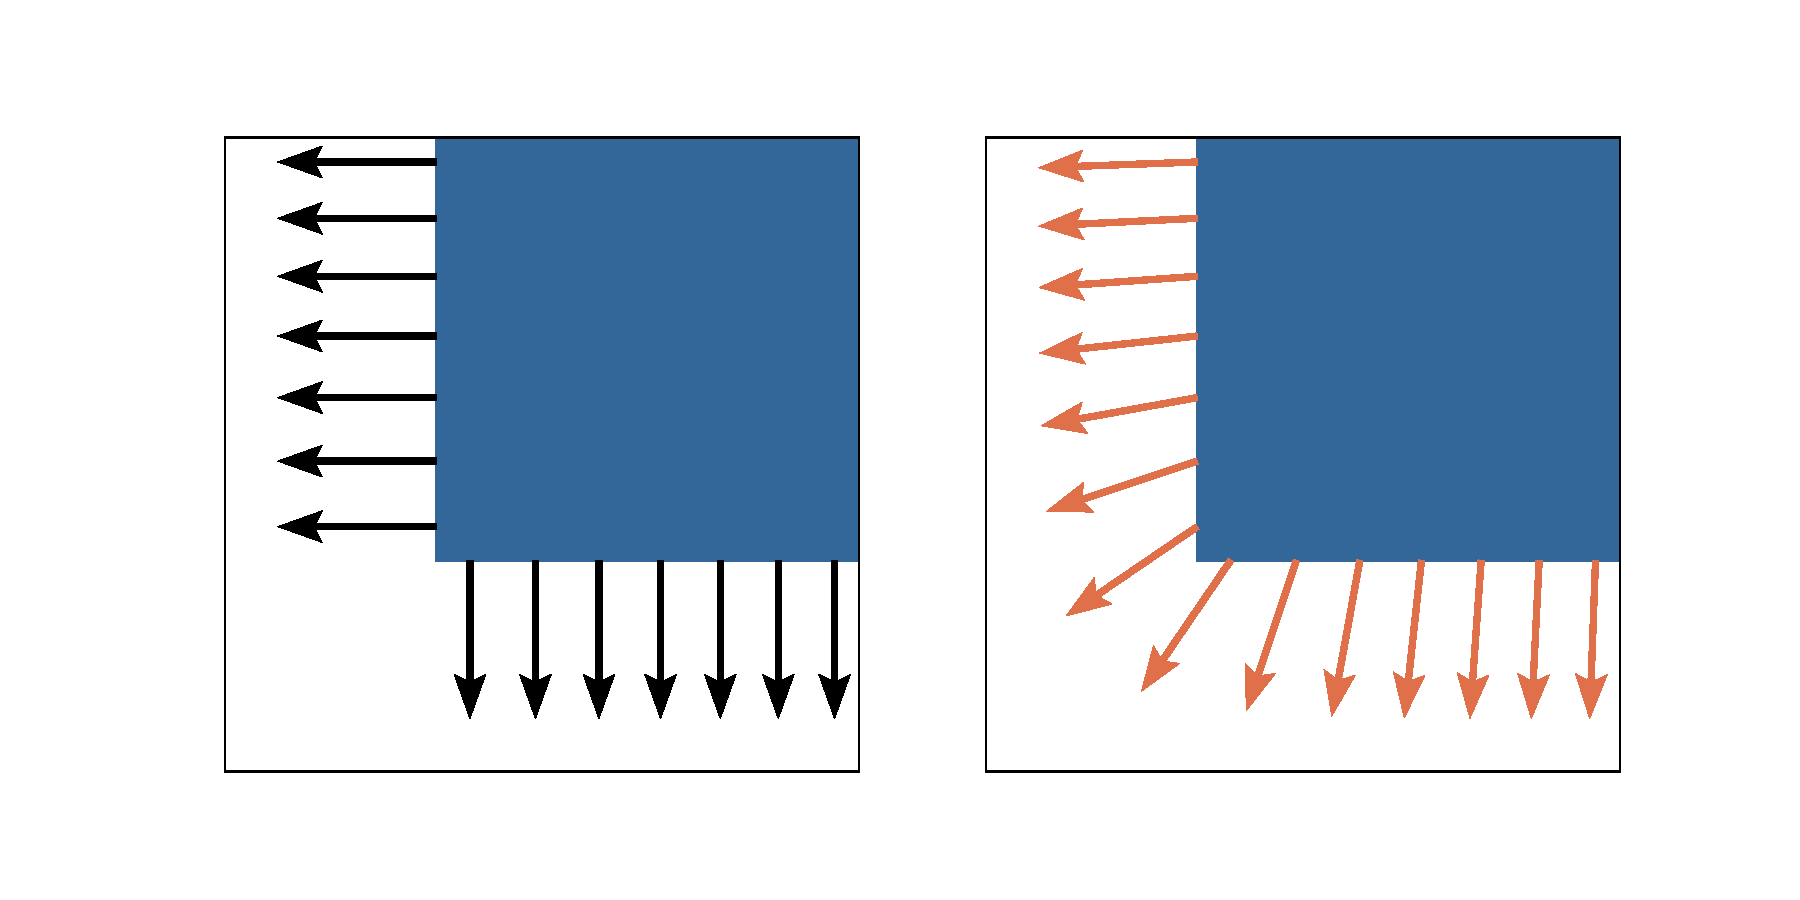
\includegraphics[width=.8\linewidth]{figures/dcol_normals_v2.pdf}

        \definecolor{CUST}{HTML}{E0704A}
        \begin{tikzpicture}
            % \draw[black, thick] (0,0.5) rectangle (6, 1);

            \draw[black, line width=2pt] (-3.7, 1.77) -- (-3.0, 1.77);
            \node[anchor=west] at (-2.8, 1.8) {$\kappa=0$};

            \draw[CUST, line width=2pt] (1.3, 1.77) -- (2.0, 1.77);
            \node[anchor=west] at (2.2, 1.8) {$\kappa=0.01$};
        \end{tikzpicture}
        \caption{Contact normal vectors from an optimization-based differentiable collision detection routine with and without relaxed differentiation. With no relaxation ($\kappa=0$), the direction of the contact normal switches immediately as the closest point moves from one face to another. When relaxed gradients are used ($\kappa=0.01$), the contact normal smoothly transitions between the faces.}
        \label{qpax:fig:dcol}
    \end{figure}
Collision detection between convex shapes can be formulated as a convex optimization problem, both in terms of the closest point between shapes \cite{gilbert1988}, and in terms of the minimum scale factor \cite{tracy2023b}. For the former, we introduce two points in a world frame $p_i \in \R{3}$, and two polytopes described with $A_i p_i \leq b_i$. By constraining each point to be within a polytope, a QP is used to solve for the closest point between these two shapes,
\begin{mini}
    {p_1, p_2}{ \|p_1 - p_2\|_2^2}{\label{qpax:gjk}}{}
    \addConstraint{A_1 p_1}{\leq b_1}%{k = 1,\ldots,N-1}
    \addConstraint{A_2 p_2}{\leq b_2.}%{k = 1,\ldots,N-1}
\end{mini}
Using a differentiable QP solver, the gradient of the objective value with respect to the positions of the polytopes results in the contact normal vectors. 

In this example, we examine collision detection between two squares and the behavior of these contact normals in the presence of sharp corners. As shown in Fig. \ref{qpax:fig:dcol}, the contact normals are evaluated at a strict $\kappa=0$ and a relaxed $\kappa=0.01$. In the case of $\kappa=0$, the contact normals are (correctly) exactly normal to the surface, and as soon as the closest point shifts from one face to the other, the contact normals immediately rotate $90^\circ$. While this is expected behavior, this discontinuity in the gradient can prove troublesome for simulation and control algorithms that rely on these contact normals not changing too quickly. Alternatively, with a relaxed $\kappa=0.01$, the contact normal smoothly rotates the 90 degrees as the face of the closest point changes. This is a result of the logarithmic barrier smoothing out the sharp corner, and allows for continuous and smooth gradients even in the presence of the discontinuity. 
% The efficacy of this approach for collision-free motion planning is demonstrated in \cite{tracy2023b}, where collision constraints are represented with differentiable optimization problems. 
\section{Conclusions}
In this paper, we outline shortcomings with existing differentiable optimization tools, namely the nonsmoothness of the gradients near inequality constraints and the inability to handle infeasible problems, and propose solutions to both of these problems. By relaxing the solution to an optimization problem from tight tolerances to an intentionally relaxed logarithmic barrier, unique and smooth gradients can be computed even from sharp edges in the feasible set. This relaxation is straightforward and leverages existing routines within existing primal-dual interior-point solvers. We also introduce an always-feasible quadratic program where hard constraints are converted into $\ell_1$-penalties, and devise a customized algorithm for solving problems of this form with limited added computational overhead. With both of these innovations, consistent and reliable smooth gradients are demonstrated in common robotic tasks where smoothness is a priority. Our fully differentiable and parallelizable solver written in JAX is available at \url{www.github.com/kevin-tracy/qpax}.
% \graphicspath{{cpeg1/}}


\chapter{Atmospheric Entry Guidance}
\label{sec:cpeg1}

As scientific and crewed payloads have more demanding goals, precise atmospheric entry guidance is playing an increasing role in mission success. State-of-the-art entry guidance algorithms are structured in a predictor-corrector framework, where a simulation is used to predict a trajectory, and corrections are then made to the control inputs.  These guidance methods are simple and effective, but current algorithms assume low lift-to-drag entry vehicles, are limited to only bank-angle control, and have a limited ability to guarantee the safety of the vehicle. We propose a new predictor-corrector entry guidance method that formulates the correction step as a convex optimization problem. This allows for more flexibility in specifying the vehicle's dynamics and control inputs, and the ability to explicitly handle safety constraints such as heating, pressure, and acceleration limits. We test the new algorithm in Mars entry scenarios similar to the Mars Science Laboratory with both bank-angle control and bank-angle plus angle-of-attack control, demonstrating both its performance and ability to generalize to future vehicle capabilities.

The contents of this chapter have been previously published at IEEE Aerospace Conference 2021 in \citet{tracy2022c}

%%%%%%%%%%%%%%%%%%%%%%%%%%%%%%%%%%%%%%
\section{Introduction}
%%%%%%%%%%%%%%%%%%%%%%%%%%%%%%%%%%%%%%
In 1971 the Soviet Union's Mars-2 spacecraft made history by entering the Martian atmosphere before impacting the surface.  Nine days later, an identical Mars-3 spacecraft performed the first soft-landing on the Martian surface, ushering in a new era in planetary exploration. NASA followed with successful Mars landings in 1976 with Viking 1 and 2 and has since then landed and operated multiple robotic systems on the Martian surface \cite{li2014}. 

Entry vehicle architectures can be divided into three broad categories \cite{li2014}: 1) Ballistic entry is an uncontrolled descent with drag as the only force, 2) unguided ballistic-lifting entry has an uncontrolled non-zero lift force, and 3) guided ballistic-lifting entry has some control over the vehicle's lift vector. Controlled entry guidance allows for the prioritization of landing locations with scientific merit instead of just those that minimize risk to the vehicle.

The Mars Science Laboratory (MSL) carrying the Curiosity rover touched down in 2012 as the first Mars entry vehicle with guided ballistic-lifting entry.  MSL had control over the vehicle bank angle during entry, enabling control of the direction of the lift vector within the lifting plane. While MSL dramatically reduced the size of the landing ellipse from over 100 km to 10 km, its guidance is still too coarse for pinpoint landings. By developing more performant entry guidance capabilities, entry vehicles could effectively place robotic or crewed landers in desirable science collection areas, including high altitude sites. 

% \section{Previous Work}
Much of the work on guidance for low lift-to-drag entry vehicles originated with the Apollo terminal guidance methods. These algorithms, as described in \cite{graves1972}, rely on control of the bank angle with simple switching manuevers to control the cross-range and down-range errors. Slightly modified versions have been developed for use with more recent Mars entry vehicles, such as in \cite{mendeck2014}.  Current research investigates the use of predictor-corrector algorithms \cite{brunner2012} to improve the landing accuracy. A popular predictor-corrector formulation that exhibits bank-angle switching behavior is the Fully Numerical Predictor-corrector Entry Guidance (FNPEG) algorithm \cite{lu2008}. In the baseline FNPEG algorithm, Newton's method is used to solve for a static bank-angle that satisfies a terminal downrange distance constraint, and the sign of the bank-angle is modulated to control crossrange errors \cite{lu2014}. Here, the prediction phase is used to generate gradients for the terminal constraint, and corrections are applied to the open-loop commanded bank-angle in an effort to satisfy these terminal constraints. This framework is simple and effective but requires significant added complexity for incorporation of safety constraints or changes to the vehicle control inputs.

Trajectory optimization for offline planning of entry vehicle trajectories has been explored in \cite{wang2016} and \cite{wang2018a}, where the nonconvex optimal control problem was solved by linearizing the nonlinear dynamics and constraints, solving a conic optimization problem with a trust region, and repeating until convergence. This successive-convexification method was used instead of standard NonLinear Programming (NLP) solvers, like SNOPT \cite{gill2005} or IPOPT \cite{wachter2006}, because it is able to directly handle second-order cone constraints instead of relying on local linear approximations. Optimal trajectories computed offline were then paired with an optimization-based tracking controller, as described in \cite{wang2016} and \cite{wang2018a}. While these formulations are able to stabilize a trajectory, there are no guarantees that safety constraints can be satisfied online. Also, the computational complexity of the trajectory-optimization formulation makes these methods intractable for real-time control onboard an entry vehicle.

The Convex Predictor-corrector Entry Guidance (CPEG) algorithm proposed in this paper combines ideas from trajectory optimization with the predictor-corrector guidance framework by solving a constrained optimization problem during the correction step.  First, the dynamics of the entry vehicle with the current control plan are simulated to a target altitude for a predicted trajectory. Next, the vehicle dynamics are linearized about the predicted trajectory and a convex trajectory optimization problem is solved that minimizes landing error. By solving for a correction using convex optimization, CPEG is able to reason about the full state and control history to inform the correction instead of just the final state.  This also allows for the vehicle's safety constraints, such as heating, pressure, and acceleration, to be explicitly included in the correction computation. Our specific contributions in this paper are:
\begin{enumerate}
    \item A general quasi-linear formulation of entry vehicle dynamics that is well-suited to numerical optimization.
    \vspace{8pt}
    \item A predictor-corrector entry guidance algorithm with a highly generalizable correction step utilizing convex optimization.
    \vspace{8pt}
    \item Customized trust regions and objective functions for entry vehicles with multiple control modalities. 
\end{enumerate}

The paper proceeds as follows: In Section \ref{sec:cpeg1:dynamics}, the classic Vinh entry vehicle dynamics are compared with a more modern Cartesian approach. In Section \ref{sec:cpeg1:trajopt}, the details of the full nonconvex trajectory optimization problem are discussed. In Section \ref{sec:cpeg1:cpeg}, the CPEG algorithm is derived. In Section \ref{sec:cpeg1:experiments}, CPEG is validated on entry vehicles with bank-angle control, as well as bank-angle and angle-of-attack control. Finally, Section \ref{sec:cpeg1:conclusion} outlines our conclusions and potential future research directions.


\section{Entry Vehicle Dynamics}
\label{sec:cpeg1:dynamics}

Despite much of the recent powered-descent guidance literature using Cartesian state representations, entry vehicles are still most often represented in spherical coordinates. In this section, the traditional entry vehicle dynamics denoted below as the ``Vinh'' model will be discussed, as well as an alternative Cartesian formulation. 

\subsection{The Vinh Model}
The classic Vinh model, presented in 1976 in \cite{busemann1976} and again a few years Later in Vinh's textbook \cite{vinh1980}, has been the standard method for simulating entry vehicles for the past 45 years. Parameterizing the entry vehicle in spherical coordinates, the state in the Vinh model contains familiar terms like latitude, longitude, and flight-path angle. Despite being highly nonlinear and prone to scaling issues, it is the most common dynamics model in the literature \cite{busemann1976,vinh1980,vinh2000,wang2018,wang2019a,lu2014,gallais2007}.

The dynamics in the Vinh model are calculated with the angle-of-attack, $\alpha$, bank-angle, $\sigma$, flight-path angle, $\gamma$, longitude, $\theta$, latitude, $\phi$, and heading angle, $\psi$. The resulting equations of motion over a planet that's rotating with a constant angular velocity $\Omega$ are,
\begin{align}
\dot{r}&=V \sin \gamma ,\label{eq:vin1}\\
\dot{\theta}&=V \cos \gamma \sin \psi /(r \cos \phi) ,\\
\dot{\phi}&=V \cos \gamma \cos \psi / r ,\\
\dot{V}&=-D-\sin \gamma / r^{2} +\Omega^{2} r \cos \phi\sin \gamma \cos \phi   -\Omega^{2} r \cos \phi \cos \gamma \sin \phi \cos \psi  ,\\
\dot{\gamma}&=L \cos \sigma / V+\left(V^{2}-1 / r\right) \cos \gamma /(V r) +2 \Omega \cos \phi \sin \psi +\Omega^{2} r \cos \phi\cos \gamma \cos \phi / V   
 \\ & \quad \quad + \Omega^{2} r \cos \phi\sin \gamma \sin \phi \cos \psi / V , \\
\dot{\psi}&=L \sin \sigma /(V \cos \gamma)+V \cos \gamma \sin \psi \tan \phi / r 
 -2 \Omega(\tan \gamma \cos \psi \cos \phi-\sin \phi) \\ 
  & \quad \quad +\Omega^{2} r \sin \phi \cos \phi \sin \psi /(V \cos \gamma) , \label{eq:vin6}
\end{align}
where $r$ is the normalized radial distance from the center of the planet, $V$ is the normalized planet-relative velocity, and L and D are the magnitudes of the lift and drag accelerations. 

This model is highly nonlinear in both the state and the control, even when the planetary motion is ignored. While the planet's angular velocity is assumed to be constant, its inclusion in the dynamics still contributes significant nonlinearities. Because of this, much of the literature ignores the planet's angular velocity \cite{wang2016}. There are also scaling issues present if these equations are naively implemented. Since $r$ and $V$ are not angles, they are usually of a much larger magnitude than the rest of the state. This can lead to poor accuracy in variable time-step integrators, as well as ill-conditioning in numerical trajectory optimization.

\subsection{Cartesian Entry Dynamics}
We have found that entry vehicle dynamics are both simpler to derive and numerically better-conditioned when represented in standard Cartesian coordinates instead of the spherical coordinates used in the Vinh formulation. This state representation is popular with the powered-descent guidance community, albeit without any aerodynamic forces in the dynamics \cite{blackmore2012, acikmese2007, acikmese2013}.

We assume a planet-fixed frame $P$ is aligned with an inertial frame $N$ along the $z$ axis. The planet spins with angular velocity $\omega \in {\mathbb{R}}^3$ in the positive $z$ direction, making the velocity of the entry vehicle the following:
\begin{align}
{}^P v  &= {}^N v  -    \omega  \times r, \label{eq:pv}
\end{align}
where $^Nv \in {\mathbb{R}}^3$ is the inertial velocity, $^Pv \in {\mathbb{R}}^3$ is the planet relative velocity, and $r \in {\mathbb{R}}^3$ is the position of the entry vehicle in the planet frame. This expression can be differentiated once more to provide the relationship between the inertial and planet-relative accelerations:
\begin{align}
{}^P a &=   {}^{N} a -       2( \omega \times {}^P v )                          -   \omega  \times (\omega \times r) .\label{eq:Pa}
\end{align}
The state of the entry vehicle can be parameterized with the planet-relative position vector $r$, and planet relative velocity ${}^P v$ denoted as just $v$, both expressed in the coordinates of the planet frame. The Cartesian dynamics can now be written in state space as,
\begin{align}
    {\begin{bmatrix} v \\ a \end{bmatrix}} &= \begin{bmatrix} 0 & I \\ -[\omega \times]^2 & -2[\omega \times] \end{bmatrix}\begin{bmatrix}r \\v  \end{bmatrix} + \begin{bmatrix} 0 \\  a_{g} + a_{D} + a_{L} \end{bmatrix},\label{eq:dynamics}
\end{align}
where $[\omega \times]$ is the skew-symmetric cross product matrix,
\begin{align}
    [\omega \times ] &= \begin{bmatrix} 0 &-\omega_3 &\omega_2 \\ 
                                     \omega_3 &0 & -\omega_1 \\ 
                                     -\omega_2 & \omega_1 & 0 \end{bmatrix}.
\end{align}
One of the main benefits of the dynamics in equation \eqref{eq:dynamics} is the linear kinematics. This means that linear approximations of the relationship between position and velocity are exact, and the only nonlinearities present are in the accelerations. The gravitational acceleration in the direction of the planet's center is expressed assuming simple spherical gravity:
\begin{align}
    a_g &= -\frac{\mu}{\|r\|^3}r,
\end{align}
 where $\mu \in \mathbb{R}$ is the standard gravitational constant for the given planet. The acceleration caused by the drag force is in the direction opposing velocity, and is calculated as,
\begin{align}
    a_D &= - \frac{1}{2m}\rho A C_d \|v\| v,
\end{align}
where $m \in \mathbb{R}$ is the mass of the entry vehicle, $\rho \in \mathbb{R}$ is the atmospheric density, $A \in \mathbb{R}$ is the aerodynamic reference area, and $C_d \in \mathbb{R}$ is the coefficient of drag.  In this work, the atmospheric density $\rho \in \mathbb{R}$ will be represented by a piecewise exponential function \cite{gallais2007}.

\begin{figure}[t]
    \centering
    \includegraphics[width = 2in]{burn.pdf}
    \caption{The $E$ frame is fixed to the entry vehicle, with $\hat{e}_1$ in the direction of the specific angular momentum vector, and $\hat{e}_2 = \hat{v} \times \hat{e}_1$. When defined in this frame, the lift vector can be expressed using only $\hat{e}_1$ and $\hat{e}_2$.}
    \label{fig:eframe}
\end{figure}

For the description of the lift acceleration, a reference frame is defined that describes a plane about the entry vehicle that is orthogonal to the velocity vector.  This two-dimensional frame, referred to as the $E$ frame and depicted in Fig. \ref{fig:eframe}, has two basis vectors described by the following:
\begin{align}
    \hat{e}_1 &=  \frac{r \times v}{\|r \times v\|}, \\ 
    \hat{e}_2 &= \frac{v \times \hat{e}_1}{\| v \times \hat{e}_1 \|} .
\end{align}
The magnitude of the lift vector is calculated as,
\begin{align}
    \|L\| &= \frac{1}{2m} C_L \rho(r) A \|v\|^2,
\end{align}
where $C_L \in \mathbb{R}$ is the coefficient of lift. In the case where the entry vehicle only has control over the bank-angle, the resulting lift acceleration can be described by the magnitude of the lift and the bank-angle:
\begin{align}
    a_L &= \|L\|(\sin(\sigma)\hat{e}_1 + \cos(\sigma)\hat{e}_2). \label{eq:bao}
\end{align}
 In the case where the entry vehicle can control both the angle-of-attack as well as the bank-angle, the lift vector can be written as,
\begin{align}
    a_L &= \|L\|(\ell_1\hat{e}_1 + \ell_2\hat{e}_2), \label{eq:fl}
\end{align}
subject to the constraint $||\ell_1^2 + \ell_2^2|| \leq 1$.
Here the lift acceleration is a linear function of the control inputs, which is a key feature when this model is linearized in an optimization problem. Both the Vinh model and the Cartesian model are nonlinear, but the Cartesian model behaves significantly better under linearization, making it a far better candidate for trajectory optimization.


\subsection{State and Control Definitions}
In the case where only the bank-angle is controlled, the state is augmented with the bank-angle, and the sole control input is the derivative of this bank-angle with respect to time. This allows for cost functions that specify desired behavior for the derivative of the bank-angle, with the state and control as the following:
\begin{align}
x &= \begin{bmatrix} r^T & v^T & \sigma \end{bmatrix} ,\\ 
u &= \dot{\sigma}.
\end{align}
These dynamics are now in control-affine form with linear kinematics.  For the case with actuation of both the bank angle and angle-of-attack, the state and control are the following:
\begin{align}
x &= \begin{bmatrix} r^T & v^T \end{bmatrix}^T ,\\ 
u &= \begin{bmatrix} \ell_1 & \ell_2 \end{bmatrix}^T,
\end{align}
where $\ell_1$ and $\ell_2$ were defined in \eqref{eq:fl}. 
\section{Trajectory Optimization}
\label{sec:cpeg1:trajopt}
Feedback control laws for entry vehicles suffer in performance due to the severe underactuation of the vehicle. This is, in part, due to the fact that an entry vehicle has very limited ability to speed up or slow down in the along-track direction. To deal with this, it makes more sense to solve the guidance problem with a holistic planning approach, one that can reason about this limited control authority and plan for it. Therefore, we pose this problem as a trajectory optimization problem, where a locally optimal state trajectory and control plan can be solved for numerically.
%  \subsection{Reachable Set}
%  \todo{i kinda want to delete this section}
%  Given a bank-angle with a maximum angle-of-attack, the entry vehicle is able to control its final landing spot for the parachute deployment. To validate the dynamics model and view the possible places that the entry vehicle could deploy the parachute given this maximum allowable angle-of-attack, a set of simulations were run such that all of the possible bank-angles were sampled. The resulting plot is available in figure \ref{fig:reachable_set}, and is also known as the "landing footprint". This plot demonstrates that the entry vehicle does not have full controllabilty of the state and can't stabilize about a given trajectory, but it is able to fully articulate the spot in which the vehicle reaches an altitude of 10 km for the parachute deployment. This is critical because the objective of this control law is not to drive the state to a goal state at a goal time, but rather simply control the point in which the parachute system is deployed. 
% \begin{figure}
%     \centering
%     \includegraphics{tikz_figz/footprint.tikz}
%     \caption{Visualized reachable set for entry vehicle trajectories with only bank-angle control. Presented is a top view of 100 trajectories with varying bank-angle, each trajectory terminates at an altitude of 10 km.}
%     \label{fig:reachable_set}
% \end{figure}
 \subsection{Safety Constraints}
 Three key vehicle safety constraints --- heating, pressure, and acceleration --- are most dependent on the atmospheric density. Unfortunately, this is also the part of the environment in which there is the largest amount of uncertainty. The atmospheric density is often only known to roughly within a factor of two, with even less known about the wind conditions \cite{gallais2007}.
 
 The heating constraint has to do with the max allowable heat rate that the ablative heat shield can withstand \cite{edquist2007}. This is measured in power per square centimeter, and it is expressed as the following:
 \begin{align}
     \dot{Q} = k_q \sqrt{\rho}V^{3.15} \leq \dot{Q}_{max}. \label{eq:con_heat}
 \end{align} 
 This function is nonlinear but can be locally approximated with linear functions during the correction step.  The next safety constraint is the maximum dynamic pressure on the entry vehicle, which is expressed as the following:
 \begin{align}
     q = .5 \rho V^2 \leq q_{max}.\label{eq:con_press}
 \end{align}
 The last safety constraint is the maximum allowable normal load, which is the total aerodynamic force on the entry vehicle. This is expressed as a norm of the lift and drag forces:
 \begin{align}
     a = \sqrt{\|L\|^2 + \|D\|^2} \leq a_{max}.\label{eq:con_load}
 \end{align}
\subsection{Full Nonconvex Formulation}

In order to formulate a convex correction problem, we first consider the full nonlinear non-convex problem. First, the dynamics described in equation \eqref{eq:dynamics} are discretized with an explicit integrator like the classic fourth-order Runge-Kutta method \cite{montenbruck2002}, giving a discrete-time dynamics model of the form,
\begin{align} \label{eq: discrete-dynamics}
    x_{k+1} &= f(x_k,u_k,\Delta t_k).
\end{align}
No assumptions have been made about the control configuration in this dynamics model: it can account for either bank-angle-only or bank-angle plus angle-of-attack control. The full nonlinear trajectory optimization problem has the form,
% \begin{mini!} \label{nlp}
% {x,u,\Delta t}{x}{}{}
% %   {x,u,\Delta t}{\ell_N(x_N, u_N)+ \sum_{k=1}^{N-1}\ell_k(x_k, u_k) }{}{}
% %   \addConstraint{x_{k+1}}{= f(x_k,u_k,\Delta t_k),}{\forall k}
% %   \addConstraint{g_k(x_k, u_k)}{\leq 0,}{\forall k}
% %   \addConstraint{\Delta t_{min} \leq \Delta t_k }{\leq \Delta t_{max} }{\forall k}
% %   \addConstraint{x_N}{=x_{goal}}{},
% \end{mini!}
\begin{mini}<b>
  {x,u,\Delta t}{\ell_N(x_N, u_N)+ \sum _{k=1}^{N-1}\ell_k(x_k, u_k) }{}{}
  \addConstraint{x_{k+1}}{= f(x_k,u_k,\Delta t_k)}{\forall k} \labelOP{nlp}%\tag{test}
  \addConstraint{g_k(x_k, u_k)}{\leq 0}{\forall k} 
  \addConstraint{\Delta t_{min} }{\leq \Delta t_k \leq \Delta t_{max} }{\forall k}
  \addConstraint{x_N}{=x_{goal}}{},
 \end{mini}
 where safety constraints \eqref{eq:con_heat}---\eqref{eq:con_load} are included in the inequality constraint function $g_k(x_k, u_k)$. Note that this is a free-final-time problem in which the $\Delta t_k$ are decision variables in addition to the states and controls. This is necessary due to the inability of the entry vehicle to reach its goal state at an arbitrarily specified time. Problem \eqref{nlp} is nonconvex due to both the nonlinear dynamics, as well as the variable time between knot points. It is worth noting that, even with linear continuous-time dynamics, the discrete-time dynamics constraints \eqref{eq: discrete-dynamics} become nonlinear when the time step is made to be a decision variable.
 %This time step variable is bounded between two positive values to ensure the dynamics progress forward, and the dynamics don't take larger steps than is appropriate given the accuracy of the integrator. 
 
 Trajectory optimization problems like \eqref{nlp} can be solved with a variety of methods. One standard approach is to use an off-the-shelf NLP solver like IPOPT \cite{wachter2006} or SNOPT \cite{gill2005}. Alternatively, more specialized trajectory optimizers like ALTRO can be used \cite{howell2019,jackson2021}.  While computationally tractable using one of the described methods, the nonconvexity of the problem means there are no available guarantees for the quality of the solution or convergence of the solver. As a result, running nonconvex trajectory optimization onboard safety-critical aerospace systems is unpopular, explaining the prevalence of simpler heritage methods for entry guidance. 

 \section{Convex Predictor-corrector}
\label{sec:cpeg1:cpeg}
CPEG combines ideas from numerical trajectory optimization with the classic predictor-corrector guidance framework: It uses a prediction step, in which the vehicle dynamics are simulated until a target altitude is reached, combined with a corrector step that is based on solving a local convex approximation of a nonlinear trajectory optimization problem to steer the vehicle to the desired target. These steps are then repeated until convergence is achieved. This section provides a detailed derivation of the CPEG algorithm.

\subsection{Prediction and Dynamics Linearization}

In the first stage of CPEG, the dynamics of the entry vehicle are simulated with a standard Runge-Kutta method using the current nominal control trajectory, $\bar{U}$, until a target altitude is reached. We denote this predicted trajectory by $\bar{X}$. After the prediction step, the discrete-time nonlinear dynamics are approximated using a first-order Taylor series,
\begin{align}
    \bar{x}_{k+1} + \delta x_{k+1} \approx f(\bar{x}_k,\bar{u}_k) + A_k \delta x_k + B_k \delta u_k,
\end{align}
where $A_k$ and $B_k$ are the following Jacobians,
\begin{align}
    A_k &= \frac{\partial f(x_k,u_k,\Delta t_k)}{\partial x_k} \bigg\rvert _{\bar{x}_k,\bar{u}_k}, \label{jacob1}\\
    B_k &= \frac{\partial f(x_k,u_k,\Delta t_k)}{\partial u_k}\bigg\rvert _{\bar{x}_k,\bar{u}_k}. \label{jacob2}
\end{align}
Subtracting the dynamics of the reference trajectory from both sides, the local linear dynamics of trajectory corrections can be written as:
\begin{align}
    \delta x_{k+1} = A_k \delta x_k + B_k \delta u_k.\label{eq:linmod}
\end{align}
A crucial distinction between CPEG and sequential convexification methods \cite{wang2016,malyuta2021,mao2019}, is that trajectory iterates are always dynamically feasible, thanks to the prediction step. This eliminates the possibility of inconsistent linearizations of the dynamics constraints \cite{nocedal2006}, in which no feasible correction trajectory exists. Specifically, there is always a trivial solution to \eqref{eq:linmod} of all zeros for $\delta x$ and $\delta u$.

\subsection{Cost Function}
The cost function used in CPEG is comprised of a term that penalizes the miss distance from the target and a term that penalizes specified control behaviors. For the penalty on miss distance, putting a naive quadratic cost on the error between the final position and the desired position is inappropriate since it also penalizes altitude errors. Instead, only the position error projected onto the landing plane is penalized, effectively ignoring altitude error. Since the altitude target is implicitly satisfied during the prediction step, this allows for the correction to only apply changes to the control plan that minimize the projected miss distance. The cost function for this projected miss distance is the following:
\begin{align}
\ell_{miss}(\delta X,\delta U) &= \|W( r_N + \delta r_N - r_{goal})\|_2^2 ,\label{eq:miss}
\end{align}
where $r_N \in {\mathbb{R}}^3$ is the  final position in the reference trajectory, $\delta r_N \in {\mathbb{R}}^3$ is the correction computed for this position, and $r_{goal} \in {\mathbb{R}}^3$ is the desired final position for parachute deployment. To project this error onto the landing plane, we define following projection matrix, 
\begin{align}
W &= I - pp^T,
\end{align}
where $p$ is the unit vector normal to the planetary surface at the target position:
\begin{align}
p &= \frac{r_{goal}}{\|r_{goal}\|}.
\end{align}
The second part of the cost function seeks to shape the control behavior. In the case of bank-angle control, we consider two different control cost functions that produce qualitatively different behavior:
\begin{align}
    \ell_{\sigma,L1}(\delta U) &= \lambda \|\dot{\sigma_k}\|_1, \label{eq:bankl1}
\end{align}
and
\begin{align}
    \ell_{\sigma,quad}(\delta U) &= \lambda \dot{\sigma_k}^2, \label{eq:bankl2}
\end{align}
where $\lambda$ is a scalar tuning parameter. The first cost function \eqref{eq:bankl1} penalizes the L1 norm of the derivative of the bank-angle, resulting in bank-angle trajectories with a minimum number of discrete switches. The second cost function \eqref{eq:bankl2} penalizes the square of the bank-angle derivative, resulting in smooth bank-angle trajectories. For the bank-angle plus angle-of-attack case, as described in \eqref{eq:fl}, we apply a simple quadratic cost to the norm of the controlled lift vector, effectively penalizing high angles of attack:
\begin{align}
    \ell_{\sigma \alpha}(\delta U) &= \lambda \|u_k\|_2^2. \label{eq:baoa_cost}
\end{align}
\subsection{Constraints}
Of the three nonlinear safety constraints, two can be linearized, and the third can be converted to a conservative convex relaxation. For the heating and dynamic pressure constraints \eqref{eq:con_heat}--\eqref{eq:con_press}, a Taylor expansion of each is formed, approximating the constraint to first-order. From here, a linearized inequality constraint can be directly included in the convex correction problem. For these constraints, the linearized versions are:
\begin{align}
 [\nabla \dot{Q}(\bar{x}_k)]^T \delta x_k &\leq \dot{Q}_{max} - \dot{Q}(\bar{x}_k), \label{eq:lincon_heat}\\ 
  [\nabla {q}(\bar{x}_k)]^T \delta {x}_k &\leq {q}_{max} - {q}(\bar{x}_k). \label{eq:lincon_press}
\end{align}
The acceleration loading constraint \eqref{eq:con_load} is nonlinear, but a conservative convex relaxation can be derived in the form of a second-order cone constraint. First, the kinematics for the velocity can be conservatively approximated as the following:
\begin{align}
v_{k+1} &= v_k + a_k \Delta t, \\ 
a_k &= \frac{v_{k+1} - v_k}{\Delta t}, \\
a_k &=  \frac{\bar{v}_{k+1} + \delta v_{k+1} - \bar{v}_k - \delta v_k}{\Delta t}.
\end{align}
The maximum loading constraint can then be re-written as,
\begin{align}
% \|a_k\|_2 = \frac{1}{\Delta t} \|\bar{v}_{k+1} + \delta v_{k+1} - \bar{v}_k - \delta v_k\| &\leq a_{max} \\
 \|\bar{v}_{k+1} + \delta v_{k+1} - \bar{v}_k - \delta v_k\| &\leq  \Delta t \cdot a_{max}, \label{eq:lincon_accel}
\end{align}
which is in the form of a convex second-order cone, and can be directly incorporated into the correction problem.

The three  safety constraints from equations \eqref{eq:lincon_heat}, \eqref{eq:lincon_press}, and \eqref{eq:lincon_accel}, are stacked into a generic safety constraint function, 
\begin{align}
g_{safety}(\delta x_k, \delta u_k) &\leq 0 . 
\end{align}
\subsection{Trust Region}
To ensure that corrections are sufficiently small that the dynamics linearizations and constraint approximations remain accurate, a trust-region constraint is added to the convex correction problem. While standard trust-region methods apply norm constraints to $\delta  X$ and $\delta U$ \cite{nocedal2006}, insight into the entry guidance problem enables a more tailored approach. 

The quality of the linearization presented in \eqref{eq:linmod} is highly accurate for approximating the vehicle kinematics, gravity, and atmospheric drag, but is much less accurate when applied to the bank-angle in the bank-angle-only control case. Therefore, we design a trust region that restricts corrections to the bank-angle, $\delta \sigma_k$, given the known accuracy of small-angle approximations but allows large corrections to the other states. This approach also allows us to avoid the need to adapt trust regions inside the solver, enabling faster and more reliable convergence. We apply the following trust-region constraints to each corrector problem:
\begin{align}
\|\delta u_k\|_2 &\leq \delta u_{max}\\
|\delta \sigma_k | &\leq \delta \sigma_{max}
\end{align}
\subsection{Convex Corrector Problem}
For the case where the entry vehicle has control of only the bank-angle as described in \eqref{eq:bao}, the convex correction problem can be formulated as,
\begin{mini}
  {\delta X, \delta U}{\ell_{miss}(\delta X, \delta U) + \ell_{\sigma }(\delta U)}{\label{cpeg_boa}}{}
  \addConstraint{A_k \delta x_k + B_k \delta u_k}{=\delta x_{k+1}}{}
  \addConstraint{g_{safety}(\delta x_k, \delta u_k)}{\leq 0}{}
  \addConstraint{\|\delta u_k\|_2}{\leq \delta u_{max}}{}
  \addConstraint{|\delta \sigma_k |}{\leq \delta \sigma_{max},}{}
 \end{mini}
where the miss cost function is described in \eqref{eq:miss}, and the bank-angle cost function can be either \eqref{eq:bankl1} or \eqref{eq:bankl2}.

For the case where the entry vehicle has control over both bank-angle and angle-of-attack as described in \eqref{eq:fl}, the convex correction problem can be posed as:
\begin{mini}
  {\delta X, \delta U}{\ell_{miss}(\delta X, \delta U) + \ell_{\sigma \alpha}(\delta U)}{\label{cpeg_fl}}{}
  \addConstraint{A_k \delta x_k + B_k \delta u_k}{=\delta x_{k+1}}{}
  \addConstraint{g_{safety}(\delta x_k, \delta u_k)}{\leq 0}{}
  \addConstraint{\|u_k + \delta u_k\|_2}{\leq 1.}{} 
 \end{mini}
%A key difference here is that there is now a unit norm constraint on $u + \delta u$, ensuring the normalized lift control input does not exceed the maximum allowable lift.

These problems can be solved quickly and reliably by standard conic solvers such as Mosek \cite{mosekaps2014}, COSMO \cite{garstka2020}, and ECOS \cite{domahidi2013}.
%The trust region constraints ensure that the solution to this problem is within a reasonable region of linearization, allowing for the correction to be applied to the control plan with confidence.
 \subsection{CPEG Algorithm}
 The full CPEG algorithm is detailed in algorithm \ref{alg:flight}. The inputs to CPEG are the current position and the current control plan. From here, the dynamics of the entry vehicle are simulated until parachute deployment with the current control plan. This predicted trajectory is then discretized and linearized, resulting in dynamics Jacobians $A_k$ and $B_k$ (equations \eqref{jacob1}-\eqref{jacob2}). From here, the convex correction problem is posed given the control configuration and cost strategy. This convex optimization problem is solved, and the correction $\delta U$ is used to correct the control plan. The prediction-correction steps are repeated until the norm of the correction being made to the control plan is below a specified tolerance. 
  \begin{algorithm} 
	\begin{algorithmic}[1]
		\caption{CPEG Algorithm}\label{alg:flight}
		\State \textbf{input} $x_0$, U  \Comment{nominal control plan}
		\While{$\|\delta U\| > $ tolerance}
    		\State $\Bar{X}, \Bar{U} = \text{simulate}(x_0,U)$ \Comment{predict trajectory}
    		\State $A,B = \text{linearize}(\Bar{X}, \Bar{U})$ \Comment{linearize about prediction}
    		\State $\delta X,\delta U = \text{cvx}(\Bar{X}, \Bar{U}, A, B)$ \Comment{solve for correction} 
    	    \State $U \mathrel{+}= \delta U $ \Comment{correct control plan}
		\EndWhile
		\State \textbf{return} $U$ \Comment{return updated control plan}
	\end{algorithmic}
\end{algorithm}

\section{Numerical Experiments}
 \label{sec:cpeg1:experiments}
Parameters roughly matching those of the Mars Science Laboratory (MSL) \cite{mendeck2014} were used to test the CPEG algorithm. All scenarios begin at an altitude of $125$ km above the Martian surface with a Mars-relative velocity of 5.845 km/second. CPEG was implemented in the Julia programming language \cite{bezanson2017}, using the Convex.jl optimization modeling library \cite{udell2014}, and the Mosek \cite{mosekaps2014} and OSQP \cite{stellato} solvers. CPEG was validated on the following three cases:
\begin{itemize}
    \item Bank-angle control with L1 cost penalty, denoted $\sigma_{L1}$.
    \vspace{+2mm}
    \item Bank-angle control with quadratic penalty, denoted $\sigma_{2}$.
    \vspace{+2mm}
    \item Bank-angle plus angle-of-attack control, denoted $\sigma + \alpha$.
\end{itemize}
For the bank-angle cases, CPEG was arbitrarily initialized with a constant bank-angle of zero, with noise added to the bank-angle derivative. For the bank-angle plus angle-of-attack case, a similar approach was used, but noise was added to the normalized lift vector. The final converged trajectories for the three cases are shown in figures \ref{fig:allalt} and \ref{fig:allcrdr}. In all of the cases, CPEG was able to successfully guide the entry vehicle to the target point at the desired altitude.
\begin{figure}
    \centering
    \includegraphics{cpeg1/tikz/all_altdr.tikz}
    \caption{Altitude and downrange distance from the converged trajectories from CPEG on the three specified cases. The $\sigma_{L1}$ case is with bank-angle control and an L1 penalty on bank-angle derivative, $\sigma_{quad}$ is bank-angle only with a quadratic penalty on bank-angle derivative, and $\sigma + \alpha$ is control over both bank-angle and angle-of-attack. Due to the differences in control authority and cost function, all three converge on different trajectories that hit the target position at parachute deployment.}
    \label{fig:allalt}
\end{figure}
% \todo{Describe what the different cases are in all of the figure captions as well (i.e. spell out what the labels mean).}
\begin{figure}
    \centering
    \includegraphics{cpeg1/tikz/all_crdr.tikz}
    \caption{Crossrange and downrange trajectory data from the converged trajectories from CPEG on the three specified cases. The cases with only control over the bank-angle have to do a bank reversal to hit the target, whereas the case with control over bank-angle and angle-of-attack is able to leverage the full lift control to avoid the switching.}
    \label{fig:allcrdr}
\end{figure}
\subsection{Bank-Angle Control}
For the case where the entry vehicle has only bank-angle control, the convergence of CPEG can be observed in figures \ref{fig:l1alt} and \ref{fig:l1crdr} for the case with an L1 cost on the bank-angle derivative, and figures \ref{fig:l2alt} and \ref{fig:l2crdr} with a quadratic cost.  These plots show the output of the prediction step of CPEG, where the color of the predictions is blue for the first iteration of the algorithm and turns purple, then pink for later iterations.
\begin{figure}
    \centering
    \includegraphics{cpeg1/tikz/L1_altdr.tikz}
    \caption{Predicted entry vehicle trajectories for the bank-angle only L1 penalty case, as seen by the altitude and downrange data. As the iterates continue, the entry vehicle converges on a trajectory that reaches the target at the 10km altitude mark.} 
    \label{fig:l1alt}
\end{figure}
\begin{figure}
    \centering
    \includegraphics{cpeg1/tikz/L1_crdr.tikz}
    \caption{Predicted entry vehicle trajectories for the bank-angle only L1 penalty case, as seen by the crossrange and downrange data.}
    \label{fig:l1crdr}
\end{figure}
  \begin{figure}
    \centering
    \includegraphics{cpeg1/tikz/L2_altdr.tikz}
    \caption{Predicted entry vehicle trajectories for the bank-angle only quadratic penalty case, as seen by the altitude and downrange data. The}
    \label{fig:l2alt}
\end{figure}
\begin{figure}
    \centering
    \includegraphics{cpeg1/tikz/L2_crdr.tikz}
    \caption{Predicted entry vehicle trajectories for the bank-angle only quadratic penalty case, as seen by the crossrange and downrange data.}
    \label{fig:l2crdr}
\end{figure}
After convergence, the two bank-angle profiles that CPEG produced for the L1 and quadratic cost functions are shown in figure \ref{fig:banks}. The L1 cost on the derivative of the bank-angle encouraged sparsity in this derivative, resulting in a bank-angle profile that switches between constant bank-angles. For the case with a quadratic cost on the bank-angle derivative, the resulting bank-angle profile is smooth with no discrete switching behavior.
\begin{figure}
    \centering
    \includegraphics{cpeg1/tikz/banks.tikz}
    \caption{Bank-angle only control plans for both the L1 and quadratic cost cases. The L1 cost motivated a bang-bang switching style bank-angle profile. The quadratic cost resulted in a smooth and continuous bank-angle profile.}
    \label{fig:banks}
\end{figure}
\subsection{Bank-Angle and Angle-of-Attack Control}
As described by the dynamics in equation \eqref{eq:fl}, the control input for this case is the lift vector itself in the directions orthogonal to the velocity vector. This allows for manipulation of both the bank-angle and angle-of-attack and is guaranteed to be within the maximum allowable lift by the unit norm constraint in equation \eqref{cpeg_fl}. In this control case, the control input Jacobian is constant and independent of the nominal control plan, making the linearization significantly more accurate than the bank-angle-only case. As a result, the convergence of CPEG with bank-angle plus angle-of-attack control is significantly faster than with the bank-angle alone. The evolution of the predicted trajectories is shown in figures \ref{fig:flalt} and \ref{fig:flcrdr}, with the same coloring scheme as the bank-angle only section. After convergence, the control inputs were converted back into bank-angle and angle-of-attack and shown together in figure \ref{fig:flcontrols}.
\begin{figure}
    \centering
    \includegraphics{cpeg1/tikz/FL_altdr.tikz}
    \caption{Predicted entry vehicle trajectories for the bank-angle and angle-of-attack case, as seen by the altitude and downrange data.}
    \label{fig:flalt}
\end{figure}
\begin{figure}
    \centering
    \includegraphics{cpeg1/tikz/FL_crdr.tikz}
    \caption{Predicted entry vehicle trajectories for the bank-angle and angle-of-attack case, as seen by the crossrange and downrange data.}
    \label{fig:flcrdr}
\end{figure}
\begin{figure}
    \centering
    \includegraphics{cpeg1/tikz/fl_controls.tikz}
    \caption{Bank-angle and angle-of-attack profiles for the case where both angles are being controlled. CPEG was able to converge on this control plan in just three iterations.}
    \label{fig:flcontrols}
\end{figure}
\section{Conclusion}
\label{sec:cpeg1:conclusion}
This paper proposes an improved version of the classic predictor-corrector entry guidance scheme in which the correction step is formulated as a convex optimization problem. Two control strategies were tested with CPEG: bank-angle control, and bank-angle plus angle-of-attack modulation. For the bank-angle-only case, cost functions that penalized the derivative with an L1 cost and a quadratic cost were both demonstrated, resulting in dramatically different optimal bank-angle profiles. For the case with both bank-angle and angle-of-attack control, the quality of the dynamics linearization was accurate enough that CPEG was able to converge on an optimal trajectory in just a few iterations. An implementation of CPEG running all of the examples in this paper is available at \url{https://github.com/RoboticExplorationLab/EntryGuidance.jl}.
% \graphicspath{{cpeg2/}}


\chapter{Robust Entry Guidance with Atmospheric Adaptation}
\label{sec:cpeg2}

Robust atmospheric entry guidance for blunt-body entry vehicles with bank angle modulation is achieved by combining online atmospheric density estimation with an updated version of the Convex Predictor-corrector Entry Guidance (CPEG) algorithm. During atmospheric entry, a square-root Extended Kalman Filter is used to estimate a ratio between the density of the experienced atmosphere with that of an approximate model, which is spline-fit based on MarsGRAM perturbed data. The information from this filter is used to modify the approximate model used by the guidance algorithm. The proposed update to CPEG includes time as a decision variable, dramatically improving the robustness of the algorithm. CPEG predicts the trajectory at each control call with a nonlinear simulation followed by a single convex trajectory optimization problem that updates the commanded bank angle derivative. The robustness and performance of this estimator and controller guidance architecture are demonstrated on a wide range of realistic Martian atmospheres and is able to achieve state-of-the-art accuracy with respect to altitude-triggered parachute deployment.

The contents of this chapter have been previously published at IEEE Aerospace Conference 2021 in \citet{tracy2023}
% \graphicspath{{wigglesat/}}


\chapter{Ultra-Fine Pointing for Nanosatellite Telescopes With Actuated Booms}
\label{sec:wigglesat}

The smallsat revolution has impacted the architecture of most modern satellites with the notable exception of fine-pointing space telescopes. Conventional attitude control hardware scales poorly as the spacecraft gets smaller, resulting in significant mass and performance penalties for nanosatellites with strict pointing requirements. This paper presents a novel attitude actuation and planning strategy that utilizes actuated booms with tip masses and magnetorquers for three-axis pointing and momentum desaturation. The speed of the booms is an appropriate match for the slowly varying environmental disturbance torques encountered in low-Earth orbit. As a result, these booms do not create the high-frequency jitter that reaction wheels do, lessening the need for complex second-stage correction hardware in the payload. An optimization-based motion planner is able to reason about the orbital ephemeris to ensure the booms never exceed their actuation limits, and a Linear Quadratic Gaussian controller is able to maintain fine-pointing during times of payload operation.

The contents of this chapter have been previously published at IEEE Aerospace Conference 2021 in \citet{tracy2022a}.

\section{Introduction}
Space telescopes have been able to explore the universe in ways that terrestrial telescopes cannot through the atmosphere. Current monolithic systems like the Hubble Space Telescope use onboard reaction wheels or Control Moment Gyroscopes (CMGs) to control pointing \cite{beals1988}. These actuators spin weighted rotors onboard the spacecraft to store angular momentum and maintain pointing in the presence of disturbance torques.  Unfortunately, the fractional mass of traditional attitude-control hardware grows dramatically as the spacecraft gets smaller. For larger satellites, the actuators take up only a few percent of the total spacecraft mass but, as the spacecraft gets smaller, it can consume 30\% or more of the total mass \cite{douglas2021}.% and CMG are generally impractical on CubeSat scales \cite{votel_comparison_2012}.

One issue with modern attitude control hardware on nanosatellites comes from the vibrations present in reaction wheel and CMG operation. These actuators have to spin at high angular velocities to store the required onboard angular momentum, and small defects or imbalances in the rotors cause high-frequency jitter. These vibrations can resonate with structural modes in the satellite and can corrupt payload pointing performance. To deal with image-corrupting jitter, nanosatellite payloads employ second-stage corrections to enable finer pointing performance for the payload than the body of the spacecraft. Common methods for accomplishing this are fast-steering optical mirrors, image plane shifting with lead zirconate titanate (PZT) actuators, and image stabilization \cite{serra2021,pong,ponga,allan2018}.  
These highly complex electromechanical systems are expensive and must be tailored to a specific payload, increasing costs and payload size, weight, and power (SWaP).
\begin{figure}[t!]
    \centering
    \includegraphics[width=12cm]{Figures/view1.png}
    \caption{Proposed architecture for a 6U CubeSat space telescope. Each boom has a single degree-of-freedom in linearly independent axes, enabling three-axis attitude control. Magnetorquers are used to desaturate the angular momentum of the booms and keep them within their operating limits.}
    \label{fig:meshcat_shot}
\end{figure}

In this paper, a novel actuation strategy for fine-pointing nanosatellites is explored by abandoning high-frequency rotor-based actuators in favor of low-frequency deployable booms, as shown in Figure \ref{fig:meshcat_shot}. By taking advantage of the squared relationship between boom length and the inertia of the boom, tip-mounted masses provide the control authority required for attitude control without having to accelerate or decelerate the booms too aggressively. A nanosatellite would deploy three booms about linearly independent axes and rotate them \textit{slowly} to reject the \textit{slowly} varying disturbance torques. By better matching the actuators' speed to the frequency content of the disturbances, these booms are able to eliminate jitter and enable high-accuracy body pointing of the nanosatellite. By improving body pointing, payloads are no longer restricted to those that can accommodate second-stage correction, and existing payloads can be simplified. 

For nanosatellites in low-Earth orbit, disturbance torques come in the form of drag, solar radiation pressure, magnetic, and gravity-gradient torques. All of these disturbances vary slowly throughout an orbit and can be predicted or estimated with high accuracy.  With knowledge of the incoming disturbance torques, the nanosatellite can formulate a motion plan that accounts for disturbances and keeps the deployable booms from hitting their hard stops by using the onboard magnetorquers to offload angular momentum through interactions with the Earth's magnetic field \cite{gatherer2019,markley2014}. Since nominal operations have the nanosatellites inertially pointing during payload operations, linearized attitude dynamics are sufficiently accurate for planning purposes. This allows for a convex formulation of the motion-planning problem, guaranteeing a globally optimal solution in polynomial time \cite{boyd2004}. 

Our primary contributions in this paper include:
%\vspace{-1em}
\begin{enumerate}
\item The introduction of a novel attitude-actuation strategy for fine-pointing nanosatellites.
\vspace{+2mm}
%\item A frequency analysis of the environmental disturbance torques present on a satellite in low-Earth orbit. \todo{this is from our other paper technically}
\vspace{+2mm}
\item The application of convex optimization to motion planning for nanosatellites with actuated booms.
\vspace{+2mm}
\item An estimator and controller architecture for handling boom control during payload operations.
\end{enumerate}
%\vspace{-1em}

In the remainder of this paper, we first provide details on the simulation environment used for this research in Section~\ref{sec:wigglesat:simenv}. Next, the deployable-boom actuation strategy is discussed in Section \ref{sec:wigglesat:actuation}, and a convex motion planner is developed in Section \ref{sec:wigglesat:planner} to reason about the actuator's constraints.  A lower-level estimation and control architecture is then detailed in Section \ref{sec:wigglesat:control}. Finally, numerical experiments are presented in Section \ref{sec:wigglesat:experiments} to validate the proposed ideas, and results are summarized in Section \ref{sec:wigglesat:conclusion}.

\section{Spacecraft Dynamics Model}
\label{sec:wigglesat:simenv}
This section describes the model used to analyze and simulate the dynamics of a nanosatellite space telescope in low-Earth orbit. Since the spacecraft has no propulsion onboard, the orbital and attitude dynamics are decoupled and can be modeled separately. The open-source Julia package \textit{SatelliteDynamics.jl} is used for orbital simulation, taking into account high order gravity, atmospheric drag, solar radiation pressure, and third-body accelerations. For the attitude dynamics, a rigid-body simulation is used that includes the disturbance torques present in low-Earth orbit. 

We denote the Earth-Centered Inertial frame (ECI) as $\mathbb{E}$, and the spacecraft body frame as $\mathbb{B}$. Relating these two frames is ${}^{\mathbb{B}} Q {}^{\mathbb{E}}$, the rotation matrix that takes vectors expressed in $\mathbb{E}$ and resolves them in frame $\mathbb{B}$.
\subsubsection{Gravity-Gradient Torque}
Gravity varies inversely with the square of the distance from the central body. Because of this, parts of the spacecraft that are farther away from the center of the central body experience a smaller gravitational force than the parts that are closer. The resulting non-uniform gravitational force acting on the spacecraft causes a torque. This torque can be neatly expressed in terms of the spacecraft's attitude, orbital position, and the inertia \cite{markley2014,wertz1978}. First, the normalized position vector is computed in the body frame:
\begin{align}
    \hat{m} &= \frac{{}^{\mathbb{B}} Q {}^{\mathbb{E}} r_{\mathbb{E}}}{\|r_{\mathbb{E}}\|},
\end{align}
then, the gravity-gradient torque can be calculated, 
\begin{align}
    \tau_{gg} &= \frac{3 \mu}{\|r\|^3}(\hat{m} \times J\hat{m}),
\end{align}
where $\mu$ is the standard gravitational parameter for Earth. This calculation only takes into consideration the spherical gravitational term, since the gravity gradient torque from higher-order gravity terms is of negligible magnitude.  For inertially pointing spacecraft in pure Keplerian motion, the resulting gravity gradient torque is periodic with the orbit.

\subsubsection{Atmospheric Drag Torque}
To describe the atmospheric drag torque, the relative velocity of the spacecraft with respect to the atmosphere is calculated with the following:
\begin{align}
    v_{rel} = {}^{\mathbb{B}} Q {}^{\mathbb{E}} ( v_{eci} - \omega_{Earth} \times r_{\mathbb{E}} ).
\end{align}
A normalized version of this vector will be represented as $\hat{v}_{rel} = v_{rel}/\|v_{rel}\|$.
The spacecraft in this experiment has been parameterized as a box with 6 orthogonal faces. This geometry is described with normal vectors $\hat{n}_i$ for each face, position vectors from the center of mass of the spacecraft to the center of pressure of each face $r_i$, and the area of each face $S_i$. Only the faces in the direction of the relative velocity vector are affected, and the force is proportional to the cosine of the angle between the normal face vector and the relative velocity vector. This can also be represented as the dot product between two normalized vectors:
\begin{align}
w_i &= \text{max}(0,v^T [^{\mathbb{E}}Q^{\mathbb{B}} \, \hat{n}_i]).
\end{align}
The force on each face is then calculated with the atmospheric density $\rho$ and the coefficient of drag $C_d$, 
\begin{align}
    F_{aero,i} &= -\frac{1}{2}\rho\, C_d \|v_{rel}\| v_{rel}S_i w_i.
\end{align}
The torque acting on the nanosatelite is then the sum of the moments caused by these forces:
\begin{align}
     \tau_{aero} &=  \sum_{i = 1}^6 r_i \times  F_{aero,i}.
\end{align}
\subsubsection{Solar Radiation Pressure Torque}
Similar to the aerodynamic drag torque, the radiation from the sun carries momentum, and can impart a force on the spacecraft. First, the position vector from the spacecraft to the sun is calculated as:
\begin{align}
    {}^{\mathbb{B}}r{}^{sun} &= {}^{\mathbb{E}}r{}^{sun} - {}^{\mathbb{E}}r{}^{\mathbb{B}},
\end{align}
after which it is expressed in the body frame and normalized:
\begin{align}
     \hat{s} &= \frac{ {}^{\mathbb{B}} Q {}^{\mathbb{E}} \,\,{}^{\mathbb{B}}r{}^{sun}}{\| {}^{\mathbb{B}}r{}^{sun}\|}.
\end{align}
% \begin{align}
%     {}^{B}r{}^{sun} &= {}^{E}r{}^{sun} - {}^{E}r{}^{B} \\ \hat{s} &= \frac{ {}^B Q {}^N, {}^{B}r{}^{sun}}{\| {}^{B}r{}^{sun}\|}.
% \end{align}
Based on the spectral and diffuse reflection coefficients, $R_{spec}$ and $R_{diff}$ respectively, the optical properties of the spacecraft material with respect to solar radiation pressure can be calculated. The combined effects of reflection, diffusion, and absorption are captured in our variable $q_i$, 
\begin{align}
    q_i &=  2\big[ \frac{1}{3}R_{diff} + R_{spec} \hat{s}^T \hat{n}_i\big] \hat{n}_i + (1 - R_{spec})\hat{s}. 
\end{align}
The force caused by radiation pressure on each face is then, 
\begin{align}
    F_{srp,i} &= -P_{sun} S_i q_i \cdot \text{max}(0,\hat{s}^T [^{\mathbb{E}}Q^{\mathbb{B}} \, n_i]),
\end{align}
and the final torque is the sum of the moments caused by the force on each face:
\begin{align}
    \tau_{srp} &=  \sum_{i = 1}^6 r_i \times  F_{srp,i}.
\end{align}
\subsubsection{Magnetic Torques}
We use the International Geomagnetic Reference Field (IGRF) \cite{thebault2015} to model the Earth's magnetic field. The IGRF models the scalar potential of the magnetic field with a spherical harmonic expansion and calculates the magnetic field vector as the negative gradient of this potential with respect to the position.  This potential is described by a set of time-varying coefficients that account for decades of empirical data and can predict the Earth's magnetic field up to 5 years in the future. This resulting magnetic field vector is a function of position and time, and for spacecraft with no propulsion, can be computed online to predict future magnetometer measurements. The spacecraft can then use the onboard magnetorquers to interact with the Earth's magnetic field in the following way:
\begin{align}
    \tau_{mag} = m \times b_{\mathbb{B}},
\end{align}
where $b_{\mathbb{B}}$ is the magnetic field vector expressed in the spacecraft body frame, and $m$ is the spacecraft's magnetic moment in the body frame. The total disturbance torque on the nanosatellite is the sum of the aforementioned torques:
\begin{align}
    \tau = \tau_{gg} + \tau_{aero} + \tau_{srp} + \tau_{mag}.
\end{align}
\section{Actuation Strategy}
\label{sec:wigglesat:actuation}
To justify the introduction of a novel actuation strategy, the nature of the disturbance torques was analyzed.  A 1000-trial Monte-Carlo simulation of the orbital and attitude dynamics was performed and disturbance torques were collected. The orbits in the simulations were at an altitude of 550 km with inclinations between 0$^\circ$ and 90$^\circ$, eccentricities between 0 and 0.00002, and epochs between 2014 and 2017. These dispersions served to capture the full range of potential disturbance torques, as well as accurately sample the time-varying atmospheric density.  A discrete Fourier transform of the disturbance torque data was taken, and the magnitudes of the terms in the Fourier series were used to plot its power-spectral density in Figure \ref{fig:disturbances}. 
\begin{figure}%[H]
    \centering
    % \setlength{\figureheight}{3.0in}
    % \setlength{\figurewidth}{5.0in}
    % % This file was created by matlab2tikz.
%
%The latest updates can be retrieved from
%  http://www.mathworks.com/matlabcentral/fileexchange/22022-matlab2tikz-matlab2tikz
%where you can also make suggestions and rate matlab2tikz.
%
\begin{tikzpicture}

\begin{axis}[%
width=4in,
height=2.0in,
at={(0,0)},
scale only axis,
xmode=log,
xmin=0.0001,
xmax=1000,
xminorticks=true,
xlabel style={font=\color{white!15!black}},
xlabel={Frequency (Hz)},
ymode=log,
ymin=0.01,
ymax=100,
yminorticks=true,
ylabel style={font=\color{white!15!black}},
ylabel={$\text{RMS Torque}\mu N \cdot m/\sqrt{Hz}$},
axis background/.style={fill=white},
axis x line*=bottom,
axis y line*=left,
% legend style={legend cell align=left, align=left, draw=white!15!black}
% ]
legend style={at={(0.5,-0.3)}, anchor=north, legend cell align=left, align=left, draw=white!15!black}
]
\addplot [color=black, forget plot]
  table[row sep=crcr]{%
0	0\\
1e-06	0\\
2e-06	0\\
3e-06	0\\
4e-06	0\\
5e-06	0\\
6e-06	0\\
7e-06	0\\
8e-06	0\\
9e-06	0\\
1e-05	0\\
1.1e-05	0\\
1.2e-05	0\\
1.3e-05	0\\
1.4e-05	0\\
1.5e-05	0\\
1.6e-05	0\\
1.7e-05	0\\
1.8e-05	0\\
1.9e-05	0\\
2e-05	0\\
2.1e-05	0\\
2.2e-05	0\\
2.3e-05	0\\
2.4e-05	0\\
2.5e-05	0\\
2.6e-05	0\\
2.7e-05	0\\
2.8e-05	0\\
2.9e-05	0\\
3e-05	0\\
3.1e-05	0\\
3.2e-05	0\\
3.3e-05	0\\
3.4e-05	0\\
3.5e-05	0\\
3.6e-05	0\\
3.7e-05	0\\
3.8e-05	0\\
3.9e-05	0\\
4e-05	0\\
4.1e-05	0\\
4.2e-05	0\\
4.3e-05	0\\
4.4e-05	0\\
4.5e-05	0\\
4.6e-05	0\\
4.7e-05	0\\
4.8e-05	0\\
4.9e-05	0\\
5e-05	0\\
5.1e-05	0\\
5.2e-05	0\\
5.3e-05	0\\
5.4e-05	0\\
5.5e-05	0\\
5.6e-05	0\\
5.7e-05	0\\
5.8e-05	0\\
5.9e-05	0\\
6e-05	0\\
6.1e-05	0\\
6.2e-05	0\\
6.3e-05	0\\
6.4e-05	0\\
6.5e-05	0\\
6.6e-05	0\\
6.7e-05	0\\
6.8e-05	0\\
6.9e-05	0\\
7e-05	0\\
7.1e-05	0\\
7.2e-05	0\\
7.3e-05	0\\
7.4e-05	0\\
7.5e-05	0\\
7.6e-05	0\\
7.7e-05	0\\
7.8e-05	0\\
7.9e-05	0\\
8e-05	0.247\\
8.1e-05	0.247\\
8.2e-05	0.247\\
8.3e-05	0.248\\
8.4e-05	0.248\\
8.5e-05	0.249\\
8.6e-05	0.249\\
8.7e-05	0.249\\
8.8e-05	0.25\\
8.9e-05	0.251\\
9e-05	0.252\\
9.1e-05	0.253\\
9.2e-05	0.253\\
9.3e-05	0.254\\
9.4e-05	0.255\\
9.5e-05	0.256\\
9.6e-05	0.256\\
9.7e-05	0.257\\
9.8e-05	0.258\\
9.9e-05	0.259\\
0.0001	0.26\\
0.000101	0.26\\
0.000102	0.261\\
0.000103	0.262\\
0.000104	0.263\\
0.000105	0.264\\
0.000106	0.265\\
0.000107	0.266\\
0.000108	0.268\\
0.000109	0.269\\
0.00011	0.27\\
0.000111	0.272\\
0.000112	0.273\\
0.000113	0.274\\
0.000114	0.275\\
0.000115	0.277\\
0.000116	0.278\\
0.000117	0.279\\
0.000118	0.281\\
0.000119	0.282\\
0.00012	0.283\\
0.000121	0.285\\
0.000122	0.286\\
0.000123	0.288\\
0.000124	0.29\\
0.000125	0.293\\
0.000126	0.295\\
0.000127	0.297\\
0.000128	0.3\\
0.000129	0.302\\
0.00013	0.304\\
0.000131	0.307\\
0.000132	0.309\\
0.000133	0.311\\
0.000134	0.313\\
0.000135	0.316\\
0.000136	0.318\\
0.000137	0.32\\
0.000138	0.323\\
0.000139	0.325\\
0.00014	0.329\\
0.000141	0.335\\
0.000142	0.341\\
0.000143	0.347\\
0.000144	0.353\\
0.000145	0.359\\
0.000146	0.365\\
0.000147	0.371\\
0.000148	0.377\\
0.000149	0.383\\
0.00015	0.389\\
0.000151	0.395\\
0.000152	0.401\\
0.000153	0.407\\
0.000154	0.413\\
0.000155	0.419\\
0.000156	0.425\\
0.000157	0.524\\
0.000158	1.25\\
0.000159	1.98\\
0.00016	2.72\\
0.000161	3.45\\
0.000162	4.19\\
0.000163	4.92\\
0.000164	5.65\\
0.000165	6.39\\
0.000166	7.12\\
0.000167	7.86\\
0.000168	8.59\\
0.000169	9.33\\
0.00017	10.1\\
0.000171	10.8\\
0.000172	11.5\\
0.000173	12.3\\
0.000174	13\\
0.000175	12.6\\
0.000176	11.9\\
0.000177	11.2\\
0.000178	10.4\\
0.000179	9.7\\
0.00018	8.97\\
0.000181	8.23\\
0.000182	7.5\\
0.000183	6.77\\
0.000184	6.04\\
0.000185	5.31\\
0.000186	4.57\\
0.000187	3.84\\
0.000188	3.11\\
0.000189	2.38\\
0.00019	1.65\\
0.000191	0.915\\
0.000192	0.424\\
0.000193	0.418\\
0.000194	0.413\\
0.000195	0.408\\
0.000196	0.402\\
0.000197	0.397\\
0.000198	0.392\\
0.000199	0.386\\
0.0002	0.381\\
0.000201	0.376\\
0.000202	0.371\\
0.000203	0.365\\
0.000204	0.36\\
0.000205	0.355\\
0.000206	0.349\\
0.000207	0.344\\
0.000208	0.339\\
0.000209	0.333\\
0.00021	0.333\\
0.000211	0.333\\
0.000212	0.333\\
0.000213	0.333\\
0.000214	0.333\\
0.000215	0.333\\
0.000216	0.333\\
0.000217	0.333\\
0.000218	0.334\\
0.000219	0.334\\
0.00022	0.335\\
0.000221	0.336\\
0.000222	0.337\\
0.000223	0.337\\
0.000224	0.338\\
0.000225	0.339\\
0.000226	0.34\\
0.000227	0.341\\
0.000228	0.343\\
0.000229	0.345\\
0.00023	0.347\\
0.000231	0.349\\
0.000232	0.352\\
0.000233	0.354\\
0.000234	0.356\\
0.000235	0.358\\
0.000236	0.36\\
0.000237	0.362\\
0.000238	0.364\\
0.000239	0.366\\
0.00024	0.369\\
0.000241	0.371\\
0.000242	0.373\\
0.000243	0.375\\
0.000244	0.377\\
0.000245	0.381\\
0.000246	0.384\\
0.000247	0.388\\
0.000248	0.391\\
0.000249	0.395\\
0.00025	0.398\\
0.000251	0.401\\
0.000252	0.405\\
0.000253	0.408\\
0.000254	0.412\\
0.000255	0.415\\
0.000256	0.419\\
0.000257	0.423\\
0.000258	0.427\\
0.000259	0.432\\
0.00026	0.436\\
0.000261	0.441\\
0.000262	0.447\\
0.000263	0.454\\
0.000264	0.46\\
0.000265	0.467\\
0.000266	0.473\\
0.000267	0.48\\
0.000268	0.486\\
0.000269	0.493\\
0.00027	0.5\\
0.000271	0.506\\
0.000272	0.513\\
0.000273	0.519\\
0.000274	0.526\\
0.000275	0.533\\
0.000276	0.539\\
0.000277	0.546\\
0.000278	0.552\\
0.000279	0.56\\
0.00028	0.57\\
0.000281	0.581\\
0.000282	0.592\\
0.000283	0.602\\
0.000284	0.613\\
0.000285	0.624\\
0.000286	0.634\\
0.000287	0.645\\
0.000288	0.656\\
0.000289	0.667\\
0.00029	0.677\\
0.000291	0.688\\
0.000292	0.699\\
0.000293	0.709\\
0.000294	0.72\\
0.000295	0.731\\
0.000296	0.741\\
0.000297	0.76\\
0.000298	0.781\\
0.000299	0.802\\
0.0003	0.823\\
0.000301	0.844\\
0.000302	0.865\\
0.000303	0.886\\
0.000304	0.907\\
0.000305	0.928\\
0.000306	0.949\\
0.000307	0.97\\
0.000308	0.991\\
0.000309	1.01\\
0.00031	1.03\\
0.000311	1.05\\
0.000312	1.07\\
0.000313	1.1\\
0.000314	1.13\\
0.000315	1.19\\
0.000316	1.25\\
0.000317	1.31\\
0.000318	1.37\\
0.000319	1.43\\
0.00032	1.5\\
0.000321	1.56\\
0.000322	1.62\\
0.000323	1.68\\
0.000324	1.74\\
0.000325	1.8\\
0.000326	1.86\\
0.000327	1.92\\
0.000328	1.98\\
0.000329	2.04\\
0.00033	2.1\\
0.000331	2.16\\
0.000332	4.7\\
0.000333	7.41\\
0.000334	10.1\\
0.000335	12.8\\
0.000336	15.6\\
0.000337	18.3\\
0.000338	21\\
0.000339	23.7\\
0.00034	26.4\\
0.000341	29.1\\
0.000342	31.9\\
0.000343	34.6\\
0.000344	37.3\\
0.000345	40\\
0.000346	42.7\\
0.000347	45.4\\
0.000348	48.1\\
0.000349	48.1\\
0.00035	45.4\\
0.000351	42.7\\
0.000352	40\\
0.000353	37.3\\
0.000354	34.6\\
0.000355	31.9\\
0.000356	29.2\\
0.000357	26.5\\
0.000358	23.8\\
0.000359	21.1\\
0.00036	18.4\\
0.000361	15.7\\
0.000362	13\\
0.000363	10.3\\
0.000364	7.57\\
0.000365	4.86\\
0.000366	2.38\\
0.000367	2.31\\
0.000368	2.24\\
0.000369	2.17\\
0.00037	2.1\\
0.000371	2.03\\
0.000372	1.96\\
0.000373	1.89\\
0.000374	1.82\\
0.000375	1.75\\
0.000376	1.68\\
0.000377	1.61\\
0.000378	1.54\\
0.000379	1.47\\
0.00038	1.4\\
0.000381	1.33\\
0.000382	1.26\\
0.000383	1.19\\
0.000384	1.15\\
0.000385	1.13\\
0.000386	1.1\\
0.000387	1.08\\
0.000388	1.06\\
0.000389	1.04\\
0.00039	1.01\\
0.000391	0.99\\
0.000392	0.967\\
0.000393	0.945\\
0.000394	0.922\\
0.000395	0.9\\
0.000396	0.877\\
0.000397	0.855\\
0.000398	0.832\\
0.000399	0.81\\
0.0004	0.787\\
0.000401	0.767\\
0.000402	0.756\\
0.000403	0.745\\
0.000404	0.734\\
0.000405	0.723\\
0.000406	0.712\\
0.000407	0.701\\
0.000408	0.69\\
0.000409	0.679\\
0.00041	0.668\\
0.000411	0.657\\
0.000412	0.646\\
0.000413	0.635\\
0.000414	0.624\\
0.000415	0.613\\
0.000416	0.602\\
0.000417	0.591\\
0.000418	0.58\\
0.000419	0.572\\
0.00042	0.566\\
0.000421	0.559\\
0.000422	0.553\\
0.000423	0.546\\
0.000424	0.54\\
0.000425	0.533\\
0.000426	0.527\\
0.000427	0.52\\
0.000428	0.514\\
0.000429	0.507\\
0.00043	0.501\\
0.000431	0.494\\
0.000432	0.488\\
0.000433	0.481\\
0.000434	0.474\\
0.000435	0.468\\
0.000436	0.462\\
0.000437	0.458\\
0.000438	0.454\\
0.000439	0.45\\
0.00044	0.445\\
0.000441	0.441\\
0.000442	0.437\\
0.000443	0.433\\
0.000444	0.429\\
0.000445	0.424\\
0.000446	0.42\\
0.000447	0.416\\
0.000448	0.412\\
0.000449	0.408\\
0.00045	0.403\\
0.000451	0.399\\
0.000452	0.395\\
0.000453	0.391\\
0.000454	0.388\\
0.000455	0.385\\
0.000456	0.382\\
0.000457	0.379\\
0.000458	0.377\\
0.000459	0.374\\
0.00046	0.371\\
0.000461	0.368\\
0.000462	0.365\\
0.000463	0.363\\
0.000464	0.36\\
0.000465	0.357\\
0.000466	0.354\\
0.000467	0.351\\
0.000468	0.349\\
0.000469	0.346\\
0.00047	0.343\\
0.000471	0.341\\
0.000472	0.339\\
0.000473	0.337\\
0.000474	0.336\\
0.000475	0.334\\
0.000476	0.332\\
0.000477	0.331\\
0.000478	0.329\\
0.000479	0.329\\
0.00048	0.329\\
0.000481	0.328\\
0.000482	0.328\\
0.000483	0.328\\
0.000484	0.328\\
0.000485	0.328\\
0.000486	0.327\\
0.000487	0.327\\
0.000488	0.327\\
0.000489	0.331\\
0.00049	0.334\\
0.000491	0.338\\
0.000492	0.341\\
0.000493	0.344\\
0.000494	0.348\\
0.000495	0.351\\
0.000496	0.355\\
0.000497	0.358\\
0.000498	0.361\\
0.000499	0.365\\
0.0005	0.368\\
0.000501	0.372\\
0.000502	0.375\\
0.000503	0.378\\
0.000504	0.382\\
0.000505	0.385\\
0.000506	0.501\\
0.000507	0.701\\
0.000508	0.902\\
0.000509	1.1\\
0.00051	1.3\\
0.000511	1.5\\
0.000512	1.7\\
0.000513	1.9\\
0.000514	2.1\\
0.000515	2.3\\
0.000516	2.5\\
0.000517	2.7\\
0.000518	2.91\\
0.000519	3.11\\
0.00052	3.31\\
0.000521	3.51\\
0.000522	3.71\\
0.000523	3.8\\
0.000524	3.6\\
0.000525	3.4\\
0.000526	3.2\\
0.000527	2.99\\
0.000528	2.79\\
0.000529	2.59\\
0.00053	2.39\\
0.000531	2.19\\
0.000532	1.99\\
0.000533	1.78\\
0.000534	1.58\\
0.000535	1.38\\
0.000536	1.18\\
0.000537	0.976\\
0.000538	0.774\\
0.000539	0.577\\
0.00054	0.389\\
0.000541	0.353\\
0.000542	0.346\\
0.000543	0.338\\
0.000544	0.332\\
0.000545	0.326\\
0.000546	0.321\\
0.000547	0.315\\
0.000548	0.309\\
0.000549	0.304\\
0.00055	0.298\\
0.000551	0.293\\
0.000552	0.287\\
0.000553	0.281\\
0.000554	0.276\\
0.000555	0.27\\
0.000556	0.264\\
0.000557	0.259\\
0.000558	0.255\\
0.000559	0.253\\
0.00056	0.25\\
0.000561	0.248\\
0.000562	0.246\\
0.000563	0.244\\
0.000564	0.242\\
0.000565	0.24\\
0.000566	0.238\\
0.000567	0.235\\
0.000568	0.233\\
0.000569	0.231\\
0.00057	0.229\\
0.000571	0.227\\
0.000572	0.225\\
0.000573	0.223\\
0.000574	0.22\\
0.000575	0.218\\
0.000576	0.217\\
0.000577	0.216\\
0.000578	0.215\\
0.000579	0.213\\
0.00058	0.212\\
0.000581	0.211\\
0.000582	0.21\\
0.000583	0.208\\
0.000584	0.207\\
0.000585	0.206\\
0.000586	0.205\\
0.000587	0.204\\
0.000588	0.203\\
0.000589	0.202\\
0.00059	0.201\\
0.000591	0.2\\
0.000592	0.198\\
0.000593	0.198\\
0.000594	0.197\\
0.000595	0.196\\
0.000596	0.195\\
0.000597	0.194\\
0.000598	0.194\\
0.000599	0.193\\
0.0006	0.192\\
0.000601	0.191\\
0.000602	0.191\\
0.000603	0.19\\
0.000604	0.189\\
0.000605	0.188\\
0.000606	0.188\\
0.000607	0.187\\
0.000608	0.186\\
0.000609	0.185\\
0.00061	0.185\\
0.000611	0.184\\
0.000612	0.183\\
0.000613	0.183\\
0.000614	0.182\\
0.000615	0.182\\
0.000616	0.181\\
0.000617	0.181\\
0.000618	0.18\\
0.000619	0.18\\
0.00062	0.179\\
0.000621	0.179\\
0.000622	0.178\\
0.000623	0.177\\
0.000624	0.177\\
0.000625	0.176\\
0.000626	0.176\\
0.000627	0.175\\
0.000628	0.175\\
0.000629	0.174\\
0.00063	0.174\\
0.000631	0.174\\
0.000632	0.173\\
0.000633	0.173\\
0.000634	0.173\\
0.000635	0.172\\
0.000636	0.172\\
0.000637	0.172\\
0.000638	0.171\\
0.000639	0.171\\
0.00064	0.171\\
0.000641	0.17\\
0.000642	0.17\\
0.000643	0.17\\
0.000644	0.169\\
0.000645	0.169\\
0.000646	0.169\\
0.000647	0.169\\
0.000648	0.169\\
0.000649	0.169\\
0.00065	0.169\\
0.000651	0.169\\
0.000652	0.169\\
0.000653	0.17\\
0.000654	0.17\\
0.000655	0.17\\
0.000656	0.17\\
0.000657	0.17\\
0.000658	0.17\\
0.000659	0.171\\
0.00066	0.171\\
0.000661	0.171\\
0.000662	0.171\\
0.000663	0.172\\
0.000664	0.174\\
0.000665	0.175\\
0.000666	0.177\\
0.000667	0.178\\
0.000668	0.179\\
0.000669	0.181\\
0.00067	0.182\\
0.000671	0.184\\
0.000672	0.185\\
0.000673	0.187\\
0.000674	0.188\\
0.000675	0.189\\
0.000676	0.191\\
0.000677	0.192\\
0.000678	0.194\\
0.000679	0.195\\
0.00068	0.216\\
0.000681	0.261\\
0.000682	0.307\\
0.000683	0.361\\
0.000684	0.422\\
0.000685	0.482\\
0.000686	0.542\\
0.000687	0.603\\
0.000688	0.667\\
0.000689	0.736\\
0.00069	0.805\\
0.000691	0.875\\
0.000692	0.944\\
0.000693	1.01\\
0.000694	1.08\\
0.000695	1.15\\
0.000696	1.22\\
0.000697	1.29\\
0.000698	1.22\\
0.000699	1.15\\
0.0007	1.08\\
0.000701	1.01\\
0.000702	0.944\\
0.000703	0.875\\
0.000704	0.806\\
0.000705	0.743\\
0.000706	0.685\\
0.000707	0.627\\
0.000708	0.57\\
0.000709	0.512\\
0.00071	0.454\\
0.000711	0.396\\
0.000712	0.339\\
0.000713	0.281\\
0.000714	0.223\\
0.000715	0.198\\
0.000716	0.194\\
0.000717	0.191\\
0.000718	0.188\\
0.000719	0.185\\
0.00072	0.182\\
0.000721	0.178\\
0.000722	0.175\\
0.000723	0.172\\
0.000724	0.169\\
0.000725	0.166\\
0.000726	0.162\\
0.000727	0.159\\
0.000728	0.156\\
0.000729	0.153\\
0.00073	0.15\\
0.000731	0.146\\
0.000732	0.144\\
0.000733	0.143\\
0.000734	0.142\\
0.000735	0.141\\
0.000736	0.14\\
0.000737	0.139\\
0.000738	0.138\\
0.000739	0.138\\
0.00074	0.137\\
0.000741	0.136\\
0.000742	0.135\\
0.000743	0.134\\
0.000744	0.133\\
0.000745	0.132\\
0.000746	0.131\\
0.000747	0.131\\
0.000748	0.13\\
0.000749	0.129\\
0.00075	0.128\\
0.000751	0.128\\
0.000752	0.127\\
0.000753	0.127\\
0.000754	0.126\\
0.000755	0.126\\
0.000756	0.125\\
0.000757	0.125\\
0.000758	0.124\\
0.000759	0.124\\
0.00076	0.123\\
0.000761	0.123\\
0.000762	0.122\\
0.000763	0.122\\
0.000764	0.121\\
0.000765	0.121\\
0.000766	0.12\\
0.000767	0.12\\
0.000768	0.12\\
0.000769	0.119\\
0.00077	0.119\\
0.000771	0.119\\
0.000772	0.119\\
0.000773	0.118\\
0.000774	0.118\\
0.000775	0.118\\
0.000776	0.117\\
0.000777	0.117\\
0.000778	0.117\\
0.000779	0.116\\
0.00078	0.116\\
0.000781	0.116\\
0.000782	0.116\\
0.000783	0.115\\
0.000784	0.115\\
0.000785	0.115\\
0.000786	0.115\\
0.000787	0.114\\
0.000788	0.114\\
0.000789	0.114\\
0.00079	0.114\\
0.000791	0.113\\
0.000792	0.113\\
0.000793	0.113\\
0.000794	0.113\\
0.000795	0.113\\
0.000796	0.112\\
0.000797	0.112\\
0.000798	0.112\\
0.000799	0.112\\
0.0008	0.112\\
0.000801	0.111\\
0.000802	0.111\\
0.000803	0.111\\
0.000804	0.111\\
0.000805	0.111\\
0.000806	0.111\\
0.000807	0.112\\
0.000808	0.112\\
0.000809	0.112\\
0.00081	0.112\\
0.000811	0.113\\
0.000812	0.113\\
0.000813	0.113\\
0.000814	0.113\\
0.000815	0.113\\
0.000816	0.114\\
0.000817	0.114\\
0.000818	0.114\\
0.000819	0.114\\
0.00082	0.115\\
0.000821	0.115\\
0.000822	0.116\\
0.000823	0.116\\
0.000824	0.117\\
0.000825	0.118\\
0.000826	0.118\\
0.000827	0.119\\
0.000828	0.119\\
0.000829	0.12\\
0.00083	0.12\\
0.000831	0.121\\
0.000832	0.121\\
0.000833	0.122\\
0.000834	0.123\\
0.000835	0.123\\
0.000836	0.124\\
0.000837	0.125\\
0.000838	0.127\\
0.000839	0.129\\
0.00084	0.131\\
0.000841	0.133\\
0.000842	0.135\\
0.000843	0.137\\
0.000844	0.139\\
0.000845	0.141\\
0.000846	0.143\\
0.000847	0.145\\
0.000848	0.147\\
0.000849	0.149\\
0.00085	0.151\\
0.000851	0.153\\
0.000852	0.155\\
0.000853	0.157\\
0.000854	0.166\\
0.000855	0.203\\
0.000856	0.253\\
0.000857	0.307\\
0.000858	0.361\\
0.000859	0.415\\
0.00086	0.469\\
0.000861	0.523\\
0.000862	0.576\\
0.000863	0.63\\
0.000864	0.684\\
0.000865	0.738\\
0.000866	0.792\\
0.000867	0.846\\
0.000868	0.9\\
0.000869	0.954\\
0.00087	1.01\\
0.000871	1.06\\
0.000872	1.04\\
0.000873	0.985\\
0.000874	0.934\\
0.000875	0.884\\
0.000876	0.833\\
0.000877	0.782\\
0.000878	0.731\\
0.000879	0.681\\
0.00088	0.63\\
0.000881	0.579\\
0.000882	0.528\\
0.000883	0.478\\
0.000884	0.427\\
0.000885	0.376\\
0.000886	0.325\\
0.000887	0.275\\
0.000888	0.224\\
0.000889	0.189\\
0.00089	0.184\\
0.000891	0.179\\
0.000892	0.174\\
0.000893	0.17\\
0.000894	0.165\\
0.000895	0.16\\
0.000896	0.155\\
0.000897	0.15\\
0.000898	0.145\\
0.000899	0.14\\
0.0009	0.135\\
0.000901	0.131\\
0.000902	0.126\\
0.000903	0.121\\
0.000904	0.116\\
0.000905	0.111\\
0.000906	0.106\\
0.000907	0.105\\
0.000908	0.103\\
0.000909	0.102\\
0.00091	0.101\\
0.000911	0.1\\
0.000912	0.099\\
0.000913	0.0979\\
0.000914	0.0968\\
0.000915	0.0957\\
0.000916	0.0946\\
0.000917	0.0936\\
0.000918	0.0925\\
0.000919	0.0916\\
0.00092	0.0909\\
0.000921	0.0902\\
0.000922	0.0895\\
0.000923	0.0887\\
0.000924	0.0883\\
0.000925	0.0881\\
0.000926	0.0878\\
0.000927	0.0876\\
0.000928	0.0873\\
0.000929	0.087\\
0.00093	0.0868\\
0.000931	0.0865\\
0.000932	0.0862\\
0.000933	0.086\\
0.000934	0.0857\\
0.000935	0.0855\\
0.000936	0.0852\\
0.000937	0.0849\\
0.000938	0.0847\\
0.000939	0.0844\\
0.00094	0.0841\\
0.000941	0.0839\\
0.000942	0.0837\\
0.000943	0.0835\\
0.000944	0.0833\\
0.000945	0.0832\\
0.000946	0.083\\
0.000947	0.0828\\
0.000948	0.0826\\
0.000949	0.0824\\
0.00095	0.0823\\
0.000951	0.0821\\
0.000952	0.0819\\
0.000953	0.0817\\
0.000954	0.0815\\
0.000955	0.0814\\
0.000956	0.0812\\
0.000957	0.081\\
0.000958	0.0808\\
0.000959	0.0807\\
0.00096	0.0805\\
0.000961	0.0804\\
0.000962	0.0803\\
0.000963	0.0802\\
0.000964	0.0801\\
0.000965	0.0799\\
0.000966	0.0798\\
0.000967	0.0797\\
0.000968	0.0796\\
0.000969	0.0795\\
0.00097	0.0793\\
0.000971	0.0792\\
0.000972	0.0791\\
0.000973	0.079\\
0.000974	0.0789\\
0.000975	0.0787\\
0.000976	0.0786\\
0.000977	0.0786\\
0.000978	0.0785\\
0.000979	0.0785\\
0.00098	0.0784\\
0.000981	0.0783\\
0.000982	0.0783\\
0.000983	0.0782\\
0.000984	0.0782\\
0.000985	0.0781\\
0.000986	0.078\\
0.000987	0.078\\
0.000988	0.0779\\
0.000989	0.0779\\
0.00099	0.0778\\
0.000991	0.0777\\
0.000992	0.0777\\
0.000993	0.0776\\
0.000994	0.0776\\
0.000995	0.0776\\
0.000996	0.0776\\
0.000997	0.0776\\
0.000998	0.0776\\
0.000999	0.0776\\
0.001	0.0776\\
0.00105	0.477\\
0.0011	0.0628\\
0.00115	0.0596\\
0.0012	0.0862\\
0.00125	0.0736\\
0.0013	0.0558\\
0.00135	0.0531\\
0.0014	0.157\\
0.00145	0.0478\\
0.0015	0.0452\\
0.00155	0.0618\\
0.0016	0.0675\\
0.00165	0.0429\\
0.0017	0.0411\\
0.00175	0.117\\
0.0018	0.041\\
0.00185	0.0407\\
0.0019	0.0552\\
0.00195	0.0428\\
0.002	0.0325\\
0.00205	0.0323\\
0.0021	0.0906\\
0.00215	0.0351\\
0.0022	0.0294\\
0.00225	0.0439\\
0.0023	0.0429\\
0.00235	0.0354\\
0.0024	0.0332\\
0.00245	0.0534\\
0.0025	0.0297\\
0.00255	0.0303\\
0.0026	0.0457\\
0.00265	0.031\\
0.0027	0.0268\\
0.00275	0.0252\\
0.0028	0.0316\\
0.00285	0.0259\\
0.0029	0.0255\\
0.00295	0.038\\
0.003	0.0301\\
0.00305	0.0213\\
0.0031	0.0218\\
0.00315	0.048\\
0.0032	0.0251\\
0.00325	0.0224\\
0.0033	0.0325\\
0.00335	0.0215\\
0.0034	0.0208\\
0.00345	0.0229\\
0.0035	0.05\\
0.00355	0.0186\\
0.0036	0.0188\\
0.00365	0.0311\\
0.0037	0.0205\\
0.00375	0.0193\\
0.0038	0.0199\\
0.00385	0.0326\\
0.0039	0.0174\\
0.00395	0.0178\\
0.004	0.0349\\
0.00405	0.0204\\
0.0041	0.0175\\
0.00415	0.0176\\
0.0042	0.0211\\
0.00425	0.0164\\
0.0043	0.0163\\
0.00435	0.0299\\
0.0044	0.0182\\
0.00445	0.0156\\
0.0045	0.0176\\
0.00455	0.0339\\
0.0046	0.0157\\
0.00465	0.0146\\
0.0047	0.028\\
0.00475	0.0153\\
0.0048	0.0148\\
0.00485	0.0153\\
0.0049	0.037\\
0.00495	0.0138\\
0.005	0.0135\\
0.00505	0.0323\\
0.0051	0.0142\\
0.00515	0.0137\\
0.0052	0.0138\\
0.00525	0.0219\\
0.0053	0.0129\\
0.00535	0.013\\
0.0054	0.0314\\
0.00545	0.0136\\
0.0055	0.0123\\
0.00555	0.0124\\
0.0056	0.0164\\
0.00565	0.0127\\
0.0057	0.0128\\
0.00575	0.0358\\
0.0058	0.0123\\
0.00585	0.0118\\
0.0059	0.0132\\
0.00595	0.0267\\
0.006	0.0113\\
0.00605	0.0115\\
0.0061	0.0282\\
0.00615	0.0128\\
0.0062	0.0114\\
0.00625	0.0125\\
0.0063	0.0208\\
0.00635	0.0102\\
0.0064	0.0104\\
0.00645	0.0228\\
0.0065	0.0103\\
0.00655	0.0104\\
0.0066	0.011\\
0.00665	0.0148\\
0.0067	0.0101\\
0.00675	0.0106\\
0.0068	0.0219\\
0.00685	0.00994\\
0.0069	0.00937\\
0.00695	0.0105\\
0.007	0.0103\\
0.00705	0.00965\\
0.0071	0.00996\\
0.00715	0.019\\
0.0072	0.00945\\
0.00725	0.00926\\
0.0073	0.0124\\
0.00735	0.011\\
0.0074	0.0086\\
0.00745	0.00882\\
0.0075	0.016\\
0.00755	0.0088\\
0.0076	0.00902\\
0.00765	0.00989\\
0.0077	0.0114\\
0.00775	0.00828\\
0.0078	0.00863\\
0.00785	0.0154\\
0.0079	0.00868\\
0.00795	0.00889\\
0.008	0.0087\\
0.00805	0.00938\\
0.0081	0.00834\\
0.00815	0.00867\\
0.0082	0.0198\\
0.00825	0.00758\\
0.0083	0.00781\\
0.00835	0.00974\\
0.0084	0.00761\\
0.00845	0.00768\\
0.0085	0.00792\\
0.00855	0.0167\\
0.0086	0.00789\\
0.00865	0.00762\\
0.0087	0.00984\\
0.00875	0.0111\\
0.0088	0.0073\\
0.00885	0.0074\\
0.0089	0.0149\\
0.00895	0.00718\\
0.009	0.00726\\
0.00905	0.00963\\
0.0091	0.0132\\
0.00915	0.00694\\
0.0092	0.00706\\
0.00925	0.0168\\
0.0093	0.00895\\
0.00935	0.00851\\
0.0094	0.00779\\
0.00945	0.00817\\
0.0095	0.0079\\
0.00955	0.00868\\
0.0096	0.0193\\
0.00965	0.00715\\
0.0097	0.00697\\
0.00975	0.0113\\
0.0098	0.00688\\
0.00985	0.00664\\
0.0099	0.00688\\
0.00995	0.017\\
0.01	0.00629\\
0.01005	0.00651\\
0.0101	0.0105\\
0.01015	0.0129\\
0.0102	0.00707\\
0.01025	0.00621\\
0.0103	0.0149\\
0.01035	0.00785\\
0.0104	0.00669\\
0.01045	0.0126\\
0.0105	0.0105\\
0.01055	0.0062\\
0.0106	0.00662\\
0.01065	0.0131\\
0.0107	0.0069\\
0.01075	0.00677\\
0.0108	0.0133\\
0.01085	0.00716\\
0.0109	0.00661\\
0.01095	0.00769\\
0.011	0.0133\\
0.01105	0.00657\\
0.0111	0.00626\\
0.01115	0.0144\\
0.0112	0.00609\\
0.01125	0.00587\\
0.0113	0.00581\\
0.01135	0.00995\\
0.0114	0.00594\\
0.01145	0.00611\\
0.0115	0.0111\\
0.01155	0.0095\\
0.0116	0.00583\\
0.01165	0.00597\\
0.0117	0.00933\\
0.01175	0.00711\\
0.0118	0.00578\\
0.01185	0.0114\\
0.0119	0.00665\\
0.01195	0.00545\\
0.012	0.006\\
0.01205	0.00936\\
0.0121	0.00543\\
0.01215	0.00534\\
0.0122	0.00898\\
0.01225	0.00582\\
0.0123	0.00551\\
0.01235	0.00554\\
0.0124	0.0111\\
0.01245	0.00579\\
0.0125	0.00543\\
0.01255	0.00813\\
0.0126	0.0055\\
0.01265	0.00534\\
0.0127	0.00574\\
0.01275	0.00939\\
0.0128	0.00549\\
0.01285	0.00548\\
0.0129	0.00819\\
0.01295	0.00571\\
0.013	0.00503\\
0.01305	0.00535\\
0.0131	0.00794\\
0.01315	0.00526\\
0.0132	0.00525\\
0.01325	0.00701\\
0.0133	0.00498\\
0.01335	0.00501\\
0.0134	0.00516\\
0.01345	0.0108\\
0.0135	0.00487\\
0.01355	0.0053\\
0.0136	0.00746\\
0.01365	0.00513\\
0.0137	0.0051\\
0.01375	0.00533\\
0.0138	0.0139\\
0.01385	0.00474\\
0.0139	0.00478\\
0.01395	0.00649\\
0.014	0.00502\\
0.01405	0.0048\\
0.0141	0.00486\\
0.01415	0.00907\\
0.0142	0.00482\\
0.01425	0.00496\\
0.0143	0.00935\\
0.01435	0.00491\\
0.0144	0.00469\\
0.01445	0.00586\\
0.0145	0.00707\\
0.01455	0.00468\\
0.0146	0.00475\\
0.01465	0.00739\\
0.0147	0.00564\\
0.01475	0.00461\\
0.0148	0.0056\\
0.01485	0.00864\\
0.0149	0.0046\\
0.01495	0.0054\\
0.015	0.00772\\
0.01505	0.0045\\
0.0151	0.00475\\
0.01515	0.0062\\
0.0152	0.00873\\
0.01525	0.00428\\
0.0153	0.00447\\
0.01535	0.00744\\
0.0154	0.00428\\
0.01545	0.00425\\
0.0155	0.00447\\
0.01555	0.00645\\
0.0156	0.00432\\
0.01565	0.00448\\
0.0157	0.00822\\
0.01575	0.00456\\
0.0158	0.00413\\
0.01585	0.005\\
0.0159	0.00429\\
0.01595	0.00409\\
0.016	0.00422\\
0.01605	0.00618\\
0.0161	0.00458\\
0.01615	0.00416\\
0.0162	0.00465\\
0.01625	0.00521\\
0.0163	0.00429\\
0.01635	0.00403\\
0.0164	0.00586\\
0.01645	0.00392\\
0.0165	0.00455\\
0.01655	0.00556\\
0.0166	0.00454\\
0.01665	0.00386\\
0.0167	0.00411\\
0.01675	0.00631\\
0.0168	0.00371\\
0.01685	0.00384\\
0.0169	0.00403\\
0.01695	0.00451\\
0.017	0.00384\\
0.01705	0.00399\\
0.0171	0.00634\\
0.01715	0.00443\\
0.0172	0.00374\\
0.01725	0.00387\\
0.0173	0.00422\\
0.01735	0.004\\
0.0174	0.00381\\
0.01745	0.00444\\
0.0175	0.00364\\
0.01755	0.00375\\
0.0176	0.00409\\
0.01765	0.00476\\
0.0177	0.0036\\
0.01775	0.00362\\
0.0178	0.0042\\
0.01785	0.00359\\
0.0179	0.00376\\
0.01795	0.00395\\
0.018	0.00408\\
0.01805	0.00358\\
0.0181	0.00398\\
0.01815	0.00444\\
0.0182	0.00347\\
0.01825	0.00348\\
0.0183	0.00348\\
0.01835	0.00412\\
0.0184	0.00354\\
0.01845	0.00361\\
0.0185	0.00449\\
0.01855	0.00342\\
0.0186	0.00345\\
0.01865	0.00368\\
0.0187	0.00372\\
0.01875	0.00344\\
0.0188	0.00341\\
0.01885	0.00375\\
0.0189	0.00343\\
0.01895	0.00346\\
0.019	0.00374\\
0.01905	0.00361\\
0.0191	0.00332\\
0.01915	0.00335\\
0.0192	0.0034\\
0.01925	0.00333\\
0.0193	0.00334\\
0.01935	0.00338\\
0.0194	0.00366\\
0.01945	0.00334\\
0.0195	0.00338\\
0.01955	0.00373\\
0.0196	0.00333\\
0.01965	0.00328\\
0.0197	0.0033\\
0.01975	0.00333\\
0.0198	0.00328\\
0.01985	0.00328\\
0.0199	0.00377\\
0.01995	0.00323\\
};
% \addlegendentry{Maximum RMS}
% \addlegendentry{}

\addplot[area legend, draw=black, fill=blue, draw opacity=0, fill opacity=0.3]
table[row sep=crcr] {%
x	y\\
10	0.0001\\
1000	0.0001\\
1000	100000000\\
10	100000000\\
}--cycle;
\addlegendentry{Reaction Wheel Control/Jitter}

\addplot[area legend, pattern = crosshatch, pattern color = black]
table[row sep=crcr] {%
x	y\\
100	0.0001\\
1000	0.0001\\
1000	100000000\\
100	100000000\\
}--cycle;
\addlegendentry{Structural Modes}

\end{axis}
\end{tikzpicture}%
% % This file was created by matlab2tikz.

    \includegraphics[width=6in]{Figures/mc_frequencies_2.tikz}
    \caption{The frequency content of disturbance torques on a small satellite in low-Earth orbit. Disturbances are due to atmospheric drag, solar radiation pressure, and the gravity gradient. The frequency content of the disturbances is of significantly lower frequency than both standard reaction wheels and structural modes of the nanosatellites.}
    \label{fig:disturbances}
    % \vspace{-10pt}
\end{figure}

Figure \ref{fig:disturbances} displays a clear mismatch between the speed of the disturbances and the speed of the actuators currently used in space telescopes. Jitter from traditional reaction wheels and the structural modes of the spacecraft is 3-4 orders of magnitude faster than the disturbance torques. This mismatch strongly suggests that slower actuators could be used, and as a result, interactions between the actuators and structural modes could be avoided. 

The proposed architecture is displayed in Figure \ref{fig:meshcat_shot}, with three masses mounted to deployable booms that will be used for full three-axis attitude control. Each deployable boom has a single-degree-of-freedom actuator at the interface between the boom and the spacecraft that can rotate the boom and mass combination. By moving the booms, angular momentum is transferred from the body of the spacecraft to the masses, allowing for full actuation of the spacecraft's attitude.  This actuation strategy is significantly slower than reaction wheels, and will therefore avoid both high-frequency jitter as well as the excitement of the flexible modes of the spacecraft. 

Two potential boom-actuator configurations are described in Figures \ref{fig:stepper} and \ref{fig:voice}, with a stepper motor and a linear voice coil respectively. Both of these actuators are able to precisely move the boom, but will also impart constraints on the torque, velocity, and configurations of the boom. These constraints will be accounted for by the onboard motion planner to ensure full attitude actuation is maintained. The boom actuators themselves can also contribute unwanted dynamics, like cogging torques and stiction, into the dynamics of the boom. Care must be taken when designing and building these actuators to ensure that these contributions to the dynamics are well characterized and incorporated into the planner. 
\begin{figure}
    \centering
    \includegraphics[width=.5\linewidth]{Figures/stepper_render.jpg}
    \caption{Boom actuation with a direct-drive micro-stepper motor. Torques commanded by the micro-stepper will accelerate and decelerate the boom, fully controlling the attitude of the nanosatellite.}
    \label{fig:stepper}
\end{figure}
\begin{figure}
    \centering
    \includegraphics[width=.5\linewidth]{Figures/voice_coil_render.jpg}
    \caption{Boom actuation with a linear voice-coil actuator. By extending and contracting, the linear force is converted to a torque near the base of the boom. This moment in turn controls the angular acceleration of the boom.}
    \label{fig:voice}
\end{figure}
\section{Motion Planner}
\label{sec:wigglesat:planner}
The spacecraft must maintain pointing through a balance of magnetorquer control and boom control. A holistic planning approach is taken due to the following constraints: The magnetorquers cannot be used during payload operations, and the deployable booms must stay within their allowable ranges in position, velocity, and acceleration.  Coarse attitude control has been demonstrated using only magnetorquers \cite{gatherer2019}, but this control strategy is not precise enough for ultra-fine pointing and relies on a varying magnetic field to demonstrate full three-axis actuation. The booms provide full three-degree-of-freedom actuation of the attitude but must avoid violating their actuator constraints. These conditions can be combined into a motion planner that balances magnetorquer use for coarse pointing and momentum desaturation while utilizing the booms for precise pointing during periods of payload operation. Similar to the existing nanosatellite telescopes DeMi \cite{allan2018} and ASTERIA \cite{knapp2020}, this motion planner is tailored to the case where exposures are to be taken during eclipse. This means that the nanosatellite must turn off the magnetorquers for the duration of the $\sim$ 35-minute exposures.  

The angular positions of the booms are described with $\theta \in {\mathbb{R}}^3$, and the angular velocities of the booms as $\dot{\theta} \in {\mathbb{R}}^3$. The control input responsible for boom actuation is the angular acceleration of the booms, denoted as $\alpha \in {\mathbb{R}}^3$.  The dynamics of the booms themselves are modeled as double integrators with angular acceleration as a control input:
\begin{align}
	\ddot{\theta} &= \alpha.
\end{align}
Assuming a zero-order hold on the commanded angular acceleration and discretizing, we have,
\begin{align}
    \begin{bmatrix}\theta_{k+1}\\ \dot{\theta}_{k+1} \end{bmatrix} &= A \begin{bmatrix}\theta_{k} \\ \dot{\theta}_{k} \end{bmatrix}  +  B \alpha_k,
\end{align}
where $A$ and $B$ are a function of the sample time, $dt$:
\begin{align}
    A &= \begin{bmatrix} I_3 & dt\cdot I_3 \\ 0_3 & I_3 \end{bmatrix}, \\ 
    B &= \begin{bmatrix} \frac{1}{2} dt^2 \cdot  I_3 \\ dt \cdot I_3 \end{bmatrix}.
\end{align}
The planning problem is then posed as a convex optimization problem where the optimal sequence of actuator commands, magnetic moment $m$ and boom angular acceleration $\alpha$, are solved for that counter all expected disturbance torques. To ensure that the magnetorquers are never on during payload operations, the optimization formulation conservatively prohibits any magnetorquer usage during periods of eclipse, denoted as indexes $k \in \mathcal{E}$. The full optimization problem can be written as follows: 
\begin{mini}
  {m,\alpha, \theta, \dot{\theta}}{\sum_{k=1}^{N} \|[m_k^T,\,\,\gamma \alpha_k^T,\,\,\beta \theta_k^T,\,\,\sigma \dot{\theta}_k^T]^T\|^2}
  {\label{QP}}
  {}
  \addConstraint{\tau_k=}{ m_k \times b_{\mathbb{B}} -J_{boom}\alpha_k}{\forall k} 
  \addConstraint{\begin{bmatrix}\theta_{k+1}\\ \dot{\theta}_{k+1} \end{bmatrix}=}{ A \begin{bmatrix}\theta_{k} \\ \dot{\theta}_{k} \end{bmatrix}  +  B \alpha_k}{\forall k}
  \addConstraint{m_{min} \leq}{m_k \leq m_{max}}{\forall k}
  \addConstraint{\alpha_{min} \leq}{\alpha_k \leq \alpha_{max}}{\forall k}
  \addConstraint{\theta_{min} \leq}{\theta_k \leq \theta_{max}}{\forall k}
  \addConstraint{\dot{\theta}_{min} \leq}{\dot{\theta}_k \leq \dot{\theta}_{max}}{\forall k}
  \addConstraint{m_k=}{0}{\forall k \in \mathcal{E},}
\end{mini}
where the inertias of the deployable booms are the diagonal entries of $J_{boom}$, the magnetic field of the Earth expressed in the spacecraft body frame is $b_{\mathbb{B}}$, and the disturbance torque is $\tau$. The torque matching constraint and the kinematics of the boom are both enforced as linear equality constraints, and all the state and actuator limits are expressed as box inequality constraints \cite{stellato}. The cost function is a quadratic penalty on control usage for the two sets of actuators, with $\gamma$, $\beta$, and $\sigma$ as tuning parameters. Since the cost function is quadratic and positive definite and the constraints are all linear, problem \ref{QP} can be expressed as a convex Quadratic Program (QP).  There are many readily available and robust QP solvers available that are able to find the global optimum, as well as many specialized solvers for use on embedded systems \cite{mattingley2012,stellato,banjac2017}.  Using one of these tools, a highly performant customized solver can be generated for this specific problem, and can be implemented on compute-constrained flight hardware.
\begin{figure*}
\centering
\includegraphics[width=5in]{Figures/jump_solution.tikz}
\caption{Motion plan for a nanosatellite with control over both boom torques and magnetorquers, given estimated future disturbance torques. During eclipse, when payload operations take place, the nanosatellite is constrained to only use the boom torques due to their precision.}
\label{fig:jumpsolution}
\end{figure*}
\section{Estimation and Control}
\label{sec:wigglesat:control}
Fine-pointing nanosatellites demand the strictest pointing requirements during periods of payload operation. The boom actuators are solely responsible for attitude control during these periods since the magnetorquers are too coarse. The planner is able to leverage predicted disturbance torques to put the booms in a configuration that allows for full controllability during the exposure, but these predicted disturbance torques are not accurate enough to feed forward to the controller during these sensitive payload operations. Instead, during image captures, these disturbance torques will be estimated online in a recursive filter, and the online estimate of the disturbance torque will be incorporated as a feedforward control input. This section details the state estimator and controller combination that is used to maintain high-accuracy pointing during periods of image capture.
\subsection{State Estimator}
The disturbance torques on the nanosatellite are smooth and slowly varying, as shown in Figure \ref{fig:torque}. A Multiplicative Extended Kalman Filter (MEKF) will be used for simultaneous estimation of the attitude, angular velocity, and disturbance torque \cite{markley2014}. Conventional MEKF's on large spacecraft omit the spacecraft's angular velocity from the state due to the accuracy of the onboard gyroscope. Nanosatellites do not have gyroscopes of this caliber and must estimate the angular velocity online as a result. The filter state is denoted $z$, and is augmented to include both the disturbance torque $\hat{\tau}$, as well as its first derivative:
\begin{align}
    z &= \begin{bmatrix} q ^T & \omega^T & \hat \tau^T & \dot{\hat \tau}^T\end{bmatrix}^T,
\end{align}
where $q \in {\mathbb{R}}^4$ is the quaternion describing the rotation from $\mathbb{E}$ to the body frame $\mathbb{B}$, $\omega \in {\mathbb{R}}^3$ is the angular velocity of the nanosatellite, $ \hat \tau \in {\mathbb{R}}^3$ is the disturbance torque, and $\dot{\hat \tau} \in {\mathbb{R}}^3$ is its time derivative. Estimating the disturbance torque derivative allows the filter to better predict and anticipate changes in the disturbance torque. The deterministic dynamics model for the MEKF is as follows:
\begin{align}
\dot{z} &=  \begin{bmatrix} \frac{1}{2} q \otimes (\omega) \\ J^{-1}(\hat \tau  - J_{boom}\alpha - \omega \times J\omega )\\ \dot{ \hat{\tau}} \\ 0
\end{bmatrix}.
\end{align}
These dynamics are discretized using an explicit integrator for a given sample time $\Delta t$, and additive white Gaussian (AWGN) process noise, $\nu_x$, is added as follows:
\begin{align}
    z_{k+1} &= f(z_{k},\alpha_k,\Delta t) + \nu_{x}.
\end{align}
In the measurement model, we assume full measurements of the attitude and angular velocity,
\begin{align}
y &= \begin{bmatrix}q \\ \omega \end{bmatrix} + \nu_y,
\end{align}
where $\nu_y$ is AWGN sensor noise. From here, the MEKF as described in \cite{markley2014} is implemented with the addition of the angular velocity to the estimator state. 

\subsection{Feedback Controller}
By linearizing the dynamics of the nanosatellite about a nominal desired attitude, and replacing the quaternion with an axis-angle vector $\phi\in {\mathbb{R}}^3$, the local error dynamics can be expressed as the following:
% \begin{align}
% \dot{x}_{lqr} = \begin{bmatrix} \dot{\phi} \\ \dot{\omega} \\ \dot{\tau} \\ \ddot{\tau}\end{bmatrix} &= \begin{bmatrix} 0_3 & I_3 & 0_3 & 0_3 \\ 0_3 & 0_3 & J^{-1} & 0_3 \\ 0_3 & 0_3 & 0_3 & I_3 \\ 0_3 & 0_3 & 0_3 & 0_3
% \end{bmatrix}\begin{bmatrix} {\phi} \\ {\omega} \\ {\tau} \\ \dot{\tau}\end{bmatrix} + \begin{bmatrix}0_3 \\ -J_{boom} \\ 0_3 \\ 0_3 \end{bmatrix} \alpha 
% \end{align}
\begin{align}
\dot{x}_{lqr} = \begin{bmatrix} \dot{\phi} \\ \dot{\omega}\end{bmatrix} &= \begin{bmatrix} 0 & I  \\ 0 & 0 
\end{bmatrix}\begin{bmatrix} {\phi} \\ {\omega} \end{bmatrix} + \begin{bmatrix}0 \\ -J_{boom} \end{bmatrix} \alpha .
\end{align}
From here, the dynamics can be discretized assuming a zero-order hold on $\alpha$, and a feedback gain $K$ is solved for that minimizes the following infinite-horizon Linear Quadratic Regulator (LQR) cost function:
\begin{align}
\ell(x,u) = \frac{1}{2}\sum_{k=0}^\infty x_{k}^TQx_{k} + \alpha_k^TR\alpha_k , 
\end{align}
where $Q\in {\mathbb{R}}^{6 \times 6}$ and $R\in {\mathbb{R}}^{3\times 3}$ are positive definite diagonal matrices \cite{stengel1994}. The resulting control law takes the form,
\begin{align}
    u = -Kx_{lqr} - J_{boom}^{-1}\hat{\tau},
\end{align}
where $\hat{\tau}$ is the estimated disturbance torque from the MEKF.
\begin{figure}
    \centering
    \includegraphics[width=.4\linewidth]{Figures/control/torque.tikz}
    \caption{Disturbance torques over a 45 minute period. These torques are smooth and slowly varying, making estimation of this torque possible in a Kalman Filter.}
    \label{fig:torque}
\end{figure}
% \begin{figure*}
% \centering
% \includegraphics[width=5in]{Figures/jump_solution.tikz}
% \caption{Motion plan for a nanosatellite with control over both boom torques and magnetorquers, given estimated future disturbance torques. During eclipse, when payload operations take place, the nanosatellite is constrained to only use the boom torques due to their precision.}
% \label{fig:jumpsolution}
% \end{figure*}
\section{Numerical Experiments}
\label{sec:wigglesat:experiments}
\begin{figure}
    \centering
    \includegraphics[width=.5\linewidth]{Figures/control/mekf_converge.tikz}
    \caption{MEKF estimation errors for the unknown disturbance torque, as well as 3-$\sigma$ bounds from the covariance. By modeling the disturbance torques as a double integrator system, where both the torque and its time derivative are estimated, the MEKF is able to converge on accurate estimates of the true torque values in less than 1 minute.}
    \label{fig:mekf}
\end{figure}
\begin{figure}
    \centering
    \includegraphics[width=.5\linewidth]{Figures/control/loop.tikz}
    \caption{Closed-loop yaw and pitch error with an attitude sensor standard deviation of 1 arcsecond. The combined estimator and controller are able to maintain sub-arcsecond pointing even in the presence of the sensor noise and unknown disturbance torques.}
    \label{fig:loop}
\end{figure}
\begin{figure}
    \centering
    \includegraphics[width=.5\linewidth]{Figures/control/mc.tikz}
    \caption{For each attitude sensing error, a series of simulations were run to estimate the mean and 3-$\sigma$ bounds for the RMS body pointing error. Despite all the simulations using the same gyroscope, the estimator and controller combination is able to continue driving down the body pointing error with the sensing error.}
    \label{fig:mc}
\end{figure}

All experiments were run in Julia \cite{bezanson2017}, using the optimization modeling language JuMP \cite{lubin2015} with Mosek \cite{mosekaps2014} as the solver for the motion-planning problem.  All of the code used for the experiments is readily available at \url{https://github.com/RoboticExplorationLab/WiggleSat.jl}.

To test the planning and control algorithms presented in this paper, a nanosatellite in a low-Earth orbit with an altitude of 420 km, inclination of $51.4^\circ$, and eccentricity of $0.00108$ is considered. The orbit is propagated with accelerations from a high-order gravity model, atmospheric drag, solar radiation pressure, and third body contributions from the Moon and the Sun \cite{montenbruck2002}. The disturbance torques as described in Section \ref{sec:wigglesat:simenv} are then calculated given the desired attitude.  The attitude measurement has a standard deviation of 1 arcsecond \cite{douglas2021}, the gyroscope is modeled after the Honeywell GG1320AN with an angle random walk of 0.0035 deg/$\sqrt{hr}$, and the sample rate on the sensors, filter, and controller is 1 Hz \cite{honeywell}.

The motion planner, as detailed in Section \ref{sec:wigglesat:planner}, is used to calculate a nominal control plan for both the magnetorquers and the booms. With a time horizon of 4 hours, the planner is able to account for two eclipse periods where the magnetorquers are unavailable. The solution from the planner is shown in Figure \ref{fig:jumpsolution}, with the nominal control plans for both boom torques as well as commanded magnetic moment. The planner effectively balances momentum management with the requirement to put the arms in a configuration prior to eclipse that allows for full controllability throughout the duration of the eclipse.

During eclipse, the estimator and controller designed in Section \ref{sec:wigglesat:control} are used to maintain the desired attitude.   Instead of relying on the predicted disturbance torque, an MEKF is used to estimate both the attitude and angular velocity, as well as the disturbance torque and its time derivative. The convergence of this filter on the unknown disturbance torque is shown in Figure \ref{fig:mekf}. Even with a poor initialization of all zeros for the estimate of the disturbance torque, the filter is able to converge on the true value within one minute of operation.

The pointing performance of the combined estimator and controller is shown in Figure \ref{fig:loop}. Here, the initial condition starts outside the 1-arcsecond error circle, and the controller is able to keep the error inside the circle for a Root Mean Square (RMS) body pointing error of 0.39 arcseconds. To better evaluate the robustness and performance of this estimator and controller combination, this same simulation was run for a variety of initial conditions with a range of attitude sensing errors. The RMS body pointing error as a function of this attitude sensing error is shown in Figure \ref{fig:mc}, where the mean body pointing performance as well as three-sigma bounds are shown. We also note that the filter performs well enough that body-pointing errors are able to decrease with attitude sensing error, despite using the same gyroscope for all simulations. 
\section{Conclusions}
\label{sec:wigglesat:conclusion}
This paper proposes a novel attitude actuation strategy for fine-pointing nanosatellites. The new approach abandons traditional high-frequency reaction wheels in favor of low-frequency actuated booms. As shown by a spectral analysis of the environmental disturbance torques, these low-frequency deployable booms are a much better fit for the slowly varying disturbance torques encountered in low-Earth orbit. By performing control in the same frequency range as these disturbances, many of the complications that reaction wheels introduce, including high-frequency jitter and excitement of flexible structural modes, can be avoided. This actuation methodology results in finer body-pointing performance, reducing the need for second-stage correction systems to point sensitive payloads.

Control of a spacecraft equipped with the proposed boom actuators was demonstrated via a convex-optimization-based motion planner paired with an MEKF estimator and LQR controller during sensitive payload operations. This planner was able to balance magnetorquer usage and boom actuation to combat environmental disturbances, reason about actuator limits and boom constraints, and avoid magnetorquer usage during periods of eclipse for improved payload operations. This optimization problem was formulated as a quadratic program and can be solved quickly and reliably onboard spacecraft with limited computing resources. 




%%% Local Variables:
%%% coding: utf-8
%%% mode: latex
%%% TeX-engine: xetex
%%% TeX-master: "../thesis"
%%% End:
% \graphicspath{{dcol/}}


\chapter{Differentiable Collision Detection}
\label{sec:dcol}

Collision detection between objects is critical for simulation, control, and learning for robotic systems. However, existing collision detection routines are inherently non-differentiable, limiting their applications in gradient-based optimization tools. In this work, we propose DCOL: a fast and fully differentiable collision-detection framework that reasons about collisions between a set of composable and highly expressive convex primitive shapes. This is achieved by formulating the collision detection problem as a convex optimization problem that solves for the minimum uniform scaling applied to each primitive before they intersect.  The optimization problem is fully differentiable with respect to the configurations of each primitive and is able to return a collision detection metric and contact points on each object, agnostic of interpenetration. We demonstrate the capabilities of DCOL on a range of robotics problems from trajectory optimization and contact physics, and have made an open-source implementation available.

The contents of this chapter have been previously published at ICRA 2023 in \citet{tracy2023b}.


\section{Introduction}
% \cite{zimmermann2022} this forms the GJK problem (solving for distance) but with only sphere, capsule, plane, and rectangular prism. 
% \cite{montaut2022, montaut2022a} first one is on GJK as optimization, second one is a sample based randomized smoothing way to get derivatives. 
% \cite{gilbert1994} this is the paper that introduces the "scale" parameter but only on polytopes. 
Computing collisions is of great interest to the computer graphics, video game, and robotics communities. Popular algorithms for collision detection include the Gilbert, Johnson, and Keerthi (GJK) algorithm \cite{gilbert1988}, its updated variant enhanced-GJK \cite{cameron1997}, and Minkowski Portal Refinement (MPR) \cite{snethen2008,newth2013}.  For objects that have interpenetration, the Expanding Polytope Algorithm (EPA) \cite{vandenbergen2001} is used to return a metric that describes the depth of penetration between two objects. These algorithms are implemented in the widely used Flexible Collision Library (FCL) \cite{pan2012}, and are employed in most physics engines including Bullet \cite{coumans2015}, Drake \cite{tedrake2019a}, Dart \cite{lee2018}, and MuJoCo \cite{todorov2012a}. While efficient and robust, all of these algorithms are inherently non-differentiable due to their logical control flow and pivoting.  
% bullet \cite{coumans2015}, drake \cite{tedrake2019a}, dart \cite{lee2018}, mujuco \cite{todorov2012a}.

Two methods have been proposed for calculating approximate gradients of a collision metric: The first is sample-based randomized smoothing of GJK for finite-differenced gradients \cite{montaut2022a}, and the second formulates the closest distance between spheres, capsules, planes, and boxes, as a differentiable optimization problem \cite{zimmermann2022}, similar to \cite{tracy2022}.  The approximate gradients from the first method are expensive to compute and are unable to return useful information if penetration occurs, while the second method is only able to handle a limited selection of convex primitives.
% Two methods have been proposed for computing approximate derivatives for collision detection routines. First, an accelerated version of GJK was combined with sample-based randomized smoothing in \cite{montaut2022a} for finite-differenced gradients. Second, the closest distance between spheres, capsules, planes, and boxes, was formulated as a differentiable optimization problem \cite{zimmermann2022}, similar to \cite{tracy2022}.
% To get around this, an accelerated version of GJK \cite{montaut2022} was combined with sample-based randomized smoothing in \cite{montaut2022a} to provide approximate gradients of GJK. Alternati
% a few approaches have been proposed to provide approximate derivatives of a collision parameter. First, an accelerated version of GJK \cite{montaut2022} was combined with a sample-based randomized smoothing

This paper introduces DCOL, a differentiable collision-detection framework that computes closest points, minimum distance, and interpenetration depth between any pair of six convex primitive shapes: polytopes, capsules, cylinders, cones, ellipsoids, and padded polygons (Fig. \ref{fig_sim}). We do this by formulating a convex optimization problem that solves for the minimum uniform scaling that must be applied to the primitives for an intersection to occur, an idea first proposed for polytopes in \cite{gilbert1994}. When primitives are not in contact, the minimum scaling for an intersection is greater than one, and when there is interpenetration between objects, the minimum scaling is less than one.  The ability to return an informative collision metric in the presence of interpenetration is a key distinction between DCOL and GJK variants.  In addition to the scaling parameter detecting a collision, the contact points on each object can be calculated from this solution as well.
\begin{figure}[t!]
\centerline{\includegraphics[width = 7.5cm]{figures/cone_poly_v9.png}}
\caption{Collision detection between a cone and a polytope. DCOL works by solving an optimization problem for the minimum scaling of each object that produces an intersection which, in this example, is greater than one, meaning there is no collision. The scaled objects are translucent and the intersection point between these scaled objects is shown in red.}
\label{fig:conepoly}
% \vspace{-10pt}
\end{figure}

The optimization problems produced by our formulation are bounded, feasible, and well-defined for all configurations of the primitives. Differentiable convex optimization allows the sensitivities of the solution to be calculated with respect to problem parameters with minimal added computation. This allows informative and smooth derivatives of the minimum scaling as well as the contact points with respect to the configurations of the primitives to be computed efficiently.

The ability to differentiate through our collision detection algorithm enables the inclusion of accurate collision information into gradient-based robotic simulation, control, and learning frameworks. We demonstrate this on several relevant robotics problems from trajectory optimization and contact physics. 
% \todo{We demonstrate this on several robotics problems, including...}

Our specific contributions in this paper are the following:
\begin{itemize}
    \item An optimization-based collision detection formulation between convex primitives that returns an informative collision metric even in the case of interpenetration
    \item Efficient differentiation of this optimization problem with respect to the configurations of each primitive 
    \item A fast and efficient open-source implementation of these algorithms built on a custom primal-dual interior-point solver
\end{itemize}

The paper proceeds by providing background on standard convex conic optimization and differentiation of conic optimization problems in Section \ref{sec:dcol:conic_opt}, a derivation of DCOL in Section \ref{sec:dcol:framework} with the corresponding constraints for each of the six convex primitives shown in Fig. \ref{fig_sim}, example use cases in trajectory optimization and contact physics in Section \ref{sec:dcol:examples}, and our conclusions in Section \ref{sec:dcol:conclusion}.

 \section{Background} \label{sec:dcol:conic_opt}
 The differentiable collision detection algorithm, DCOL, proposed in this paper is built on differentiable convex optimization. In this section, convex optimization with the relevant conic constraints is detailed, as well as a method for efficiently computing derivatives of these optimization problems with respect to problem parameters. 
 \subsection{Conic Optimization}
 DCOL formulates collision detection problems as a convex optimization problem with conic constraints \cite{boyd2004}. In standard form, these optimization problems have linear objectives and constraints of the following form:
 \begin{mini}
{x}{ c^Tx }{\label{conic_form}}{}
\addConstraint{h-Gx}{\in \mathcal{K},}%{k = 1,\ldots,N-1}
\end{mini}
where $x\in\R{n}$, $c \in \R{n}$, $G \in \R{m \times n}$, $h \in \R{m}$, and $\mathcal{K} = \mathcal{K}_1 \times \dotsm \times \mathcal{K}_N$ is a Cartesian product of $N$ proper convex cones. The optimality conditions for problem \ref{conic_form} are as follows:
\begin{align}
    c + G^Tz &= 0, \label{conic_kkt_1}\\
    h - Gx &\in \mathcal{K}, \label{conic_kkt_2}\\ 
    z &\in \mathcal{K}^*, \label{conic_kkt_3}\\ 
    (h-Gx) \circ z &= 0, \label{conic_kkt_4}
\end{align}
where a dual variable $z \in \R{m}$ is introduced, $\mathcal{K}^*$ is the dual cone, and $\circ$ is a cone product specific to each cone  \cite{vandenberghe}. 

The cones required for DCOL include the nonnegative orthant, denoted as $\mathbf{R}_+^m$, and the second-order cone, denoted as $\mathcal{Q}_m$. The nonnegative orthant contains any vector $s \in \mathbf{R}_+^m$ where $s \geq 0$, and the a second-order cone contains any vector $s \in \mathcal{Q}_m$ such that $\|s_{2:m}\|_2 \leq s_1$.

We develop a custom primal-dual interior-point solver for DCOL, with support for both of the relevant cones, based on the \textit{conelp} solver from \cite{vandenberghe}, with features taken from  \cite{domahidi2013a,nesterov1997,andersen2003,nesterov1998}.  The memory for this custom solver is entirely stack-allocated and is optimized for the small problems that DCOL creates, dramatically outperforming off-the-shelf primal-dual interior-point conic solvers like ECOS \cite{domahidi2013a} and Mosek \cite{mosekaps2014}.

\subsection{Differentiating Through a Cone Program}
Recent advances in differentiable convex optimization have enabled efficient differentiation through problems of the form \eqref{conic_form} \cite{agrawal2019,agrawal2019a,amos2019}.  Solutions to \eqref{conic_form} can be differentiated with respect to any parameters used in $c$, $G$, and $h$. %This allows for the construction of algorithms that solve problem \eqref{conic_form} while still remaining differentiable. 

At the core of differentiable convex optimization is the implicit function theorem. An implicit function $g:\R{a} \times \R{b} \rightarrow \R{a} $ is defined as:
\begin{align}
    g(y^*,\theta) &= 0 ,\label{ift:res}
\end{align}
for an equilibrium point $y^* \in \R{a}$, and problem parameters $\theta \in \R{b}$. Approximating \eqref{ift:res} with a first-order Taylor series results in: 
\begin{align}
    \frac{\partial g}{\partial y} \delta y + \frac{\partial g}{\partial \theta} \delta \theta &= 0 ,
\end{align}
which can be re-arranged to solve for the sensitivities of the solution with respect to the problem parameters:
\begin{align}
    \frac{\partial y}{\partial \theta} &= - \bigg( \frac{\partial g}{\partial y} \bigg)^{-1} \frac{\partial g}{\partial \theta}. \label{eq:ift}
\end{align}
By treating the optimality conditions in equations \eqref{conic_kkt_1} and \eqref{conic_kkt_4} as an implicit function at a primal-dual solution, the sensitivities of the solution with respect to the problem data can be computed. When the original optimization problem is solved using a primal-dual interior-point method as described in \cite{vandenberghe}, these derivatives can be computed after the solve without any additional matrix factorizations \cite{amos2019}.  This enables fast differentiation of conic programs that are fit for use in our differentiable collision detection algorithm.

In the case where only the gradient of the objective value $J$ with respect to the problem parameters $\theta$ is needed, the implicit function theorem is unnecessary. Instead, we need only the gradient of the Lagrangian for \eqref{conic_form}: 
\begin{align}
    \mathcal{L}(x,z,\theta) &= c(\theta)^Tx + z^T(G(\theta) x - h(\theta)),
\end{align}
where the problem matrices $c$, $h$, and $G$, are functions of the problem parameters $\theta$. Given a primal-dual solution $(x^*,z^*)$, the gradient of the objective value with respect to the problem parameters is simply the gradient of the Lagrangian with respect to these problem parameters, $ \nabla_\theta J = {\nabla_\theta \mathcal{L}(x^*,z^*,\theta)}$.
% In the case where only the gradient of the objective value $J \in \R{}$ of the optimization problem with respect to the problem parameters is needed, there is an alternative way of getting this derivative without requiring the solution to a linear system. The Lagrangian for a problem of the form \eqref{conic_form}, where the problem matrices are a function of parameters $\theta$ is the following:
% \begin{align}
%     \mathcal{L}(x,z,\theta) &= c(\theta)^Tx + z^T(h(\theta) - G(\theta) x).
% \end{align}
% To differentiate the optimal objective value with respect to these problem parameters, the following gradient is taken at primal and dual solutions $x^*$ and $z^*$
% \begin{align}
%     \nabla_\theta J &= {\nabla_\theta \mathcal{L}(x^*,z^*,\theta)}.
% \end{align}
This allows for a faster computation of this specific gradient without using the implicit function theorem.
\section{The DCOL Algorithm}\label{sec:dcol:framework}
\begin{figure}[!t]
\centering
\subfloat[]{\includegraphics[width=1.8in]{figures/lineup_wire/polytope.png}%
\label{fig_polytope}}
\hfil
\subfloat[]{\includegraphics[width=1.8in]{figures/lineup_wire/capsule.png}%
\label{fig_capsule}}
\hfil
\subfloat[]{\includegraphics[width=1.8in]{figures/lineup_wire/cylinder.png}%
\label{fig_cyl}}
\hfil
\subfloat[]{\includegraphics[width=1.8in]{figures/lineup_wire/cone.png}%
\label{fig_cone}}
\hfil
\subfloat[]{\includegraphics[width=1.8in]{figures/lineup_wire/ellipse.png}%
\label{fig_sphere}}
\hfil
\subfloat[]{\includegraphics[width=1.8in]{figures/lineup_wire/polygon.png}%
\label{fig_polyg}}
\caption{Geometric descriptions of the six primitive shapes that are compatible with this differentiable collision detection algorithm. These shapes include a polytope (a), capsule (b), cylinder (c), cone (d), ellipsoid (e), and padded polygon (f). Collision information including the collision status as well as the contact points can be computed between any of two of these primitives using DCOL.}
\label{fig_sim}
\end{figure}
This section details how DCOL computes collision information between two convex primitives.  The core part of this framework is an optimization problem that solves for a minimum uniform scaling $\alpha \in \R{}$ applied to both objects that result in an intersection. In the case where there is no collision between the two objects, the minimum scaling is greater than one, and when there is interpenetration, the minimum scaling is less than one. Because of this, we find the minimum scaling $\alpha$ is a better collision metric than the closest distance between the primitives, allowing for the straightforward description of collision constraints that are agnostic of interpenetration.  All steps in the creation and solving of this optimization problem are fully differentiable, and average timing results for computing both solutions and derivatives are provided in Table \ref{speed_table} as an average over each primitive.
\begin{table}[!t]
\centering 
\caption{Average DCOL Computation Times}
\begin{tabular}{c c c c c c c}
		\toprule
	                 &
                  \textbf{polyt.} & 
                  \textbf{caps.} & 
                  \textbf{cyl.} & 
                  \textbf{cone} & 
                  \textbf{ellips.} & 
                  \textbf{polyg.} \\
		\toprule
        evaluate & 5.9 $\mu$s &  8.5 $\mu$s     & 8.4 $\mu$s     & 5.0 $\mu$s     & 6.8 $\mu$s        & 9.4 $\mu$s       \\
differentiate &  1.4 $\mu$s                        &  1.4 $\mu$s     &  1.6 $\mu$s    &  1.3 $\mu$s    &   1.3 $\mu$s      &  1.7 $\mu$s      \\
		\toprule
\end{tabular}
\label{speed_table}
\end{table}
\subsection{Optimization Problem}
Scaled convex primitives are described as a set $S(\alpha)$, which is a specific instance of the primitive scaled by some $\alpha$. A point $x\in \R{3}$ is said to be in the set $x \in S(\alpha)$ if $x$ is within the scaled primitive. This notation allows for the following formulation of the optimization problem:
 \begin{mini}
{x, \alpha}{ \alpha }{\label{dcd}}{}
\addConstraint{x}{\in \mathcal{S}_1(\alpha)}
\addConstraint{x}{\in \mathcal{S}_2(\alpha)}
\addConstraint{\alpha}{\geq 0,}
\end{mini}
where the minimum scaling $\alpha$ is computed such that $x$ is in the interior of both of the scaled primitives, making $x$ an intersection point. This optimization problem is convex, bounded, and feasible for all of the primitives described in this paper. The boundedness comes from the constraint $\alpha \geq 0$, and the guarantee of feasibility comes from the fact that each object is uniformly scaled, so that in the limit $\alpha \rightarrow \infty$ each shape will encompass the entirety of $\R{3}$, guaranteeing an intersection between objects. Another benefit to this problem formulation is that the only time the minimum scaling $\alpha = 0$ is when the origins of the two objects are coincident, in which the problem and its derivatives are still well defined.
\subsection{Primitives}
This section details the constraints that define set membership for each of the six scaled primitives.  Each object is defined with an attached body reference frame $\mathbb{B}$ with an origin $r\in\R{3}$ expressed in a world frame $\mathbb{W}$. The uniform scaling of these objects is always centered about this position $r$, and when the scaling parameter $\alpha$ is $0$, the object is simply a point centered at $r$.  The orientation of an object is defined by a rotation matrix ${}^\mathbb{W} Q {}^\mathbb{B} \in \R{3 \times 3}$ relating the world frame to the object-fixed body frame, denoted as $Q$ for shorthand.  For each primitive, the constraints are also explicitly written in standard conic form for direct inclusion in our custom conic solver in the form of \eqref{conic_form}, where $h - Gx \in \mathcal{K}$.
\subsubsection{Polytope}
A polytope is a convex shape in $\R{3}$ defined by a set of halfspace constraints, an example of which is shown in Fig. \ref{fig_polytope}. This polytope is described as the set of points $w \in \R{3}$ such that  $Aw\leq b$ for $w$ expressed in $\mathbb{B}$, where $A \in \R{m \times 3}$ and $b \in \R{m}$ represent the $m$ halfspace constraints comprising the polytope. This polytope can be scaled by $\alpha$, resulting in the following constraint for $x$ to be inside the polytope:
\begin{align}
    AQ^T (x - r) &\leq \alpha b.
\end{align}
The scaling parameter $\alpha$ scales the vector $b$, resulting in uniform scaling of all halfspace constraints and subsequent uniform scaling of the polytope. This constraint in standard form is the following: 
\begin{align}
   AQ^Tr  - \begin{bmatrix} A Q^T & -b \end{bmatrix} \begin{bmatrix} x \\ \alpha \end{bmatrix} &\in \mathbf{R}_+ .
\end{align}
\subsubsection{Capsule}
A capsule can be defined by the set of points within some radius $R$ of a line segment, as shown in Fig. \ref{fig_capsule}.  This internal line segment is along the $x$ axis of the attached reference frame $\mathbb{B}$, and the end points of this line segment are some distance $L$ apart. The scaled constraints for this primitive are that the point $x$ must be within a scaled radius of the line segment, where the distance of the endpoints of the line segment from $r$ is also scaled: 
\begin{align}
    \| x - (r + \gamma \hat{b}_x) \|_2 &\leq \alpha R, \label{cyl_con_1}\\ 
    -\alpha \frac{L}{2} \leq \gamma &\leq \alpha \frac{L}{2},\label{cyl_con_2}
\end{align}
where $\hat{b}_x = Q [1,0,0]^T$, and $\gamma \in \R{}$ is a slack variable.  These constraints contain a linear inequality and one second-order cone constraint, shown here in standard form:
\begin{align}
    \begin{bmatrix} 0 \\ 0 \end{bmatrix} - \begin{bmatrix} 0_{1 \times 3} & -L/2 & 1 \\ 0_{1 \times 3} & -L/2 & -1 \end{bmatrix} \begin{bmatrix} x \\ \alpha \\ \gamma \end{bmatrix} &\in \mathbf{R}_+^2, \label{eq:std_caps1}\\ 
    \begin{bmatrix}0 \\ -r  \end{bmatrix}  - \begin{bmatrix} 0_{1 \times 3} & -R & 0 \\ -I_3 & 0_{3 \times 1} & \hat{b}_x  \end{bmatrix} \begin{bmatrix} x \\ \alpha \\ \gamma \end{bmatrix} &\in \mathcal{Q}_4. \label{eq:std_caps2}
\end{align}
\subsubsection{Cylinder}
The description of a cylinder is shown in Fig. \ref{fig_cyl}, with an orientation, a radius $R$, and a length $L$. The constraints for this primitive are the same as for the capsule in equations \eqref{cyl_con_1} and \eqref{cyl_con_2}, with the introduction of two new scaled halfspace constraints that give the cylinder its flat ends:
\begin{align}
    [x - (r - \alpha \frac{L}{2} \hat{b}_x)]^T \hat{b}_x &\geq 0, \\ 
    [x - (r + \alpha \frac{L}{2} \hat{b}_x)]^T \hat{b}_x &\leq 0.
\end{align}
These constraints in standard form include those shown in equations \eqref{eq:std_caps1} and \eqref{eq:std_caps2} with the following addition:
\begin{align}
    \begin{bmatrix}  -\hat{b}_x^Tr \\ \phantom{-}\hat{b}_x^Tr \end{bmatrix} - \begin{bmatrix}  -\hat{b}_x^T & -L/2 & 0 \\ \phantom{-} \hat{b}_x^T & -L/2 & 0\end{bmatrix} \begin{bmatrix} x \\ \alpha \\ \gamma \end{bmatrix} &\in \mathbf{R}_+^2.
\end{align}
\subsubsection{Cone}
As shown in Fig. \ref{fig_cone}, a cone can be described with a height $H$, and a half angle $\beta$. The origin of the object-fixed frame $r$ is one-quarter of the way from the flat face to the point of the cone, and $\alpha$ scales the distance of these two ends from the center point $r$:
\begin{align}
    \|\tilde{x}_{2:3}\|_2 &\leq \tan(\beta) \tilde{x}_1, \\ 
    (x - r - \alpha \frac{H}{4} \hat{b}_x)^T \hat{b}_x &\leq 0 ,
\end{align}
where $\tilde{x} = Q^T  (x - r + \alpha \frac{3H}{4} \hat{b}_x)$.  These constraints in standard form are:
\begin{align}
    \hat{b}_x^Tr - \begin{bmatrix} \hat{b}_x^T  & -H/4  \end{bmatrix} \begin{bmatrix} x \\ \alpha \end{bmatrix} &\in \mathbf{R}_+^m, \\ 
    -EQ^Tr  - \begin{bmatrix} -EQ^T & v \end{bmatrix} \begin{bmatrix} x \\ \alpha \\  \end{bmatrix} &\in \mathcal{Q}_3,
\end{align}
where $E = \operatorname{diag}(\tan \beta,1,1)$ and $v = (-\frac{3H}{4} \tan \beta,0,0)$.
% \begin{align}
% E &= \operatorname{diag}(\tan(\beta),1,1), \\ v &= [-3\tan(\beta)H/4,0,0]^T
% \end{align}
% \todo{switch these to display mode (not inline) if you have space left at the end of the paper}.
\subsubsection{Ellipsoid}
An ellipsoid, shown in Fig. \ref{fig_sphere}, can be described by a quadratic inequality $x^TPx \leq 1$, where $P\in \mathbf{S}^n_{++}$ is strictly positive definite and has an upper-triangular Cholesky factor $U \in \R{n \times n}$ \cite{boyd2004}. From here, a scaled ellipsoid with arbitrary position and orientation can be expressed in the following way:
\begin{align}
    \|U Q^T (x - r)\|_2 \leq \alpha,
\end{align}
where a sphere of radius $R$ is just a special case of an ellipsoid with $P = I/R^2$. These constraints can be written in standard form as:
\begin{align}
   \begin{bmatrix} 0 \\ -UQ^Tr \end{bmatrix} - \begin{bmatrix} 0_{1 \times 3} & -1 \\ -UQ^T & 0_{3 \times 1} \end{bmatrix} \begin{bmatrix} x \\ \alpha \end{bmatrix} &\in \mathcal{Q}_4 .
\end{align}
\subsubsection{Padded Polygon}
A ``padded" polygon is defined as the set of points within some radius $R$ of a two-dimensional polygon. Shown in Fig. \ref{fig_polyg}, the first two basis vectors of $\mathbb{B}$ span the polygon, and the polygon itself is defined with a slack variable $y \in \R{2}$, and $Cy\leq \alpha d$, where $C \in \R{m \times 2}$, and $d \in \R{m}$, describe the $m$ halfspace constraints for the polygon. This polygon is scaled in the same fashion as the polytope, and results in the following constraints:
\begin{align}
    \| x - (r + \tilde{Q} y)\|_2 &\leq \alpha R, \\ 
    Cy &\leq \alpha d,
\end{align}
where $\tilde{Q} \in \R{3\times 2}$ is the first two columns of $Q$. These constraints can be represented in standard form as the following:
\begin{align}
    0_{m} - \begin{bmatrix} 0_{m \times 3} & -d & C  \end{bmatrix} \begin{bmatrix} x \\ \alpha \\ y\end{bmatrix} &\in \mathbf{R}_+^m, \\
   \begin{bmatrix} 0 \\ -r \end{bmatrix} - \begin{bmatrix} 0_{1 \times 3} & -R & 0_{1 \times 2} \\ -I_3 & 0_{3 \times 1} & \tilde{Q} \end{bmatrix} \begin{bmatrix} x \\ \alpha \end{bmatrix} &\in \mathcal{Q}_4.
\end{align}
\subsection{Contact Points and Minimum Distance}
While the computation of contact points and minimum distance between primitives is not needed for any of the examples in Section \ref{sec:dcol:examples}, they are easy to compute with DCOL if desired. The intersection point on the two scaled primitives is referred to as $x^*$, but unless $\alpha^*=1$, this point does not exist on the surface of the primitives. The corresponding contact point for primitive $i$, $p_i \in \R{3}$, is calculated using the optimal $x^*$ and $\alpha^*$ from \eqref{dcd} as
\begin{align}
    p_i &= r_i + \frac{x^* - r_i}{\alpha^*},
\end{align}
% Which can be differentiated with respect to an arbitrary variable $y$ in the following manner:
% \begin{align}
%     \jac{p}{y} &= \jac{r_i}{y} + \frac{1}{\alpha^2} \bigg[ \alpha \bigg( \jac{x}{y} - \jac{r_i}{y} \bigg) - (x - r_i)\jac{\alpha}{y} \bigg].
% \end{align}
where the intersection point between the scaled primitives is simply scaled back to each unscaled primitive. The distance between these points can also be calculated as follows:
\begin{align}
    \|d\|_2 = \|p_1 - p_2\|_2 &= \|r_1 - r_2 + \frac{r_2 - r_1}{\alpha}\|_2.
\end{align}
% which is again differentiable with the following:
% \begin{align}
%     \jac{\|d\|}{y} = \frac{1}{\|d\|}d^T\jac{d}{y},
% \end{align}
% where
% \begin{align}
% \jac{d}{y} &= \jac{r_1}{y} - \jac{r_2}{y} + \frac{1}{\alpha^2} \bigg[ \alpha \bigg( \jac{r_2}{y} - \jac{r_1}{y} \bigg) - (r_2 - r_1)\jac{\alpha}{y} \bigg]
% \end{align}
Both of these operations are fully differentiable given the derivatives from DCOL, allowing for the calculation of the sensitivities of the contact points with respect to the configurations of the primitives. 
\begin{figure}[t!]
    \centering
    \includegraphics[width=.9\textwidth]{figures/hallway_v5.png}
    \caption{Trajectory optimization for a 6-DOF quadrotor as it moves from left to right through a cluttered hallway. The collision constraints were represented with DCOL, and the trajectory optimizer was initialized with a static hover at the initial condition.}
    \label{fig:hallway}
\end{figure}
\section{Examples}\label{sec:dcol:examples}
In this section, we demonstrate the utility of differentiable collision detection in trajectory optimization problems where contact is to be avoided, and in physics simulation with contact where exact and differentiable collision information is required.  In both of these applications, a collision constraint $\alpha \geq 1$ is used to enforce no interpenetration between each pair of primitives, where $\alpha$ is the minimum scaling from DCOL.
\subsection{Trajectory Optimization}
Trajectory optimization is a powerful tool in motion planning and control, where a numerical optimization problem is formulated to solve for a constrained trajectory that minimizes a cost function.  A generic trajectory optimization problem with collision avoidance constraints from DCOL is as follows:
 \begin{equation}
	\begin{array}{ll}
	\underset{x_{1:N},u_{1:N-1}}{\mbox{minimize }} & \ell_N(x_N) + \sum_{k=1}^{N-1} \ell_k(x_k,u_k) \\
	\mbox{subject to } & x_{k+1} = f_k(x_k,u_k), \\
	                   & h_k(x_k,u_k) \leq 0, \\
                          & g_k(x_k,u_k) = 0, \\
                          & \alpha_k(x_k) \geq 1,
	\end{array} \label{eq:trajopt}
\end{equation}
where $k$ is the time step, $x_k$ and $u_k$ are the state and control inputs, $\ell_k$ and $\ell_N$ are the stage and terminal costs, $f(x_k,u_k)$ is the discrete dynamics function, $h_k(x_k,u_k)$ and $g_k(x_k,u_k)$ are inequality and equality constraints, and $\alpha_k(x_k)$ are the collision avoidance constraints from DCOL. Problems of this form can be solved with general purpose nonlinear program solvers like SNOPT \cite{gill2005}, and Ipopt \cite{wachter2006}, or more specialized solvers like ALTRO \cite{howell2019a,jackson2021c}. 

A key requirement for any gradient-based solver used to solve \eqref{eq:trajopt} is the ability to differentiate all of the cost and constraint functions with respect to the state and control inputs. This requirement has made collision-avoidance constraints difficult to incorporate into trajectory optimization frameworks because traditional collision detection methods are non-differentiable. In this section, DCOL is used to formulate collision-avoidance constraints in trajectory optimization problems to solve for collision-free trajectories.
% \begin{figure*}[t!]
%     \centering
%     \includegraphics[width=.9\textwidth]{figures/hallway_v5.png}
%     \caption{Trajectory optimization for a 6-DOF quadrotor as it moves from left to right through a cluttered hallway. The collision constraints were represented with DCOL, and the trajectory optimizer was initialized with a static hover at the initial condition.}
%     \label{fig:hallway}
% \end{figure*}
\subsubsection{``Piano Mover'' Problem}
The first problem we will look at is a variant of the \textit{``Piano Mover''} problem, where a piano must maneuver around a 90-degree turn in a hallway \cite{wilson2013,schwartz1983}. The walls are 1 meter apart, and the ``piano'' (a line segment) is 2.6 meters long, making the path around the corner nontrivial. This problem is solved with trajectory optimization and collision constraints, where the piano is parameterized as a cylindrical rigid body in two dimensions, with a position and orientation, and the hallway is modeled with polytopes. The solution to this problem is shown in Fig. \ref{fig:piano}, where the piano successfully maneuvers around the tight corner and reaches the goal state without traveling through any of the walls. The trajectory optimizer was initialized with the piano in a static pose at the initial condition.
\cite{wilson2013} \cite{schwartz1983}
\begin{figure}[t]
\centerline{\includegraphics[width = .95\columnwidth]{figures/piano_mover_v3.png}}
\caption{The \textit{``Piano Movers"} problem, where a ``piano'' (red rectangle) has to make a turn down a hallway, is solved with trajectory optimization. The piano and the walls are modeled as rectangular prisms. DCOL was used to represent all of the collision avoidance constraints that ensure the piano cannot travel through the wall, and the trajectory optimizer was able to converge on a feasible trajectory to deliver the piano to the goal state.}
\label{fig:piano}
\vspace{-10pt}
\end{figure}
\subsubsection{Quadrotor}
Motion planning for quadrotors has received significant attention in recent years \cite{mellinger2011,mellinger,sun2022}, with collision avoidance featured in many of these works \cite{falanga2020,penicka2022,shraim2018}. With DCOL, we are able to directly and exactly incorporate collision avoidance constraints into a quadrotor motion planner to solve for trajectories through cluttered environments. In this example, we use trajectory optimization for a classic 6-DOF quadrotor model from \cite{mellinger2011,jackson2020} to solve for a trajectory that traverses a cluttered hallway with 12 objects in it, shown in Fig. \ref{fig:hallway}. The solver was initialized with the quadrotor hovering at the initial condition, and a spherical outer approximation of the quadrotor geometry was used to compute collisions. Despite this naive guess, the solver was able to quickly converge on a collision-free trajectory through the obstacles. 
% \todo{add timing?}
\subsubsection{Cone Through an Opening}
This example demonstrates how trajectory optimization with DCOL can route a cone through a square hole in a wall, as shown in Fig. \ref{fig:conewall}. The dynamics of the cone are modeled as a rigid body with full translational and rotational control, and the wall is comprised of four rectangular prisms, making a rectangular opening in the wall. The trajectory optimizer converged on a solution where the cone successfully passes through the opening in the wall, requiring that the cone slewed its orientation and ``squeezed through'' the opening.  This example demonstrates the importance of the differentiability of the collision avoidance constraints, as the optimizer was forced to leverage both translational and rotational manipulation of the cone in order to successfully pass through the opening.  As with the previous two examples, there was no expert initial guess provided to the trajectory optimizer, just a static initial condition. 
\begin{figure}
\centering
\subfloat[]{%
  \includegraphics[clip,width=.65\columnwidth]{figures/hole_in_wall/hole_top_wire.png}%
}
 
\subfloat[]{%
  \includegraphics[clip,width=0.8\columnwidth]{figures/hole_in_wall/hole_side_wire.png}%
}
\caption{Trajectory optimization for a cone (orange) with translation and attitude control as it travels through a square opening in a wall. Top-down and side views are shown in (a) and (b), respectively. The cone is forced to slew to an attitude that allows for the passing of the cone through the opening before returning to the initial attitude. The trajectory optimizer was simply initialized with the static initial condition.}
\label{fig:conewall}
\end{figure}
\subsection{Contact Physics}
Another application of differentiable collision detection in robotics is contact physics for simulation. Rigid-body mechanics with inelastic collisions can be simulated using complementarity-based time-stepping schemes \cite{howell2022}, where stationary points of a discretized action integral are solved for subject to contact constraints \cite{marsden2001}.  Normally these constraints are limited to traditionally differentiable ones like those between fixed contact points and a floor.  The differentiability of DCOL enables these same methods to be extended for simulating contact between convex primitives, as shown in Fig. \eqref{fig:mashup} where twelve primitives collide.  In terms of computation times, using DCOL for contact physics is reasonable given each constraint evaluation and differentiation are usually less than 10 $\mu$s as shown in Table \ref{speed_table}.
% Variational integrators \cite{marsden2001} can be used to accurately simulate rigid body mechanics with inelastic collisions \cite{howell2022}, and work by finding stationary points of a discretized approximation of the action integral. This allows for the direct incorporation of differentiable collision constraints. 
% Just as with trajectory optimization, the collision constraint can be represented as $\alpha(q) \geq 1$, where $q$ are the configurations of two primitives. This means that within the variational integrator, a contact force $\rho \in \R{}$ is introduced for each collision constraint, such that the following set of complementarity constraints are satisfied:
% \begin{align}
%     \alpha(q) \geq 1,\quad  \rho \geq 0,\quad  (\alpha(q)-1) \cdot \rho =0,
% \end{align}
% where $\alpha(q) \geq 1$ ensures there is no interpenetration, the contact force $\rho$ must be positive, and $ (\alpha(q)-1) \cdot \rho =0$ guarantees that there is no contact force without collision. The incorporation of these constraints is straightforward but only if derivatives $\partial \alpha / \partial q$ are available, made possible by DCOL.
% To demonstrate the utility and robustness of this approach for contact physics, 
\begin{figure}[t]
\centerline{\includegraphics[width = .98\columnwidth]{figures/mashup.png}}
\caption{Contact physics with differentiable collision constraints embedded in a complementarity-based time-stepping scheme, simulated at 100 Hz.  Twelve convex objects are started at random positions with velocities pointing towards the origin at $t=0$. The objects impact each other at $t=2$ and spread out again by $t=3.5$.  Despite the complexity of the simulation, the collision constraints can be enforced to machine precision and the integration is stable.}
\label{fig:mashup}
\vspace{-10pt}
\end{figure}
\section{Conclusion}\label{sec:dcol:conclusion}
We have presented DCOL, a fast differentiable collision detection algorithm capable of computing useful collision information and derivatives for pairs of any of six convex primitives. By formulating the collision-detection problem as an optimization problem that solves for the minimum uniform scaling that must be applied to each primitive before an intersection occurs, a surrogate proximity value is returned that is informative for primitives with or without a collision. Using differentiable convex optimization and a primal-dual interior-point conic solver, smooth derivatives of this optimization problem are returned after convergence with very little additional computation. The utility of DCOL is demonstrated in a wide variety of robotics applications, including motion planning and contact physics, where collision derivatives are required. Future work includes methods for convex decompositions of complex shapes as well as the incorporation of DCOL into existing physics engines. Our open-source Julia implementation of DCOL is available at \url{https://github.com/kevin-tracy/DifferentiableCollisions.jl}. 




%%% Local Variables:
%%% coding: utf-8
%%% mode: latex
%%% TeX-engine: xetex
%%% TeX-master: "../thesis"
%%% End:
% \graphicspath{{cdcol/}}


\chapter{Differentiable Continuous Collision Detection}
\label{sec:cdcol}

Typical discrete collision detection can only consider robots and environments in their static configurations at discrete time steps. For sequences in which either the robot or the environment moves, discrete collision detection is unable to reason about collisions that occur \textit{between} time steps. This can result in accidental collisions, as well as ``tunneling,'' where two objects pass directly through one another. By contrast, continuous collision detection directly models and evaluates motion between two adjacent time steps. These continuous methods are often computationally expensive and nondifferentiable, restricting them to simple primitives for practical use in robotics. In this work, we present a method for performing continuous collision detection on arbitrary convex sets that reduces to a small convex optimization problem.  The proposed formulation is indifferent to penetration, has no degenerate cases, and is fully differentiable and highly parallelizable. Videos, code, and more examples are available at \url{https://continuous-collisions.github.io/}.

\section{Introduction}\label{sec:cdcol:introduction}
% \todo{Maybe introduce Continuous Collision Detection (CCD) and Discrete Collision Detection (DCD) everywhere?}
%
%
%
%
% Fast and accurate collision detection is a fundamental part of robotic simulation, motion planning, and control. For tasks where collisions must be avoided and tasks where collisions are a means to manipulation, collision information is a critical part of any model-based algorithm. Broadly speaking, collision information is computed on a pairwise basis and can contain closest points between objects, contact normal vectors, penetration depths, and time of contacts. 
%
Given two objects in fixed configurations, Discrete Collision Detection (DCD) is used to determine if and where a collision exists. Modern robotic motion planning tools rely on collision detection between convex objects to synthesize collision-free trajectories. When DCD is used to identify collisions in a trajectory, it runs the risk of missing unintentional collisions between the discrete time steps. These collisions come from an effect called ``tunneling,'' where an object speeds through an obstacle without violating collision avoidance constraints. This happens when collision checking is performed just before and after the object passes through the obstacle. In early video game engines, this would often result in players speeding through walls or getting stuck underneath floors \cite{ericson2004}.
%
%
\begin{figure}[t!]
\centering 
% \begin{tikzpicture}
%     \draw (0, 0) node[inner sep=0] {\includegraphics[width=2.4in]{figures/thru_wall/thru_wall_2.png}};
%     \node at (-3.615,3.085)[fill=red!90, text=white] {Discrete};
%     \node at (-3.4,2.4) [fill=green!90, text=black] {Continuous};
% \end{tikzpicture}
\includegraphics[width=.8\linewidth]{figures/thru_wall/thru_wall_3.png}
\caption{
Example trajectory optimization solutions for a polytope passing near a wall where collision avoidance constraints are specified with discrete collision detection (red) and the proposed continuous collision detection (green). In the discrete case, the solver only has to satisfy the collision avoidance constraints at each of the discrete knot points, allowing the polytope to ``speed'' through the wall while appearing collision-free to the solver. Using the proposed continuous collision detection, the solver is able to directly reason about collision that happen at and between the time steps to ensure that no collision exists.
}
\label{fig:thru_wall}
\end{figure}

To ensure that DCD is adequate for collision avoidance planning, a myriad of algorithmic enhancements have been proposed to combat these shortcomings. First, the time between discrete collision checks can be decreased, resulting in finer-grained collision checking at the expense of compute and problem complexity. Another common strategy is to add a collision margin that is conservative enough to combat any tunneling by making obstacles appear thicker than they are. In cuRobo~\cite{sundaralingam2023}, this collision margin is augmented with a penalty that effectively increases the margin when the robot is moving faster, thus discouraging any ``speeding through'' obstacles. In TrajOpt~\cite{schulman2013a}, collisions between pairs of convex objects at adjacent time steps are avoided by forming a convex hull for each object and checking these convex hulls for any intersections. This approach successfully captures continuous collisions but is a potentially limiting over approximation of the collision environment since the objects are not actually encompassing the convex hulls for the duration of the time step. 

Based on the complexity of the primitive, there are many available methods for DCD that each carry their own tradeoffs. For simple sphere-capsule-box interactions, analytical collision information can be solved for in closed form \cite{ericson2004}. For generic convex shapes, iterative methods such as Gilbert-Johnson-Keerthi (GJK) \cite{gilbert1988, cameron1997} and Minkowski Portal Refinement (MPR) \cite{snethen2008,newth2013} are used. Both GJK and MPR only return useful collision information when objects are not in contact; as soon as penetration occurs, the Expanding Polytope Algorithm (EPA) \cite{vandenbergen2001} must be used to determine a penetration depth. Highly mature implementations of these algorithms are available in the Flexible Collision Library (FCL) \cite{pan2012}, which many modern physics simulators rely on \cite{coumans2015,tedrake2019a,lee2018,todorov2012a}.  While these DCD algorithms are fast and reliable, they involve significant logic and branching, making them inherently nondifferentiable and challenging to put on a GPU. 
%
%

While DCD examines pairs of objects in static configurations, Continuous Collision Detection (CCD) reasons about objects as they move between sequential configurations. CCD computes the same information that DCD does, but in addition, also calculates the time of impact, indicating when a collision takes place between two configurations. This new information comes at an expense, as CCD is significantly more difficult and limited in the primitives it can handle compared to DCD. For simple sphere-capsule-box primitives, a mix of analytical and iterative methods are available for computing the time of impact~\cite{ericson2004}. In \cite{vandenbergen2004}, a GJK-based ray-casting method was proposed to compute the continuous collision information between a moving convex object and a static configuration-space obstacle. A method for direct handling of moving nonconvex meshes was introduced in \cite{zhang2006}, and was updated to include angular motion in \cite{coumans}. While these existing CCD methods are readily available, they suffer from the same branching and nondifferentiability issues as DCD methods.

This work focuses on convex-convex CCD as it relates to gradient-based motion planning, where cost and constraint functions are required to be differentiable. There has been growing interest in differentiable DCD with sampling-based methods \cite{montaut2022a}, and differentiable optimization-based methods \cite{tracy2023b,zimmermann2022,tracy2022}.  The work proposed in this paper serves more closely as a continuous follow-on to the differentiable DCD solution introduced in \cite{tracy2023b}, where a framework for computing smooth gradients through collision detection was enabled by scale-based collision detection and differentiable convex optimization. 

We introduce a true CCD routine for pairs of arbitrary convex sets that is fully differentiable with respect to each configuration. By solving for collision information with a geometric scale factor, the collision check reduces to a small convex optimization problem that is guaranteed to be globally solvable, bounded, and feasible for any configuration of the objects.  The solution of this optimization problem is then used to form smooth gradients of the collision information with respect to any problem parameters with very limited computational expense (significantly less than solving the problem). Together, this enables gradient-based motion planners to solve for collision-free trajectories with a coarse and efficient discretization of the trajectories.

Our specific contributions in this paper are the following:
\begin{itemize}
    \item An optimization-based continuous collision-detection method between pairs of moving convex sets without any branching or degenerate cases 
    \item A fast and efficient method for differentiating the method in automatic-differentiation frameworks
    \item A convex interior-point algorithm for solving the collision problem that can be arbitrarily parallelized on a GPUs or TPUs for problems with varying numbers of constraints
\end{itemize}

This paper proceeds by providing background information in Section \ref{sec:cdcol:background}, introducing our CCD algorithm in Section \ref{sec:cdcol:cdcol}, detailing a parallelizable convex solver in Section \ref{sec:cdcol:qp_solver}, examples of these methods used for collision avoidance motion planning in Section \ref{sec:cdcol:examples}, and our concluding remarks in Section \ref{sec:cdcol:conclusion}.
%
%
% \begin{figure}[t!]
%     \centering
%     \includegraphics[width=.47\textwidth]{figures/ballet/ballet1.png}
%     \caption{A multi-robot assembly task where four robotic arms interact with a structure in a common workspace. The proposed continuous collision detection is used to certify trajectories as collision-free and is fully differentiable with respect to the configurations of the robots.}
%     \label{fig:growth}
% \end{figure}
%
%
\section{Background}\label{sec:cdcol:background}
%
%
%
%
The continuous collision-detection algorithm introduced in this paper involves forming, solving, and differentiating a convex optimization problem. In this section, the necessary background to understand this formulation is presented.

%
%
\subsection{Perspective Operators} \label{sec:cdcol:perspective}
% %
% %
% \begin{figure}[]
%     \centering
%     \includegraphics[width=.4\textwidth]{figures/growth/growth.png}
%     \caption{Demonstration of the scaling factor $\alpha$ as applied to a convex set. The original set, shown when $\alpha = 1$, is uniformly scaled down for $\alpha < 1$ and and up for $\alpha > 1$. As $\alpha \rightarrow 0$ the set becomes just a single point. This scaling idea is formalized as a perspective operator, where an arbitrary convex set can be scaled up and down in this fashion.}
%     \label{fig:growth}
% \end{figure}
% %
% %
In order to simplify the notation around scale-based collision detection, the idea of a perspective operator for a convex set is introduced. For collision purposes, each rigid body in a robot is decomposed into a collection of convex sets \cite{schulman2013a}.
Given a closed convex set $\mathcal{X} \subseteq \mathbf{R}^N$, a perspective operator is used to map this $n$-dimensional set to a cone in $n+1$ dimensions \cite{marcucci2023, marcucci, rockafellar1997, hiriart-urruty1993}.
The new dimension comes from a scale factor $\alpha \in \mathbf{R}_+$ that geometrically scales up the set when $\alpha > 1$ and scales down the set when $\alpha \leq 1$ until it is just a point at $\alpha = 0$. 
% This scaling and its effect on a convex set are demonstrated in Fig. \ref{fig:growth}. 

For practical purposes, the simplest way to exploit the perspective operator is to define the original convex set in standard conic form, $\mathcal{X} = \{x : Ax + b \in \mathcal{K}\}$, where $x \in \R{3}$ is a point in some world frame $\mathbb{W}$, and $\mathcal{K}$ is a proper convex cone \cite{boyd2004, lobo1998}. Common convex sets such as polytopes, cylinders, cones, capsules, and ellipsoids, can easily be represented in this form \cite{tracy2023b}. From here, the perspective operator defines a new scaled convex set $\bar{\mathcal{X}}$ as the following:
%
\begin{align}
    \bar{\mathcal{X}} &= \{(x, \alpha) : \alpha \geq 0, Ax + \alpha b \in \mathcal{K}\}.
\end{align}
%
For example, for a polytope described by $Bx + c \geq 0$ (where the cone $\mathcal{K}$ is the nonnegative orthant $\mathbf{R}_+$), the scaled polytope becomes $Bx + \alpha c \geq 0$.

It is often most convenient to express a convex set with an attached body frame $\mathbb{B}$, with an origin $\mathbb{B}_0$. Instead of redefining the convex set every time it moves in the world frame, we can instead simply define it once in its own body frame and parameterize any SE(3) rigid transformation with translation $r = {}^\mathbb{W} r {}^{\mathbb{B}_0}_\mathbb{B} \in \R{3}$ and rotation $Q = {}^\mathbb{W} Q {}^\mathbb{B} \in \R{3 \times 3}$. This allows us to write a general constraint for a convex set given a specific position and attitude as:
%
\begin{align}
    A Q^T(x - r) + \alpha b &\in \mathcal{K}. \label{eq:se3_standard_form}
\end{align}
%
This method for defining scaled convex sets in a world frame enables a straightforward extension to optimization-based collision detection built on this scaling. 
%
%
\subsection{Scale-Based Collision Detection}\label{sec:cdcol:background_scale_based}
%
%
\begin{figure}
\centering
\begin{tabular}{p{.6cm}cc}
\toprule
   &
  initial configuration & scaled to collision 
  \\
  \midrule
  \begin{tabular}{l}
    \small with \\
    \small collision
  \end{tabular} &
  \begin{tabular}{l}
   \includegraphics[height=1.5cm]{figures/four_panel/one.png}
  \end{tabular} & \begin{tabular}{l}
   \includegraphics[height=1.5cm]{figures/four_panel/two.png}
  \end{tabular}\\
  % \hline
  \begin{tabular}{l}
    \small without \\
    \small collision
  \end{tabular} &
  \begin{tabular}{l}
    \begin{tabular}{l}
   \includegraphics[height=1.1cm]{figures/four_panel/three.png}
  \end{tabular}
  \end{tabular} & \begin{tabular}{l}
   \includegraphics[height=1.1cm]{figures/four_panel/four.png} \end{tabular}\\
% \hline
\bottomrule
\end{tabular}
\caption{Scale-based collision detection for objects that are in and out of collision. In the upper row, the two objects are not in collision, so the minimum scaling that results in an intersection is able to ``grow'' the objects to $\alpha^* = 1.3$. In the bottom row, the two objects are already in collision, so the minimum uniform scaling shrinks the objects down to $\alpha^* = 0.8$.}
\end{figure}
%
%
Traditionally, collision detection between two convex sets is done by searching for the closest point between these two sets. If the closest points are not coincident, the objects are not in collision. This is the backing for the popular collision detection algorithms GJK~\cite{gilbert1988, cameron1997} and MPR~\cite{snethen2008,newth2013}, enabling fast and efficient collision detection between common convex primitives. The two main drawbacks of this approach come from nondifferentiability of these algorithms and the degenerate case when the two sets are in collision. In the latter case, GJK and MPR cannot return useful information and instead must default to an alternative algorithm such as EPA to establish a ``penetration depth.'' 

As shown in \cite{tracy2023b}, scale-based collision detection avoids both of these shortcomings by solving a different optimization problem. Instead of searching for the closest points between two fixed sets, the perspective operator is used to scale the two sets by a common $\alpha$ and solve for the minimum shared scaling that results in an intersection. 

With a point in the world frame $x \in \R{3}$ and two convex sets defined with \eqref{eq:se3_standard_form} as $A_iQ_i^T(x - r_i) + \alpha b_i \in \mathcal{K}$, the optimization problem that finds the minimum scaling $\alpha$ that results in an intersection between two scaled convex sets is:
%
\begin{mini}
{x, \alpha}{ \alpha}{\label{dcol2}}{}
% \addConstraint{A_1 Q_1^T(x - r_1) + \alpha b_1}{\in \mathcal{K}_1}{}
% \addConstraint{A_2 Q_2^T(x - r_2) + \alpha b_2}{\in \mathcal{K}_2}{}
\addConstraint{A_i Q_i^T(x - r_i) + \alpha b_i}{\in \mathcal{K}_i}{\quad i = 1, 2}
\addConstraint{\alpha}{\geq 0.}{}
\end{mini}
%
This is a convex optimization problem that is guaranteed to be both feasible and bounded. In the event that the two convex sets are in collision, the sets are scaled down to $\alpha < 1$ to the smallest possible scale factor that has an intersection. If the two sets are not in collision, they are scaled up to $\alpha > 1$ until an intersection is reached. In both cases, the fundamental algorithm remains unchanged, as the optimization formulation in ~\eqref{dcol2} handles both cases. Furthermore, there are no degenerate cases based on the geometry or configurations of the sets, since there always exists a minimum scaling for an intersection, even when the intersection is another set (a line or a plane). 
%
%
\subsection{Differentiable Optimization}
%
%
Collision detection as a solution to an optimization problem in \eqref{dcol2} makes taking derivatives with automatic differentiation tools challenging. Both forward and reverse-mode automatic differentiation are unable to accurately compute derivatives through an iterative numerical solver \cite{amos2017}. To avoid this, differentiable optimization tools are used to compute these derivatives in a fast and accurate way without propagating derivatives through iterative schemes.

Given a generic optimization problem in the following form:
%
\begin{mini}
{y}{ f_\theta(y)}{\label{generic_opt}}{}
\addConstraint{c_\theta(y)}{\in \mathcal{K},}{}
\end{mini}
%
with the cost and constraints as functions of some problem parameters $\theta$, a dual variable $\lambda \in \R{m}$ is used to enforce the constraint in the following Lagrangian:
%
\begin{align}
    \mathcal{L}_\theta(y, \lambda) &= f_\theta(y) + \lambda^Tc_\theta(y).
\end{align}
%
Using this, the KKT conditions necessary for optimality are,
%
\begin{align}
    \nabla_y f_\theta(y) + \bigg[ \frac{\partial c}{\partial y} \bigg]^T\lambda  &= 0 \label{kkt:1} \\ 
    c_\theta(y) &\in \mathcal{K}\label{kkt:2} \\ 
    \lambda &\in \mathcal{K}^* \label{kkt:3}\\ 
    c_\theta(y) \circ \lambda &= 0,\label{kkt:4}
\end{align}
%
where $\mathcal{K}$ is a proper cone and $\mathcal{K}^*$ and $\circ$ are the corresponding dual cone and cone product, respectively \cite{vandenberghe}. Any primal-dual values $(y, \lambda)$ that satisfy equations \eqref{kkt:1}-\eqref{kkt:4} are a locally optimal solution to \ref{generic_opt}.

By viewing equations \eqref{kkt:1} and \eqref{kkt:4} as the following implicit function of $w = (y, \lambda)$,
%
\begin{align}
    g_\theta(w) &= \begin{bmatrix}
        \nabla_y f_\theta(y) + \big[ \frac{\partial c}{\partial y} \big]^T\lambda \\ 
         c_\theta(y) \circ \lambda
    \end{bmatrix},
\end{align}
%
an approximate primal-dual solution $w^* = (y^*, \lambda^*)$ is an equilibrium point where $g_\theta(w^*) \approx 0$. At this equilibrium, the implicit function theorem can be used to calculate the Jacobian of the primal-dual solution with respect to the to the problem parameters \cite{howell2022}:
%
\begin{align}
    \frac{\partial y}{\partial \theta} = - \bigg( \frac{\partial g}{\partial y} \bigg)^{-1}\frac{\partial g}{\partial \theta}. \label{eq:ift2}
\end{align}
%
Practically, this works by solving the problem with a standard numerical solver, after which the approximate solution is used with the implicit function theorem to provide the necessary derivatives.

Alternatively, if the only derivative we need is that of the optimal objective value $f(x^*)$ with respect to the problem parameters, an even simpler approach can be used: At a primal-dual solution, the gradient of the objective value with respect to the problem parameters is simply the gradient of the Lagrangian with respect to these same parameters \cite{castillo2006},
%
\begin{align}
    \nabla_\theta f_\theta(y^*)= \nabla_\theta \mathcal{L}_\theta(y^*, \lambda^*), \label{eq:lag_grad}
\end{align}
%
allowing us to calculate the derivative we need without forming or solving a linear system.

These differentiable optimization methods are used to convert the always-feasible convex optimization problem in \eqref{dcol2} into a fully differentiable algorithm, as shown in \cite{tracy2023b}. The optimal objective value ($\alpha$) or the primal and dual variables can be differentiated with respect to both the configurations of the objects and the geometry of the objects themselves. In \cite{tracy2023b} this was used in trajectory optimization to solve for collision-free trajectories simply by enforcing $\alpha > 1$ as a differentiable constraint in a motion planner.
%
%
%
%
\section{Continuous Collision Detection}\label{sec:cdcol:cdcol}
%
%
%
%
\begin{figure*}[t!]
    \centering
    \includegraphics[width=.8\textwidth]{figures/tau/third.png}
    \caption{Graphical description of how the $\tau \in [0, 1]$ parameter linearly interpolates the origin of the objects from their initial positions at $r_i^{(-)}$ at $\tau = 0$, to $r_i^{(+)}$ at $\tau = 1$. Discrete collision detection can only check objects for collisions at $\tau = 0$ and $\tau = 1$, while the proposed continuous collision detection method can determine whether there is a collision as each object moves between the two positions. It is important to note that this sweeping motion is \textit{not} simply checking if two convex hulls are in collision, but rather checks for contact as both objects move simultaneously on the path.}
    \label{fig:sweep_tau}
\end{figure*}
%
With the necessary background on perspective operators, scale-based collision detection, and differentiable optimization, the novel CCD algorithm can now be introduced that checks for collisions between two convex sets as they move between configurations. 

The core assumption in this CCD framework is that the two objects move linearly between time steps with a fixed attitude. This motion can be seen in Fig. \ref{fig:sweep_tau}, where two shapes ``sweep'' between the time steps. Given the two convex sets with positions $r_i \in \R{3}$ and attitudes $Q_i \in \R{3 \times 3}$, as described in Section \ref{sec:cdcol:perspective}, we can introduce the notation for time. Positions and attitudes from the first time step will be denoted with
$\Box^{(-)}$, and those from the second time step with $\Box^{(+)}$. A new normalized time parameter $\tau \in [0,1]$ is introduced where $\tau=0$ denotes the first time step and $\tau = 1$ denotes the second. Together, we can express this notation as $r_i(\tau=0) = r_i^{(-)}$, and $r_i(\tau=1) = r_i^{(+)}$. A line segment between these two positions can be calculated with the following,
%
\begin{align}
    r_i(\tau) = \tau r_i^{(-)} + (1 - \tau)r_i^{(+)},
\end{align}
%
where we simply linearly interpolate from the position at one time step to the position at the next with a constant linear velocity.  The attitudes between the time steps are simply averaged as $Q_i$, which is straightforward depending on the parameterization of the attitude~\cite{markley2014, markley2007}. Now, a scale-based collision-detection problem, similar to \eqref{dcol2}, is introduced as follows,
%
\begin{mini}
{x, \alpha, \tau}{ \alpha}{\label{cdcol}}{}
\addConstraint{A_i Q_i^T(x - \tilde{r}_i) + \alpha b_i}{\in \mathcal{K}_i,}{ \quad i = 1,2}
\addConstraint{\tau r_i^{(-)} + (1 - \tau)r_i^{(+)}}{= \tilde{r}_i,}{\quad i = 1,2}
\addConstraint{0 \leq \tau }{\leq 1}{}
\addConstraint{\alpha}{\geq 0,}{}
\end{mini}
%
where we are searching for the minimum positive scale factor $\alpha$ such that an intersection exists between the two scaled convex sets as they sweep between the time steps.  Similar to \eqref{dcol2}, a collision exists if and only if $\alpha^* \leq 1$. This is a small convex optimization problem that is guaranteed to have a solution no matter the configuration of the objects. It makes no difference to the algorithm if the objects are in or out of collision for any amount of the sweep, or if they don't collide at all. The constraint $\alpha \geq 0$ is written here as a formality, since it is implicitly satisfied by the perspective operator.

Once this problem is formed and solved, the primal and dual variables can be used to calculate the gradients of the optimal $\alpha^*$ with respect to the poses or geometries of the objects using \eqref{eq:lag_grad}. If Jacobians of the primal or dual variables with respect to the problem parameters are needed, the implicit function theorem can be used to form these derivatives with \eqref{eq:ift2}. 

For numerical stability, it is often advantageous to add a very small regularization term to \eqref{cdcol},
%
\begin{align}
    J_{{reg}} &= \epsilon [\|x - r_{avg}\|_2^2 + (\alpha - 1)^2 + (\tau - 0.5)^2 ],
\end{align}
%
where $\epsilon << 1$ and $r_{avg} \in \R{3}$ is the average of the four positions (two objects at two time steps). This regularizer serves to guarantee that \eqref{cdcol} is \textit{strongly} convex, and can sometimes help the solver converge in fewer iterations \cite{boyd2004,nocedal2006}. With a small regularizer in the range $\epsilon \in [10^{-8}, 10^{-5}]$, the regularized optimal objective value does not differ meaningfully from $\alpha^*$.
%
%
% \subsection{Time of Collision Formulation}
% %
% %
% \todo{I may remove this section}
% If a collision has been identified with \eqref{cdcol}, it may be of interest when the Time of Collision (TOC) is. This can also be solved in an optimization-based way with a very similar formulation. Instead of minimizing the scaling that results in an intersection, we can fix $\alpha = 1$ and solve for the minimum $\tau$ that results in a collision:
% %
% \begin{mini}
% {x, \tau}{ \tau}{\label{toc}}{}
% \addConstraint{A_i Q_i^T(x - \tilde{r}_i) + b_i}{\in \mathcal{K}_i,}{ \quad i = 1,2}
% \addConstraint{\tau r_i^{(-)} + (1 - \tau)r_i^{(+)}}{= \tilde{r}_i,}{\quad i = 1,2}
% \addConstraint{0 \leq \tau }{\leq 1.}{}
% \end{mini}
% %
% This problem is again a small convex optimization problem that can be solved and differentiated quickly. Unlike \eqref{cdcol}, this problem will not have a feasible solution if there is no collision, so it should only be solved if \eqref{cdcol} has already identified a collision.
%
%
%
%
\section{Parallelizable QP Solver}\label{sec:cdcol:qp_solver}
%
%
%
%
In this section, a fast and efficient Primal-Dual Interior-Point (PDIP) solver will be described that is capable of running in parallel on accelerator units (GPU/TPU). Since the optimization problem in \eqref{cdcol} is small (5 primal variables), state-of-the-art PDIP methods can solve this problem quickly and reliably. We focus on polytopes as our convex primitive, as they are expressive and result in \eqref{cdcol} being a convex Quadratic Program (QP).  

Writing convex optimization solvers on a GPU has become significantly easier in recent years, with the advent of domain-specific languages like PyTorch \cite{paszke2019} and JAX \cite{bradbury2018}. High-level Python code can be compiled to run directly on GPUs/TPUs allowing for massively parallel computation with minimal implementation effort. 

The challenge in scaling up these computations for our proposed collision detection comes from the varying sizes of the convex sets in the scene. Since we are focusing on polytopes in this section, this translates to dealing with polytopes with different numbers of faces. In JAX, the best way to parallelize a computation is to call the same function over a list of equal sized arrays. In the case of polytopes with varying numbers of faces, this results in QPs with different numbers of constraints, violating our assumption of equal-sized arrays. 

In order to ensure that the arrays being parallelized over are of equal size, many algorithms simply choose the largest array in the set and pad all of the smaller arrays with zeros. In the case of constraints for a QP solver, this results in redundant constraints, violating the Linear Independence Constraint Qualification (LICQ) assumption that many solvers rely on to function properly \cite{nocedal2006, howell2022}. Violations of LICQ result in solvers failing due to rank-deficient linear systems caused by a nonuniquness of the dual variables. We propose a custom PDIP algorithm that solves the necessary linear systems with a block reduction that is capable of handling redundant constraints. 

The solver presented in Alg. \ref{pdip} handles convex QPs in the following form:
%
\begin{mini}
{x, s}{ \frac{1}{2}x^TPx + q^Tx}{\label{qp}}{}
\addConstraint{Gx + s}{= h}{}
\addConstraint{s}{\geq 0,}{}
\end{mini}
%
with a primal and slack variable $x \in \R{n}$ and $s \in \R{m}$ , a cost described with $P \in \mathbb{S}^n_+$ and $q \in \R{n}$, and an inequality constraint described with $G \in \R{m \times n}$ and $h \in \R{m}$.  The constraint is enforced with a dual variable $z \in \R{m}$, and the only requirement for the initialization of this solver is $(s, z) \geq 0$. An advanced initialization from \cite{mattingley2012} can also be used for added robustness.

To ensure that all the problem instances have the same number of constraints, the inequality constraint parameters $G$ and $h$ are padded with zeros. To avoid numerical problems in the solver, care is taken to use a binary mask vector $m \in \R{m}$ that identifies zero-padded constraints, and a specialized block reduction method is used to calculate the step directions in Alg. \ref{pdip_step_solve}.  Once a step direction has been computed, an analytical linesearch is used to ensure non-negativity of the slack and dual variables:
%
\begin{align}
    \gamma = \operatorname{min} \big( 1, \min_{i:\Delta s_i < 0} \frac{-s_i}{\Delta s_i}, \min_{i:\Delta z_i < 0} \frac{-z_i}{\Delta z_i} \big). \label{eq:linesearch}
\end{align}
%
%
% \begin{algorithm}
% \caption{Interior-Point initialization}\label{pdip_init}
% \begin{algorithmic}[1]
% \State \textbf{function} $\operatorname{initialize}(P,q,G,h)$ %\Comment{capsule description}
% \State $x \gets (Q + G^TG)^{-1}(G^Th - q)$
% \State $z, s \gets Gx - h$ 
% \State $\gamma_p = \operatorname{minimum}(-z)$
% \If{$\gamma_p < 0$}
% \State $s \gets -z$
% \Else 
% \State $s \gets -z + (1 + \alpha_p)$
% \EndIf
% \State $\gamma_d = -\operatorname{minimum}(z)$
% \If{$\gamma_d \geq 0$}
% \State $z \gets z + (1 + \gamma_p)$
% \EndIf
% \State \textbf{return:} $x, s, z$
% \end{algorithmic}
% \end{algorithm}
%
%
\begin{algorithm}
\caption{Primal-Dual Interior-Point Method}\label{pdip}
\begin{algorithmic}[1]
\State \textbf{function} $\operatorname{solve\_qp}(P,q,G,h)$ %\Comment{capsule description}
\State $m \gets \operatorname{get\_mask}(G, h)$ \Comment{identify empty rows}
\State $x, s, z \gets \operatorname{initialize}(P, q, G, h)$ 
\For{$i \gets 1:\text{max\_iters}$} 
\State // evaluate KKT and check convergence
\State $v_1 \gets G^Tz + Px + q$ \Comment{stationarity}
\State $v_2 \gets s \circ z$ \Comment{complimentarity}
\State $v_3 \gets Gx + s - h$ \Comment{primal feasibility}
\If{$\operatorname{min}(\|v_1\|_\infty, \|m \circ v_2\|_\infty, \|m \circ v_3\|_\infty) < \text{tol}$}
\State \textbf{return:} $x, m \circ s, m \circ z$
\EndIf 
\State 
\State // calculate affine step direction
\State $\Delta x_a, \Delta s_a, \Delta z_a \gets \operatorname{solve\_step}(P,q, z, s, v_1, v_2, v_3)$
\State 
\State // centering + step correction
\State $\mu \gets s^Tz/\operatorname{len}(s)$
\State $\gamma_a\gets \operatorname{linesearch}(s, \Delta s_a, z, \Delta z_a)$ \Comment{\eqref{eq:linesearch}}
\State $\sigma \gets [(s + \gamma_a \Delta s_a)^T(z + \gamma_a \Delta z_a)/(s^Tz)]^3$
\State $v_2 \gets v_2 - \sigma \mu + \Delta s_a \circ \Delta z_a$
\State $\Delta x, \Delta s, \Delta z \gets \operatorname{solve\_step}(P,q, z, s, v_1, v_2, v_3)$
\State 
\State // final linesearch to ensure $s, z > 0$
\State $\gamma \gets \operatorname{min}(1, 0.99 \operatorname{linesearch}(s, \Delta s), z, \Delta z))$ \Comment{\eqref{eq:linesearch}}
% \State $\alpha \gets \operatorname{min}(1, 0.99\bar{\alpha})$
\State $(x, s, z) \gets (x, s, z) + \gamma (\Delta x, m \circ \Delta s, m \circ \Delta z)$
\EndFor
\end{algorithmic}
\end{algorithm}
%
%
\begin{algorithm}
\caption{Interior-Point Linear System Solver}\label{pdip_step_solve}
\begin{algorithmic}[1]
\State \textbf{function} $\operatorname{solve\_step}(P,G,s, z,v_1,v_2,v_3)$ %\Comment{capsule description}
\State $W \gets D(z / s)$ 
\State $L \gets \operatorname{cholesky}(P + G^TWG)$ \Comment{cache and re-use}
\State $\Delta x \gets L^{-T}L^{-1}(-v_1 + G^TW(v_2/\lambda - v_3))$
\State $\Delta s \gets -G\Delta x - v_3$
\State $\Delta z \gets -(v_2 + (z \circ \Delta s)) / s$
\State \textbf{return:} $\Delta x, \Delta s, \Delta z$
\end{algorithmic}
\end{algorithm}
%
%
\subsection{Differentiation of the QP}
%
%
Using the differentiable optimization technique described in \eqref{eq:lag_grad}, the gradients of the optimal objective value $J^*$ at the primal-dual solution $(x^*, z^*)$ can be formed by simply taking the gradients of the Lagrangian as follows:
%
\begin{align}
    \nabla_P J^* &= \frac{1}{2} (x^*) (x^*)^T, & \nabla_q J^* &= x^*, \\
    \nabla_G J^* &= z (x^*)^T, & \nabla_q J^* &= -z^*. 
\end{align}
%
From here we can simply write a custom gradient rule in an automatic differentiation framework like JAX to seamlessly integrate CCD into existing differentiable pipelines. 
%
%
%
%
\section{Examples} \label{sec:cdcol:examples}
\begin{figure}[t!]
    \centering
    \includegraphics[width=.47\textwidth]{figures/hallway/hallway1.png}
    \caption{A polytope with position and attitude control navigates a field of moving obstacles. Differentiable continuous collision detection is used in a trajectory optimization to solve for the collision-free sequence.}
    \label{fig:hallway2}
\end{figure}


% \begin{figure}
% \centering
% \begin{subfigure}[b]{0.4\textwidth}
%    \includegraphics[width=1\linewidth]{figures/ballet/ballet1.png}
%    \caption{}
%    \label{fig:Ng1} 
% \end{subfigure}

% \begin{subfigure}[b]{0.4\textwidth}
%    \includegraphics[width=1\linewidth]{figures/ballet/hulls.png}
%    \caption{}
%    \label{fig:Ng2}
% \end{subfigure}

% \caption[Two numerical solutions]{(a) Numerical solutions for the small-time system 
% with a constant-curvature body shape showing the scaled leading-order veritcal 
% reaction force $N_0$ versus the scaled body mass $M$ for various values of $g$. 
% Again, $I=M$ for definiteness and $A=0.7$. (b) As for (a) but over a wider range of 
% values of $M,I$.}
% \end{figure}
% \begin{figure}
% 	\centering
% 	\begin{subfigure}{0.3\linewidth}
% 		\includegraphics[width=\linewidth]{car1.jpg}
% 		\caption{Yellow color}
% 		\label{fig:subfigA}
% 	\end{subfigure}
% 	\begin{subfigure}{0.3\linewidth}
% 		\includegraphics[width=\linewidth]{car2.jpg}
% 		\caption{Red color}
% 		\label{fig:subfigB}
% 	\end{subfigure}
% 	\begin{subfigure}{0.3\linewidth}
% 	        \includegraphics[width=\linewidth]{car3.jpg}
% 	        \caption{Green color}
% 	        \label{fig:subfigC}
%          \end{subfigure}
% 	\caption{Showing three cars in different colors horizontally.}
% 	\label{fig:subfigures}
% \end{figure}


% \begin{figure}
%   \centering
%   \begin{tabular}{@{}c@{}}
%     \includegraphics[width=.8\linewidth]{figures/ballet/ballet1.png} \\[\abovecaptionskip]
%     % \small (a) An image
%   \end{tabular}

%   \vspace{\floatsep}

%   \begin{tabular}{@{}c@{}}
%     \includegraphics[width=.45\linewidth]{figures/ballet/hulls.png} \\[\abovecaptionskip]
%     % \small (b) Another image
%   \end{tabular}
%   \caption{A multi-robot assembly task where four robotic arms interact with a structure in a common workspace. The proposed continuous collision detection is used to certify collision-free trajectories and is fully differentiable with respect to the configurations of the robots. Shown below is an }\label{fig:ballet}
% \end{figure}


%
%
%
%
The utility of flexible and differentiable CCD is demonstrated in motion-planning examples in which gradient-based trajectory optimization is used to solve for collision-free trajectories. To do this, we consider discrete-time dynamical systems of the form $x_{k+1} = f(x_k, u_k)$, and solve the motion planning problem as a numerical optimization problem:
%
\begin{mini}
{x_{1:N}, u_{1:N-1}}{\sum_{i=1}^{N-1} \ell(x_i, u_i) + \ell_N(x_N)}{\label{trajopt}}{}
\addConstraint{x_1}{= x_{init}}{}
\addConstraint{x_{k+1}}{= f(x_k, u_k)}{\quad i = 1:N-1}
\addConstraint{\alpha(x_k, x_{k+1})}{\geq 1 + d}{\quad i = 1:N-1}
\addConstraint{x_N}{= x_{goal},}{}
\end{mini}
%
where $x_{1:N}$ and $u_{1:N-1}$ are the states and controls for an N-step trajectory, $x_{init}$ and $x_{goal}$ are the initial and final conditions, $\ell(x,u)$ and $\ell_N(x)$ make up the cost function, and $\alpha(x_k, x_{k+1})$ represent the continuous collision constraints that $\alpha$ from \eqref{cdcol} must be greater than $1 + d$, where $d \in \mathbb{R}_+$ is some margin. From here, this problem can be solved with generic nonlinear programming (NLP) solvers like SNOPT \cite{gill2005} or Ipopt \cite{wachter2006}.
%
%
\subsection{Tunneling}
%
%
The first example, shown in Fig. \ref{fig:thru_wall}, showcases a classic failure mode of discrete collision checking --- tunneling. Trajectory optimization is used to find a trajectory that guides a polytope around a wall, and we directly compare the optimal trajectories when DCD and CCD are used. With DCD (shown in red), the polytope passes directly through the wall in a straight line towards the goal. On inspection, this is clearly an infeasible trajectory despite each the configuration at each time step being out of collision. Since the solver can only reason about discrete collision checks, it is a feasible and optimal trajectory in the context of the solver. With our differentiable CCD, even with a very coarse trajectory discretization, the solver is able to avoid tunneling and navigate around the wall instead of through it. 
% \todo{trim this section}
%
%
\subsection{Moving Obstacles}
%
%
In this example, shown in Fig. \ref{fig:hallway2}, trajectory optimization with CCD constraints is used to navigate a polytope through a field of moving obstacles. Every object in this scene is moving, and the CCD is able to reason directly about this motion to ensure that there are no accidental collisions.  The resulting collision-free trajectory successfully takes the polytope from the start to the goal without hitting any of the ten obstacles.
%
%
\subsection{Multi-Robot Assembly}
\begin{figure}[t!]
    \centering
    \includegraphics[width=.47\textwidth]{figures/ballet/ballet1.png}
    \caption{A multi-robot assembly task where four robotic arms interact with a structure in a common workspace. The proposed continuous collision detection is used to certify collision-free trajectories and is fully differentiable with respect to the configurations of the robots.}
    \label{fig:ballet}
\end{figure}
As shown in Fig. \ref{fig:ballet}, this scenario involes four Franka Panda robots completing a mock assembly task in unison in a shared workspace. The robots have had their end effectors discretized into convex sets and are interacting with a structure made up of polytopes. CCD ensures the whole operation is collision-free, even between timesteps.
% \todo{I can't get the multi-franka example working so I have to settle for a nother arm example}
% \subsection{Multi-Robot Manipulation}
% %
% %
% As shown in Fig. \todo{make fig}, this example uses differentiable continuous collision checking to ensure that four Franka Panda robots do not collide with each other or the obstacles in the workspace during a group manipulation task. By decomposing both the environment and robots into polytopes, the proposed continuous collision framework is used to generate differentiable collision constraints used by the trajectory optimization solver. This guarantees that the end effectors of the robots will not tunnel through the environment or eachother, avoiding any accidental collisions. 
% %
% %
% %
% %
\section{Conclusion}\label{sec:cdcol:conclusion}
%
%
%
%
In this paper we present a fully differentiable continuous collision-detection framework that is fast, robust, and entirely branch free. This algorithm is readily parallelized in modern compute frameworks such as JAX, and directly integrates with automatic differentiation tools for seamless differentiation through the routine. The resulting method is used in gradient-based trajectory optimization problems as collision avoidance constraints and is demonstrated on a range of practical examples.  

%%% Local Variables:
%%% coding: utf-8
%%% mode: latex
%%% TeX-engine: xetex
%%% TeX-master: "../thesis"
%%% End:
% \graphicspath{{plugging/}}


\chapter{Efficient Online Learning of Contact Force Models}
\label{sec:plugging}

Contact-rich manipulation tasks with stiff frictional elements like connector insertion are difficult to model with rigid-body simulators.  In this work, we propose a new approach for modeling these environments by learning a quasi-static contact force model instead of a full simulator. Using a feature vector that contains information about the configuration and control, we find a linear mapping adequately captures the relationship between this feature vector and the sensed contact forces.  A novel Linear Model Learning (LML) algorithm is used to solve for the globally optimal mapping in real time without any matrix inversions, resulting in an algorithm that runs in nearly constant time on a GPU as the model size increases. 
We validate the proposed approach for connector insertion both in simulation and hardware experiments, where the learned model is combined with an optimization-based controller to achieve smooth insertions in the presence of misalignments and uncertainty. Our website featuring videos, code, and more materials is available at \url{https://model-based-plugging.github.io/}.


%
% ----------------------------------------------
\section{Introduction} \label{sec:plugging:intro}
% ----------------------------------------------

Model-based control for robotic systems is incredibly effective when the model of the system is accurate \citep{tedrake2014}. In many instances, the model can be made accurate through system identification, where experimental data is used with a parametrized physics model to estimate geometric, mass, contact, and friction properties \citep{galrinho2016, hoburg2009}.  In scenarios where contact-free rigid-body dynamics accurately capture the behavior of the robot, system identification can enable highly performant model-based control. For robots in contact-rich settings where they make and break contact with the environment, system identification and simulation become much more challenging due to discontinuities and inevitable approximations in the physics modeling \citep{zhao2020}.

Modern robotics simulators like MuJoCo \citep{todorov2012}, Bullet \citep{coumans2015}, Dart \citep{lee2018}, Dojo \citep{howell2022}, and Isaac Gym \citep{makoviychuk2021}, approximate all bodies as rigid, where friction is either the idealized Coulomb friction or a closely related approximation. This results in a significant gap between simulation and reality, even with the use of system identification \citep{acary2018, horak2019, chatterjee, elandt2019}. Accurate simulation of contact-rich manipulation tasks is challenging due to deformability in the bodies, approximate geometries, and complex friction behavior not captured by Coulomb friction \citep{drumwright2010}.
\begin{figure}[t]
\centering 
\begin{tikzpicture}
    \draw (0, 0) node[inner sep=0] {\includegraphics[width=11cm]{figures/mujoco/mj_compare_4.png}};
    \node at (-1.0,-1.6) [fill=red!20, text=black] {Baseline};
    \node at (4.7,-1.6) [fill=green!20, text=black] {Ours};
\end{tikzpicture}
\caption{Inserting a significantly misaligned connector in MuJoCo, where a scripted insertion (left) results in large contact forces shown in white. During a short calibration sequence, a model is learned that predicts these contact forces as a function of the configuration of the connector and applied control wrench. A model-based controller is then able to solve for actions that minimize these forces and guide the connector to a smooth insertion (right). Our approach is fast, data efficient, robust to misalignments and uncertainty, and does not require any a priori knowledge of the plug.
}
\label{fig:mujoco}
\end{figure}


This paper focuses on the problem of robotic connector insertion, which displays rich contact interactions between a plug and its corresponding socket. This task is difficult to simulate accurately because of the precision required (being off by a millimeter results in jamming), and the contact/friction interactions between the two slightly deformable objects. The point-contact assumption that rigid-body simulators make begins to break down as the contact area dynamically changes.  As a result, accurately simulating the insertion is challenging, and a policy that relies on the accuracy of this simulation is poorly suited for the diverse range of connectors available. Furthermore, even if a single connector style is modeled in great detail, there exists a significant amount of variability amongst connectors of the exact same specification.

The difficulty of the connector-insertion problem has motivated multiple approaches, some model-based and others model-free. The authors in \cite{zhao2022} propose an offline model-free meta-reinforcement-learning algorithm to pre-train policies for insertion tasks using offline demonstration data and then adapt them to new tasks using online fine tuning. In \cite{fu2023}, the insertion is divided into an alignment phase and an insertion phase. During the alignment phase, a policy that relies on tactile feedback is used to line up the connector, and insertion is achieved with a separate RGB-image-based policy. In \cite{nair2023}, a simulation is used with domain randomization to train a robust policy over a wide variety of connectors, enabling generalization; and in \cite{tang2023} a simulation-aware policy training style is used to prioritize experiences that align with the physics model. Alternatively, in \cite{kang2022}, a policy is used solely to generate a search pattern that systematically inserts connectors in the presence of model and state uncertainty. In all of these approaches, significant time and effort must be devoted to offline training from experiments, making rapid adaptation to new plugs challenging.

In this work, we present a different approach to model-based connector insertion that relies on a learned quasi-static \textit{contact-force model} instead of a full simulator.  Many contact-rich robotic manipulation tasks can be assumed to be quasi-static, meaning the system moves slowly enough that the Coriolis forces and accelerations in the dynamics are small enough to be ignored \citep{mason2001a, halm2019}. This approximation allows us to describe the state of the robot solely by its configuration (without velocity).  When compared to full second-order dynamics simulation, quasi-static simulators are more stable, simpler, and have shown great promise for use in contact-rich manipulation planning \citep{pang2023,suh2020}.

When analyzing experimental data, a linear model with an engineered feature vector was found to be expressive enough to accurately predict contact forces on the connector during an insertion task. The linearity (in the features) of this model allows for an entirely decoupled model-learning process, where a novel Linear Model Learning (LML) filter is developed for learning the maximum a posteriori estimate to global optimality in a recursive fashion. The resulting algorithm is entirely free of matrix inversions, and the run time is nearly constant on a GPU as the size of the model increases. This model is then used in a convex-optimization-based control policy where the connector is smoothly inserted. The contributions of this paper include:
%
\begin{itemize}
\itemsep0em 
    \item A validated contact-force model that linearly maps a feature vector with information about the configuration and control to predicted force torque sensor values during a connector insertion.
    \item The Linear Model Learning (LML) algorithm that recursively updates the optimal estimated contact force model without any matrix inversions. 
    \item A model-based controller that uses this contact force model to achieve smooth connector insertions.
\end{itemize}
%
% ----------------------------------------------
\section{Feature-Based Contact Force Model} \label{sec:plugging:force-model}
% ----------------------------------------------
%
Conventionally, physics simulations used in model-based control take the form of a discrete dynamics function $x_{k+1} = f(x_k, u_k)$, where the current state, $x_k$, and control, $u_k$, are used to calculate the state at the next time step, $x_{k+1}$. The state of the system, $x$, is normally comprised of a configuration, $q \in \R{n_q}$, and velocity, $v \in \R{n_v}$ \citep{tedrake2014}. For systems modeled with standard rigid-body dynamics, the full second-order dynamics depend on both the configuration of the system as well as the velocity. However, for the damped,  slow-moving systems common in contact-rich manipulation, velocity-dependent terms like Coriolis forces can be small enough to be effectively ignored \citep{mason2001a}. The quasi-static assumption also simplifies the actuator dynamics of impedance-controlled robots, where the behavior of the controller is directly incorporated as part of the model \citep{pang2018}. 

For quasi-static contact-rich tasks where the end effector of the robot is in constant contact with the environment, we can learn a contact-force model and still maintain all of the predictive power of a full simulator. To accurately represent the dynamics in this regime, all we need is a model that takes in the current configuration of the robot and applied control, and outputs the predicted force-torque sensor reading.  With the ability to predict how the force-torque sensor responds to control inputs, a model-based controller is able to fully reason about the contact environment. 

The model we seek to learn takes the configuration of the system, the control, $u \in \R{n_u}$, and the contact force torque measurement, $\tilde{y} \in \R{n_y}$ as inputs. Specifically, we are going to map the configuration and control into a feature vector, $w \in \R{n_w}$, using an arbitrary mapping function,
%
\begin{align}
    w = \Omega(q, u), \label{eq:feature_vector_mapping}
\end{align}
%
after which we learn a \textit{linear} mapping that transforms the feature vector into the predicted force, $f \in \R{3}$, and torque, $\tau \in \R{3}$, on the connector, $\tilde{y} = [f^T, \tau^T]^T \in \R{6}$:
%
\begin{align}
    \tilde{y} \approx \tilde{G}w \label{eq:linmod},
\end{align}
%
where $\tilde{G} \in \R{n_y \times n_w}$. There are multiple benefits to representing our force model as a linear function of the feature vector, both in terms of system identification and control. For system identification, the resulting optimization problem is convex and can be solved to global optimality in real time with minimal computational cost. For control, as long as the feature vector in \eqref{eq:feature_vector_mapping} is linear in $u$, the predicted force and torque can be minimized with convex optimization. This is true even in the presence of a feature vector that is highly nonlinear in $q$.
%
% ----------------------------------------------
\section{Linear Model Learning} \label{sec:plugging:model-learning}
% ----------------------------------------------
%
Given data from a trajectory, a maximum-likelihood estimate (MLE) of the linear mapping $\tilde{G}$ can be computed with numerical optimization by penalizing differences between the predicted and observed sensor measurements \citep{xinjilefu2014}. To express this, we consider our contact force model from \eqref{eq:linmod} with a force-torque sensor noise covariance $R \in \mathbf{S}_+^{n_y}$, and introduce the following optimization problem:
% 
\begin{mini}
{\tilde{G}}{\sum_{k=1}^{m} \|\tilde{G}w_k - \tilde{y}_k\|_{R^{-1}}^2, }{\label{full_opt}}{}
\end{mini}
%
where the subscript $k$ denotes the quantity from the $k^{\text{th}}$ timestep, $m$ is the length of the trajectory, and $\|\nu \|_{R^{-1}}^2 = \nu^TR^{-1}\nu$. It is worth pointing out that the primal variable in \eqref{full_opt} is a matrix and not a vector, so it is not a canonical least squares problem. That being said, the linearity of the model still makes this an unconstrained convex optimization problem, where a closed-form solution exists \citep{boyd2004}. However, for systems where the dimension of the feature vector is large, this problem can be both expensive to solve and numerically ill-conditioned when the trajectory is long \citep{benesty2005}.

There is a long history of solving variants of \eqref{full_opt} from data, starting with the Ho-Kalman algorithm \citep{ho1966} to more modern versions as shown in \cite{galrinho2016, ghahramani,hazan2017,hardt2019}. Instead of solving this problem directly, the following subsections walk through a method for decomposing \eqref{full_opt} into a set of smaller decoupled problems that can be solved in parallel, as well as a recursive method for solving this problem online in a scalable and numerically robust way that completely avoids matrix inversions.
%
\subsection{Decoupled Model Learning}
%
The first step in decoupling \eqref{full_opt} into a set of $n_y$ smaller problems is to take a Cholesky decomposition of the inverse sensor covariance, $R^{-1}$, such that $R^{-1} = LL^T$, where $L \in \R{n_y \times n_y}$ is the lower-triangular Cholesky factor. From here, \eqref{full_opt} can be re-written as the following:
%
\begin{mini}
{\tilde{G}}{\sum_{k=1}^{m} \|L^T \tilde{G}w_k - L^T\tilde{y}_k\|_2^2  }{\label{full_opt_ls}}{}
\end{mini}
%
Next, we introduce new variables $G = L^T \tilde{G}$ and $y = L^T \tilde{y}$ that decouple each row of $G$ and $y$ from the others:
%
\begin{mini}
{{G}}{\sum_{k=1}^{m} \|Gw_{k} - y_{k}\|_2^2,  }{\label{full_opt_ls_2}}{}
\end{mini}
%
where the solution to \eqref{full_opt_ls} can be recovered from the solution to \eqref{full_opt_ls_2} by simply transforming our matrix back with $\tilde{G} = L^{-T}G$. The inverse $L^{-T}$ is computed once offline for a specific sensor and stored. 

Next, we add regularization to the problem to improve conditioning and ensure that values in $G$ are of reasonable magnitudes. To do this, a quadratic regularizer is added in the following manner:
%
\begin{mini}
{{G}}{\sum_{k=1}^{m} \|Gw_{k} - y_{k}\|_2^2 + \|G b\|_2^2, }{\label{full_opt_ls_3}}{}
\end{mini}
%
where $b \in \R{n_w}$ contains the regularization weights. This allows for \eqref{full_opt_ls_3} to be decoupled into a set of $n_y$ problems where each row of $G$ is solved for entirely independently.  The resulting optimization problem over the $j^{\text{th}}$ row of $G$, and $y$ can now be formulated:
%
\begin{mini}
{g^{(j)}}{\sum_{k=1}^{m} \|(g^{(j)})^Tw_k - y_k^{(j)}\|_2^2 +  (b^T g^{(j)})^2, }{\label{mini_opt}}{}
\end{mini}
%
where the $g^{(j)}$ corresponds to the $j^{\text{th}}$ row of $G$.  This allows us to solve $n_y$ parallel instances of \eqref{mini_opt} with $n_w$ decision variables each, instead of one large problem with $n_y \cdot n_w$ variables.  It is important to note that there are no approximations made between \eqref{full_opt_ls_3} and \eqref{mini_opt}, and that they will always recover the same solution.
%
% ----------------------------------------------
\section{Linear Model Learning with a Kalman Filter}
% ----------------------------------------------
% 
The problem posed in \eqref{mini_opt} is an unconstrained convex optimization problem whose solution can be computed by solving a single linear system, with a solution complexity that is cubic in the length of the feature vector, $n_w$. In scenarios where online, real-time system identification is desired, a recursive method can be used that updates the solution for each new sensor measurement. One option for solving \eqref{mini_opt} in a recursive fashion would be to use a standard Recursive Least Squares (RLS) algorithm. While this method can work, it has three major downsides: Long trajectories present numerical instability, adaptively updating the regularizer is expensive and approximate, and most importantly, there is no way to directly reason about process noise on the parameters \citep{liavas1998,liavas1999,benesty2005}. 

To tackle these issues, we formulate our model-learning problem as a dynamical system and use a Kalman Filter to estimate each row of $G$ independently. First, the connection between the canonical Kalman Filter and its corresponding optimization problem must be made \citep{kalman1960}. 
For a canonical dynamical system with a state $x\in\R{n_x}$ and measurement $z \in \R{n_z}$, the dynamics and measurement functions are described by,
%
\begin{align}
    x_{k+1} &= Ax_k + q_k, & q &\sim \mathcal{N}(0, V), \label{vanilla_kf_1}\\ 
    z_{k} &= Cx_{k} + r_k, & r&\sim \mathcal{N}(0, W),\label{vanilla_kf_2}
\end{align}
%
where $q$ and $r$ are the (unknown) process and sensor noises, and $x$ is the (unknown) state being estimated. The Kalman Filter is then initialized with a Gaussian belief over the initial condition, $x_0 \sim \mathcal{N}(\mu_{ic}, \Sigma_{ic})$. Since the initial belief, the process noise, and the sensor noise are all assumed to be Gaussian, the maximum a posteriori (MAP) problem takes the form of an unconstrained convex quadratic program:
%
\begin{mini}
{\mu_{0:m}}{ \|\mu_{ic} - \mu_0\|_{\Sigma_{ic}^{-1}}^2 + \sum_{k=0}^{m-1}  \|\mu_{k+1} - A \mu_{k}\|_{Q^{-1}}^2 + \|z_{k+1} - C \mu_{k+1}\|_{R^{-1}}^2, }{\label{map}}{}
\end{mini}
%
where the trajectory $\mu_{0:m}$ that minimizes the covariance-weighted errors in the dynamics, the sensor, and the initial belief is solved for.  This is the optimization problem that the Kalman Filter solves (to global optimality) in a recursive fashion. 


\begin{figure}[t]
    \centering
    \includegraphics[width=.9\linewidth]{figures/cpu_gpu_heatmap/heatmap.tikz}
    \caption{A comparison between run times of the LML algorithm on a CPU and an NVIDIA V100 GPU. The LML algorithm is comprised entirely of highly parallelizable operations (no matrix inversions), so the GPU is able to run the algorithm in constant time as the number of parameters in the model grows by a factor of 100.\vspace{0pt}}
    \label{fig:cpu_vs_gpu_heatmap}
\end{figure}

%
\subsection{Parallelizing a Kalman Filter over Sensor Dimensions}
%
We now convert our decoupled optimization problems from \eqref{mini_opt} into a form such that a Kalman Filter can be used to solve for the estimates of each of the $n_y$ rows of $G$ in parallel. From here, a common structure amongst these $n_y$ filters allows us to handle the estimated $G$ directly in a single, parallelizable LML algorithm in which the most expensive operations are matrix multiplications.


To start, the estimate of each row of $G$ has its own Gaussian belief. Each of these $n_y$ beliefs are represented with a mean estimate $\hat{g}^{(j)}$ and covariance $\Sigma^{(j)}$. From here,
the discrete-time dynamics for the filter are:
\begin{align}
    g^{(j)}_{k+1} &= g^{(j)}_k + q^{(j)}_k, & q^{(j)} &\sim \mathcal{N}(0, Q),\label{lml_dynamics}
\end{align}
where $q^{(j)} \in \R{n_w}$ is the (unknown) additive Gaussian process noise, with a covariance of $Q \in \mathbf{S}_+^{n_w}$.  This can also be interpreted as a more expressive version of a ``forgetting factor'', where a non-zero process-noise covariance quantifies the expected change in parameters over the course of the experiment, therefore putting more emphasis on newer measurements than old. 

The measurement function in the filter for row $j$ is where we use the row parameters $g^{(j)}$ with our feature vector $w$ to predict the $j^{\text{th}}$ measurement:
%
\begin{align}
    y^{(j)}_k &=  w_k^T g^{(j)}_k + v_k, & v &\sim \mathcal{N}(0, 1.0), \label{lml_measurement}
\end{align}
%
where $v \in \R{}$ is the (unknown) sensor noise with a variance of one, a result that comes from our change of variables in \eqref{full_opt_ls_2}. Importantly, the measurement in \eqref{lml_measurement} is a scalar, which means the computation of the Kalman Gain only requires the inversion of a scalar instead of a matrix:
%
\begin{align}
    \ell = (\Sigma w)(w^T \Sigma w + 1)^{-1} = \frac{\Sigma w}{w^T \Sigma w + 1},
\end{align}
%
eliminating the only matrix inversion present in the Kalman Filter. 

  \begin{algorithm} 
	\begin{algorithmic}[1]
		\caption{Linear Model Learning}\label{alg:lml}
		\State \textbf{input} $\hat{G}_{k|k}, \Sigma_{k|k}, w_{k+1}, y_{k+1}$ \Comment{belief at time $t$}
            \State \texttt{/* predict belief updates */}
            \State $\hat{G}_{k+1|k} \leftarrow \hat{G}_{k|k}$ \Comment{no change to mean}
            \State $\Sigma_{k+1|k}\leftarrow \Sigma_{k|k} + Q$ \Comment{covariance propagation}
            \State \texttt{/* innovation and Kalman Gain */}
            \State $z \leftarrow y_{k+1} - \hat{G}_{k+1|k} w_{k+1}$ \Comment{innovation}
            \State $s \leftarrow w_{k+1}^T \Sigma_{k+1|k} w_{k+1} + 1$ \Comment{vector of innovation variances}
            \State $\ell \leftarrow \Sigma_{k+1|i} w_{k+1} / s $ \Comment{Kalman Gain via element-wise division}
            \State \texttt{/* update mean and covariance */} 
            \State $\hat{G}_{k+1|k+1} \leftarrow \hat{G}_{k+1|k} + z\ell^T  $ \Comment{parallelized mean update with outer product}
            \State $\Sigma_{k+1|k+1} \leftarrow (I - \ell w_{k+1}^T)\Sigma_{k+1|k}(I - \ell w_{k + 1}^T) + \ell \ell^T$ \Comment{Joseph form covariance update}
		\State \textbf{return} $\hat{G}_{k+1|k+1}, \Sigma_{k+1|k+1}$ \Comment{belief at time $t + 1$}
	\end{algorithmic}
\end{algorithm}

\begin{algorithm} 
	\begin{algorithmic}[1]
		\caption{Adaptive Regularization of Belief State}\label{alg:adapt}
		\State \textbf{input} $\hat{G}, \Sigma, \rho$ \Comment{belief and regularizer}
            \For{$i = 1$ \textbf{to} $n_w$} \Comment{this loop assumes 1-based indexing}
            \State $c \leftarrow 0_{n_w}$ 
        \State $c[i] \leftarrow 1 $
        \State $r \leftarrow {(1}/{\rho[i])^2}$ 
        % $z \leftarrow -\hat{G}[:,i]$ \;
        \State $s \leftarrow \Sigma[i, i] + r$ 
        \State $\ell \leftarrow \Sigma[:,i] / s$  
        \State $\Sigma \leftarrow (I - \ell c^T)\Sigma(I - \ell c^T) + r\ell \ell^T$
        \State $\hat{G}\leftarrow \hat{G} -\hat{G}[:,i]\ell^T$
            \EndFor
            \State \textbf{return} $\hat{G}, \Sigma$
	\end{algorithmic}
\end{algorithm}


The dynamics and measurement equations in (\ref{lml_dynamics}-\ref{lml_measurement}) are in the canonical form shown in (\ref{vanilla_kf_1}-\ref{vanilla_kf_2}), where $A = I$ and $C = w_k^T$.  Critically missing from these matrices is any reference to row $j$, meaning the filters for all $n_y$ rows have the same process and measurement functions. This enables two important commonalities amongst the $n_y$ filters: They all share the same covariance and Kalman Gain. Therefore, we only need to maintain a single ``global'' covariance $\Sigma$ that represents each of the $n_y$ rows, and use the shared Kalman Gain, $\ell \in \R{n_y}$ to update everything.

Using the Kalman Gain, the updates to the mean estimate of each row are:
%
\begin{align}
    \hat{g}^{(j)}_{k+1|k+1} = \hat{g}^{(j)}_{k+1|k} + \ell (y_{k+1}^{(j)} - \hat{g}^{(j)}_{k+1|k} w_{k+1}) \quad \quad \quad \forall j \in [1, \,\,n_y],
\end{align}
%
and since the Kalman Gain is shared, these individual row updates can be broadcast to an estimate of the full matrix $\hat{G}$ :
\begin{align}
    \hat{G}_{k+1|k+1} = \hat{G}_{k+1|k} + (y_{k+1} - \hat{G}_{k+1|k} w_{k+1})\ell^T,
\end{align}
where the parallelism is simply handled by a vector outer product and matrix addition. Using this technique on the parallel filters results in the LML algorithm, which is detailed in Algorithm \ref{alg:lml}.

Lastly, the regularization term from \eqref{mini_opt} must be included in the LML algorithm as an initialization. To do this, the cost terms associated with the initial Gaussian belief in the MAP problem \eqref{map} are adapted to replicate the regularization in \eqref{mini_opt} in the form of an initial Gaussian belief over row $j$:
%
\begin{align}
    \hat{g}^{(j)}_{0|0} &= 0_{n_w}, & \Sigma_{0|0} &= \operatorname{diag}(1 / b^2). \label{eq:init_reg}
\end{align}
%
With this initialization, the LML algorithm is called recursively every time a new measurement is available. The entire algorithm is matrix-inversion free, requiring only simple matrix products and additions that are trivial to parallelize on a GPU. To demonstrate the importance of this, timing results of the LML algorithm run on a GPU and CPU are shown in Fig. \ref{fig:cpu_vs_gpu_heatmap}, where the run time on a GPU stays constant as the number of parameters in $\hat{G}$ grows by a factor of 100. 
%
\begin{figure}
    \centering
    \includegraphics[width=.8\linewidth]{figures/sim2real.tikz}
    \caption{The sim-to-real gap for a connector insertion calibration sequence, where the real force torque sensor measurements are solid and the predicted measurements from our learned model are dotted.  The learned model is able to accurately capture the contact force behavior of the connector inside the socket.}
    \label{fig:sim2real}
\end{figure}


\subsection{Adaptive Regularization}
%
In the original cost function of \eqref{full_opt}, the relative importance of the regularization term is dependent on the trajectory length.  As the trajectory gets longer, the impact the regularization has on the estimate decreases. In cases where the LML algorithm is being run for an unknown amount of time, choosing the appropriate regularizer offline is difficult. To deal with this, we present a method for updating the regularization term online that can handle arbitrary quadratic regularization and does not require any matrix inversions. 

We specify this additional regularizer in a general form $\|G\rho\|_2^2$ that will be included in the cost function of \eqref{full_opt}. To add this to the LML algorithm, the connection between the MAP problem in \eqref{map} and the Kalman Filter is used once again. As before, we formulate a fictitious measurement equation for each $\hat{g}^{(j)}$ such that we recover the quadratic regularizer in the MAP cost, then use the same parallelization strategy to generalize it to $\hat{G}$.

Our estimated mean $\hat{g}^{(j)}$ will have stationary dynamics, but we use a measurement function where each row has the values of the row $j$ returned,
%
\begin{align}
    z_{k} &= \hat{g}^{(j)}_k + r_k\label{kf_reg_2}.
\end{align}
%
By expecting this ``measurement'' to be zero, we use our regularizer as a covariance for the fictitious sensor, $r\sim \mathcal{N}(0, \operatorname{diag}(1/\rho^2))$, reconstructing our desired regularization cost in the MAP problem.  Normally the Kalman Filter requires a matrix the size of the measurement to be inverted, however, since this fictitious sensor noise is diagonal, we can use the method of sequential scalar measurement updates to once again avoid any matrix inversions \citep{kailath2000}. Similar to the LML algorithm, these operations can be broadcast to each row of $G$ using matrix multiplication, as shown in Algorithm \ref{alg:adapt}.
%
% ----------------------------------------------
\section{Experiments}
% ----------------------------------------------
%
We demonstrate LML algorithm on a contact-rich connector-insertion task, where the resulting contact-force model is used in a convex-optimization control policy. This approach is first shown to work in simulation with MuJoCo, then on hardware with a Franka robot arm with a parallel gripper holding a standard C13 power plug.

To learn the relationship between the configuration, control, and contact wrench on the plug, the LML algorithm will be used with the following feature vector:
%
\begin{align}
    w = \operatorname{vcat}(r,\, \operatorname{vec}(R),\, r_{des},\, \phi,\, 1),
\end{align}
%
where $r\in \R{3}$ is the cartesian position of the end effector, $R \in \mathbf{SO(3)}$ is the rotation matrix describing the attitude of the end effector, $r_{des} \in \R{3}$ is the desired position sent to an impedance controller, $\phi \in \R{3}$ is the axis-angle rotation between current attitude and desired attitude, and the $1$ is included to account for a constant bias. The control inputs in this feature vector are $r_{des}$ and $\phi$, where the axis-angle parameterization is used to avoid any attitude-related constraints \citep{jackson2021a}. 

\begin{figure}
    \centering
    \includegraphics[width=.35\linewidth]{figures/plug_pic_frame_2.png}
    \caption{Calibration and insertion of a power plug into a socket with a Franka robot arm and parallel gripper.}
    \label{fig:plug}
\end{figure}
\begin{figure}
    \centering
    \includegraphics[width=.75\linewidth]{figures/force_during_experiment.tikz}
    \caption{Magnitude of the force on the plug in the XY axis during insertion of eight different plugs. The scripted insertion leaves a constant force on the plug, after which the policy is used to reduce the force on the connector.}
  \label{fig:force_during_experiment}
\end{figure}


The LML algorithm learns a linear relationship between this feature vector and the force torque sensor, $y \approx G w$. To do this, a calibration sequence is run where both the position and attitude are varied. The force-torque sensor measurements and feature vectors are input to the LML algorithm during this calibration, and the resulting estimated sensor measurements are able to closely align with the true sensor measurements as shown in Fig. \ref{fig:sim2real}.
To align the connector for insertion, a model-based controller uses this linear relationship to solve for controls that minimize the resistance measured by the force-torque sensor. The controller is posed as the solution to the following optimization problem:
%
\begin{equation}
    \begin{array}{ll}
    \underset{r_{des},\, \phi}{\mbox{minimize}} & \|S\hat{y}\|_2^2 + \lambda \|r - r_{des}\|_2^2 + \mu \| \phi \|_2^2\\ 
    \mbox{subject to} &  \hat{y} = G [r^T,\, \operatorname{vec}(R)^T,\, r_{des}^T,\, \phi^T,\, 1]^T,\\ 
    & \|r - r_{des}\|_\infty \leq 1 \, \, \text{cm}, \\ 
    & \|\phi\|_\infty \leq 3^\circ ,
    \end{array} \label{mdp2}
\end{equation}
%
where $S = \operatorname{diag}([1,1,0,1,1,1])$ is used to penalize all forces and torques except for force in the Z (plug insertion) direction, $\lambda \in \R{+}$ and $\mu \in \R{+}$ are regularization weights, and the primal constraints ensure the commanded end-effector pose doesn't deviate too far from the current pose. Due to the linearity of our model, this problem is a small convex quadratic program, for which there are many available solvers for fast online execution \citep{mattingley2012}. We have found that a solver is not necessary since the controls can be sub-optimally clipped in the rare case the constraints are violated.

This system-identification and control strategy was first demonstrated in MuJoCo, as seen in Fig. \ref{fig:mujoco}, where the controller was successfully able to align the plug with initial misalignments. Second, a Franka robot arm with a parallel gripper was able to insert the C13 power plug into eight different sockets in the presence of misalignment, sensor noise, and actuator uncertainty. In both of these scenarios, LML was run on the force-torque sensor data during a quick 10-second calibration sequence, after which the controller was turned on and smooth insertion was achieved. On the Franka, the forces on the plug during these eight alignments are shown in Fig. \ref{fig:force_during_experiment}, where the forces from the initial misalignment are dramatically reduced by over 80\% once the controller takes over.
%
% ----------------------------------------------
\section{Conclusion}
% ----------------------------------------------
%
This work proposes a new approach for the modeling and control of connector-insertion tasks, where an estimated quasi-static contact model is used to predict the contact forces on the connector as a function of the configuration and control. This contact force model is learned online to global optimality with a novel Linear Model Learning algorithm that is free of matrix inversions. The runtime of this algorithm is shown to be constant on a GPU as the model size increases, since it is entirely comprised of parallelizable operations. The effectiveness of this modeling strategy is demonstrated both in simulation and in hardware experiments, where the contact-force model is used to solve for an optimal alignment policy for C13 power connectors. 



%%% Local Variables:
%%% coding: utf-8
%%% mode: latex
%%% TeX-engine: xetex
%%% End:

% \graphicspath{{quasidynamics/}}


\chapter{Convex Quasi-Dynamic Simulation of Rigid Point Clouds with Torsional Friction}
\label{sec:quasidynamics}

Many common manipulation tasks move slowly enough that velocities and Coriolis forces do not contribute meaningfully to the dynamics of the robot. As a result, quasi-dynamic simulation of these systems, in which all forces are assumed to be in equilibrium, can produce physically accurate results for use in motion-planning and control. Recent work has combined the quasi-dynamic model with a relaxed formulation of Coulomb friction, where the resulting dynamics are the solution to a convex quadratic program. We extend this recent work by directly manipulating rigid point clouds, without the need for meshing or decomposition into convex primitives. We also introduce a novel torsional friction model to mimic the frictional behaviors of the sorts of patch contacts that exist on real systems. These ideas are demonstrated in a grasping example, where a dense point cloud is manipulated with and without torsional friction, clearly showing the utility of the torsional friction model. 

The contents of this chapter have been previously published at the ICRA Leveraging Models in Contact-Rich Manipulation Workshop in \citet{tracy2023c}

\section{Introduction}


Accurate and computationally efficient simulation for contact-rich robotic manipulation tasks is crucial for developing model-based control policies. Existing simulators like Bullet \cite{coumans2015}, Drake \cite{tedrake2019a}, Dart \cite{lee2018}, and MuJoCo \cite{todorov2012a}, are able to model complex contact and friction interactions between a wide variety of geometries. While these simulators evaluate the full second-order dynamics of a robot, for many manipulation tasks, these second-order dynamics are not always necessary, and substantial computational savings are possible. 

For manipulation systems where objects are generally moving slowly, the velocities of the bodies are small enough that accelerations and Coriolis forces do not impact the dynamics in a meaningful way. As a result, quasi-dynamic \cite{mason2001} simulation methods, in which all forces are assumed to be in equilibrium, can be employed to solve for displacements in the configurations at each time step. 

This work is inspired by \cite{pang2018}, where a relaxed friction model from \cite{anitescu2006} is incorporated into a quasi-dynamic simulation method that treats actuators as impedances. Each simulation step consists of solving a small, well-defined convex Quadratic Program (QP), making the method fast and efficient, with virtually none of the stability problems encountered with full second-order dynamics formulations. This quasi-dynamic model was used successfully in a global planner in \cite{pang2023} where it was leveraged to build sophisticated motion plans for common manipulation tasks. In both of these works, only relatively simple shapes like spheres, capsules, and boxes were considered, due to the complications involved in collision checking.

In this paper, we make two contributions to the state of the art for quasi-dynamic simulation: the first is a computationally efficient framework for computing the dynamics of rigid objects whose complex geometry is represented by point clouds, and the second is a convex torsional friction model to effectively model patch contacts and avoid some of the non-physical behaviors seen when manipulating a rigid point cloud with rigid manipulators. Since the new torsional friction model is also represented as a convex constraint, each simulation step can still be computed efficiently by solving a QP. Together, these contributions enable fast and robust simulation of manipulation tasks involving complex non-convex geometries that would otherwise be challenging to decompose into simpler primitives.
% solver stuff 
%  \cite{mattingley2012} \cite{mehrotra1992} \cite{vandenberghe} \cite{nocedal2006a}
%  julia 
%  \cite{bezanson2017}
%  jax 
%  \cite{frostig2018, bradbury2018}
%  silico 
%  \cite{cleach2023a}
%  dojo 
%  \cite{howell2022}
%  Bullet \cite{coumans2015}, Drake \cite{tedrake2019a}, Dart \cite{lee2018}, and MuJoCo \cite{todorov2012a}.
% tao peng's stuff 
% first quasistatic \cite{pang2018}
% convex quasistatic \cite{pang2021}
% global planning \cite{pang2023} and gradients \cite{suh2020}
% differentiable optimization \cite{amos2019, agrawal2019, agrawal2019a}
% dcol \cite{tracy2022b}
% matt masons book 
% \cite{mason2001}
% anitescu \cite{anitescu2006}
% lcp sim \cite{stewart1996, stewart2000}
% \cite{boyd2004}
\section{Convex Quasi-Dynamic Models}

\begin{figure}[t]
\centering 
\begin{tikzpicture}
    \draw (0, 0) node[inner sep=0] {\includegraphics[width=4.3in]{figures/bunny_lift_3.png}};
    \draw (-4.6, -4.5) node {\small t = 0.0s};
    \draw (-1.0, -4.5) node {\small t = 0.7s};
    \draw (2.6, -4.5) node {\small t = 1.2s};
    % \draw (-3.2, 0) node {\color{white}{\Large Baseline}};
    \node at (-4.45,-.35) [fill=red!20, text=black] {Baseline};

    \node at (-4.75,4.35) [fill=green!20, text=black] {Ours};


    % \draw (-1.5, 6.5) node {\small no torsional frict.};
    % \draw (1.5, 6.5) node {\small with torsional frict.};
\end{tikzpicture}
\caption{Quasi-dynamic simulation of grasping a point cloud with and without torsional friction on the points. In the bottom sequence of frames, a simulation without torsional friction results in non-physical rotation of the bunny about single-point contacts with each gripper. Our method (top) includes torsional Coulomb friction at each contact point to avoid this behavior. %These constraints are formulated as linear inequalities and the simulation step is the solution to a convex quadratic program.
}
\label{fig:bunny_drop2}
\end{figure}


This section describes the general quasi-dynamic formulation with actuators modeled by impedances, closely following \cite{pang2018,pang2021}. The configuration of the whole system, $q \in \R{n_u + n_a}$, can be partitioned into an actuated part, $q_a \in \R{n_a}$, and an un-actuated part $q_u \in \R{n_u}$, stacked as $q = [q_a^T, q_u^T]^T$. In a quasi-dynamic model, there is no accumulation of velocity between time steps. As a result, a new velocity or a configuration displacement is computed at each time step. 
% When dealing with quaternions in the configurations, $\dot{q} \neq v$, but instead there exists a mapping between the two as $\dot{q} = G(q) v$. More details on this can be found in \cite{pang2018, mason2001}.  

The actuated degrees of freedom are treated as if they were controlled with impedance control. This means that we have some diagonal joint stiffness matrix $K_q \in \mathbb{S}^{n_a \times n_a}$, with the generalized force $\tau_k$ modeled as:
\begin{align}
    K_q \delta \bar{q}_a &= \tau_k,
\end{align}
where $\delta \bar{q}_a$ is the desired change in actuated configuration. The un-actuated degrees of freedom are simply acted upon by an external generalized force $\tau_a$, and contact forces.


\begin{figure}
\centering
\tdplotsetmaincoords{70}{110} % Set the viewing angle

\begin{tikzpicture}[scale=1.7,tdplot_main_coords]
    % Draw the axes
    \draw[thick,->] (0,0,0) -- (1,0,0) node[anchor=north east]{$x$};
    \draw[thick,->] (0,0,0) -- (0,1,0) node[anchor=north west]{$y$};
    \draw[thick,->] (0,0,0) -- (0,0,1) node[anchor=south]{$z$};
    % Draw the second sphere
    \tdplotsetrotatedcoords{0}{30}{0} % Set rotation for the second sphere
    \begin{scope}[tdplot_rotated_coords]
        \shade[ball color=blue!30, opacity=0.8] (0.6,2.2,3) circle (0.6);
        \shade[ball color=red!30, opacity=0.8] (1.0,0.8,5) circle (0.5);
        \begin{scope}[->, thick, black]
            \draw (0.68,1.917,3.404) -- ++(0.16,-.56,0.81) node[above]{$n$};
            \draw (0.68,1.917,3.404) -- ++(.07,0.82,0.56) node[above]{$d_1$};
            \draw (0.68,1.917,3.404) -- ++(-.98,-0.03,.17) node[right]{$d_2$};
        \end{scope}
    \end{scope}

           \shadedraw[tdplot_screen_coords,ball color = black] (1.03,1.5) circle (0.05) node[below,xshift=0.3cm]{$\alpha$};

           \shadedraw[tdplot_screen_coords,ball color = black] (-.2,2.3) circle (0.05) node[above,xshift=-0.3cm]{$\beta$};

           \coordinate (A_screen) at (0.0,1.10,1.735);
        \coordinate (B_screen) at (0., -.2,2.43);
        % \draw[dashed] (A_screen) -- (B_screen);
\draw[thick,decoration={brace,raise=4.5pt},decorate] (A_screen) -- (B_screen)
node[midway,below=4mm, left=.1mm]{$\phi$};

\end{tikzpicture}
\caption{Description of contact geometry for a given signed distance function $\phi = \|\beta - \alpha\|$, where $\alpha$ and $\beta$ are the closest points between two convex shapes. The unit contact normal vector $n$ extends from $\alpha$ to $\beta$, with a set of orthogonal tangent-plane vectors $d_1$ and $d_2$.}
\label{fig:contact_frame}
\end{figure}



\subsection{Contact and Friction Model}
Rigid contact and Coulomb friction can be incorporated into a quasi-dynamic model in the same fashion as a second-order dynamic model. First, collision information between pairs of convex objects can be computed with any number of methods, given that they return the closest points between objects as well as a contact normal vector \cite{gilbert1988,snethen2008,pan2012,tracy2022b}.
As shown in figure \ref{fig:contact_frame}, these closest points are denoted $\alpha$ and $\beta$, with the signed-distance function (SDF) between these denoted by $\phi$. Each of the $n_c$ pairwise contact interactions has its own $\alpha$, $\beta$, normal vector pointing from $\alpha$ to $\beta$, and a set of orthogonal tangent vectors $d_1$ and $d_2$. Together, the set $\{d_1, d_2, n\}$ describe a dextral triad of orthonormal vectors \cite{mitiguy2018, kane1983}. 

In \cite{anitescu2006}, Anitescu introduces a convex relaxation of tangential Coulomb friction that is exact when objects are sticking, and only introduces a slight "boundary layer" when objects are sliding. This relaxation allows for the inclusion of friction as a linear inequality in a quadratic program, enabling convex time-stepping methods \cite{pang2021}. In this work, we extend Anitescu's friction model to handle torsional friction about the contact normal.   This section omits indices that specify which contact pair is being considered for clarity, but the method extends to an arbitrary number of contacts.  

A Jacobian mapping forces $\lambda_i \in \R{3}$ at the contact point into generalized coordinates is calculated by taking the Jacobian of the following function with respect to the generalized velocity $v \in \R{n_v}$:
\begin{align}
    f(q,v) = \begin{bmatrix} \nu_\beta - \nu_\alpha \\ n^T(\omega_\beta -  \omega_\alpha) \end{bmatrix}, \label{eq:f}
\end{align}
where the relative velocity of the contact points is calculated by taking the difference between the velocity of $\beta$ ($\nu_\beta \in \R{3}$) and $\alpha$ ($\nu_\alpha \in \R{3}$). This Jacobian will be referred to as $J$:
\begin{align}
    J = \frac{\partial f(q,v)}{\partial v}.
\end{align}
where each vector in \eqref{eq:f} is resolved in the world frame. With this Jacobian, we can now write our friction constraints for a given point as the following:
\begin{align}
    \phi + [J^T(\tilde{n} + \tilde{d}_i)]^T  \delta q \geq 0 \quad \forall i
\end{align}
where $\tilde{n} = [n^T,0]^T$, and the the first four $\tilde{d}$'s describing the standard pyramidal tangential friction-cone approximation are the following:
\begin{align}
    \tilde{d}_1 &= \begin{bmatrix} \mu_v d_1 \\ 0 \end{bmatrix}, & \tilde{d}_2 &= \begin{bmatrix} \mu_v d_2 \\ 0 \end{bmatrix}, \\ \tilde{d}_3 &= \begin{bmatrix} -\mu_v d_1 \\ 0 \end{bmatrix},  & \tilde{d}_4 &= \begin{bmatrix} -\mu_v d_2 \\ 0 \end{bmatrix} .
\end{align}
We also introduce two more $\tilde{d}$'s describing torsional friction:
\begin{align}
    \tilde{d}_5 &= \begin{bmatrix} 0_3 \\ \mu_\omega \end{bmatrix}, & \tilde{d}_6 &= \begin{bmatrix} 0_3 \\ -\mu_\omega \end{bmatrix} ,
\end{align}
where $\mu_v \in \R{}_+$ is the tangential coefficient of friction and $\mu_\omega \in \R{}_+$ is the torsional coefficient of friction. These six linear inequalities describe the contact and friction for a given pair and can be vertically concatenated into a single $A\delta q \geq b$ constraint for convenience:
\begin{align}
    A &= \begin{bmatrix} J^T(\tilde{n} + \tilde{d}_1) \\ J^T(\tilde{n} + \tilde{d}_1) \\ \vdots \\ J^T(\tilde{n} + \tilde{d}_6) \end{bmatrix}, & b &= -\phi 1_6. \label{eq:a_b}
\end{align}
\subsection{Optimization Formulation}
The force balance for the actuated and un-actuated components of the configuration with contact forces can be posed as,
\begin{align}
    \begin{bmatrix} hK_q \delta q_a - hK_q\delta \bar{q}_a + \tau_a \\ \frac{1}{h}M_u\delta q_u - h \tau_u \end{bmatrix} + \sum_{n}^{n_c} A_j^T \lambda_j &= 0 ,\label{eq:stationarity}
\end{align}
where the contact/friction model is described as follows:
\begin{align}
    A_j \delta q &\geq b_j, \label{eq:pfeas}\\ 
    \lambda_j &\geq 0, \label{eq:dfeas} \\ 
    (A_j \delta q - b_j) \circ \lambda &= 0. \label{eq:compl}
\end{align}
These conditions are the KKT optimality conditions for a convex Quadratic Program (QP) where \eqref{eq:stationarity} is stationarity, \eqref{eq:pfeas} is primal feasibility, \eqref{eq:dfeas} is dual feasibility, and \eqref{eq:compl} is complementarity \cite{boyd2004}.  This QP is as follows:
 \begin{mini}|s|
{\delta q}{ \frac{1}{2}\delta q^T \begin{bmatrix} hK_q & 0 \\ 0 & M_u/h\end{bmatrix} \delta q - h\begin{bmatrix} K_q\delta \bar{q}_a + \tau_a \\ \tau_u \end{bmatrix}^T \delta q}{\label{opt}}{}
\addConstraint{A_j \delta q \geq}{b_j,}{ \quad \quad \forall j \in \mathcal{E}}
\end{mini}
where $\mathcal{E}$ is the set of contact pairs being considered and $h \in \R{}_+$ is the time-step size.  For large point clouds, this pruning of constraints is critical for keeping the resulting QP small. %For QP's of this size, a primal-dual interior-point method can reliably solve these to low tolerance with low
Another benefit to the QP formulation is differentiability: In recent years, differentiable convex optimization has enabled smooth automatic differentiation through QP solvers with good results \cite{tracy2022a, howell2022, amos2019,suh2020}.
\section{Numerical Examples}
Two examples are shown to demonstrate the behavior and utility of our formulation: The first example is a simple spinning sphere that showcases the tightness of the relaxed friction constraints, and the second is a more practical example of gripping a dense point cloud with and without torsional friction. 
\subsection{Torsional Boundary Layer}
\begin{figure}
    \centering
    \includegraphics[width=.55\textwidth]{figures/torsion_slipping.tikz}
    \caption{Visualization of the boundary layer that exists only when a point in contact begins rotating due to an external torque $\tau$. In the exact same fashion as the tangential friction constraints, a boundary layer is introduced during sliding that is proportional to the time step $h$.}
    \label{fig:boundary_layer}
\end{figure}
To demonstrate the boundary layer induced by the relaxed torsional friction constraints, figure \ref{fig:boundary_layer} demonstrates what happens when a sphere in contact with the floor is spun. An increasing external torque is applied to the sphere, and up until the maximum allowable friction torque is saturated, the sphere does not move. Once the external torque exceeds this limit, the sphere begins to spin and lifts off from the surface by a fraction of a centimeter. 

This boundary-layer behavior mirrors the tangential friction case, where this is the only deviation from Coulomb friction and the size of this boundary layer decreases with step size. For most manipulation tasks that aren't pushing or sliding, full sticking behavior is desirable, making this relaxed model appropriate. 

\subsection{Grasping a Point Cloud}
In this example, shown in Fig. \ref{fig:bunny_drop2}, parallel grippers are used to grasp a point-cloud bunny with and without torsional friction. The bunny was modeled as a rigid body with 992 points, each of which was constrained to consider the floor, the left gripper, and the right gripper. The simulator checks the signed distance function for each of these 992 points with respect to the three objects, and selects five points for each object to include in the quadratic program. Each of the selected points contributes the constraints shown in \eqref{eq:a_b} to the optimization. 

While these five closest points in question can change from time step to time step, the size of the QP remains the same. 
The resulting QP for this example has 13 primal variables with 80 inequality constraints, and is solved with a custom primal-dual interior-point algorithm \cite{mehrotra1992, nocedal2006, vandenberghe} that leverages templating based on the number of contacts considered during a simulation. 

When the grippers close on the bunny, it is possible for there to be single points of contact with each gripper. In this case, the lack of torsional friction results in the bunny rotating about these contact points. While this is technically correct behavior given point contacts, the true system does not exhibit this behavior due to patch-contact effects, resulting in a significant sim-to-real gap. On a real robotic system, there is always some compliance either on the gripper or the object that manifests in a patch contact instead of a point contact. The patch contact provides a lever arm for torsional friction, preventing the bunny from pivoting.  Just like with tangential friction, the torsional friction is proportional to the normal force on the contact.

\emph{By including torsional friction for each point contact, we are able to replicate torsional friction behaviors while still treating the object as a rigid point cloud.}


The full simulation step takes less than 90 $\mu s$ for a time step size of $h = 0.01 s$., with the profile of this function shown in Fig. \ref{fig:speeds}.\footnote{Timing results are reflective of a Mac M1 Pro, running Julia 1.9.2} Since a majority of the time is spent solving the QP, there is reason to believe this sort of simulation makes more sense on a CPU than a GPU, despite the possibility of a very dense point cloud. There may be cases where the point cloud is dense enough that computing and sorting all of the pairwise contacts is the limiting computational factor, in which case a GPU implementation would make more sense. 
\begin{figure}
\centering 
\begin{tikzpicture}[scale=0.70]
   \pie[rotate=0, text=pin,color={blue!10, red!10, orange!10, blue!30}]  
 {11/SDFs,  16.6/sort, 8/build QP, 64.3/solve QP}  
\end{tikzpicture}  
\caption{Average timing results for a step in the quasi-dynamic simulator with the bunny where the total time was $<$90 $\mu s$  for a time step size of $h = 0.01s$. A majority of the time is spent solving the QP, despite the fact there are almost 3,000 signed distance functions evaluations. %The QP minimizes a function with respect to 13 variables subject to 80 inequalities.
}
\label{fig:speeds}
\end{figure}

%%% Local Variables:
%%% coding: utf-8
%%% mode: latex
%%% TeX-engine: xetex
%%% TeX-master: "../thesis"
%%% End:
\graphicspath{{bundles/}}


\chapter{The Trajectory Bundle Method}
\label{sec:bundles}
We present a derivative-free trajectory optimization technique that approximates functions with linear interpolation between samples instead of using a Taylor series. The resulting algorithm, the trajectory bundle method, is able to exploit accelerators to compute parallelized samples of the cost, dynamics, and constraint functions to form the linear interpolants. These so-called bundles are then used in a convex optimization problem that is solved for the next iterates within a trust region. This process is repeated until tight constraint satisfaction is achieved, and is a significant improvement over existing derivative-free optimization techniques when applied to trajectory optimization problems. The efficacy of this method is demonstrated on a variety of robotics platforms.


\section{Introduction}\label{sec:bundles:introduction}
Linear dynamical systems of the form $x_{+} = Ax + Bu$ underpin many of the foundational methods in modern optimal control. Ideas like the Linear Quadratic Regulator (LQR) and convex trajectory optimization are able to reason about dynamical systems of this form in a way that is exact and globally optimal \cite{kalman1960,borrelli2017,boyd2004}. As a result, these techniques are often applied to nonlinear systems where a locally approximate linear dynamical system is used instead of the nonlinear model in a process called linearization \cite{slotine1991}. In many cases, this approximation is appropriate given this approximation is not used too far outside of the linearization point where the approximation was formed. By being careful about where these approximations are initialized and how far from their linearization point they are being used, this method of linearizing nonlinear systems can be extremely effective in practice, even for highly nonlinear systems.  The two caveats here are that the nonlinear system must be both smooth and differentiable. 

For many systems such as robotic arms, quadrotors, and vehicles, this assumption of smooth differentiability is appropriate. For rigid-body dynamics, there are specialized methods for computing derivatives through the continuous-time dynamics in a fast and efficient way \cite{featherstone1987}. However, there are also scenarios where these derivatives are either unavailable, prohibitively expensive to compute, or are unreliable. If the dynamics model is learned from data, the approximation of the dynamics function may be good while the approximation of the derivatives may be very poor. This scenario is often explored in the context of model-predictive path-integral control, where a learned simulator is only used to produce parallelized rollouts \cite{williams2016, wagener2019}. Another scenario in which derivatives are unavailable or unusable is in the presence of systems that make or break contact. While there has been a lot of recent interest in making simulations with contact differentiable \cite{freeman2021, newbury2024, pang2023, tracy2023b, suh2022a, howell2022}, there remains a strong need for optimal control methods that do not rely on these derivatives at all.  

A prevalent trend in robotic simulation is the introduction of simulators that can be run on accelerators for massively parallel simulation. Popular simulators like Isaac Sim \cite{makoviychuk2021, mittal2023}, Brax \cite{freeman2021}, and MuJoCo XLA (MJX) \cite{todorov2012}, are all capable of running thousands of simulations in parallel. This paper looks to leverage the innovation of parallel simulation to motivate a new optimal control paradigm where derivative-free simulations are used to describe the dynamics and cost landscapes present in the problem. To this effect, we present the trajectory bundle method for solving nonconvex trajectory optimization problems in an entirely derivative-free manner. This method uses interpolated short simulations instead of derivative-based linearization to approximate the cost, dynamics, and constraint functions in the problem. The result is a simple and efficient trajectory optimization solver that can fully utilize parallelized simulation without requiring any derivatives. 

Derivative-Free Optimization (DFO) is a well-studied technique for solving optimization problems where derivatives are unavailable for whatever reason. John Dennis gives an appropriate description of motivation for DFO problem in \cite{powell1994} as to ``find the deepest point of a muddy lake,
given a boat and a plumb line, when there is a price to be paid for each sounding''. With modern accelerators capable of massively parallel dynamics, cost, and constraint evaluation, there is still a price to take soundings, but no longer a price \textit{for each} sounding.   In a seminal 1965 paper, the Nelder-Mead method for derivative-free function minimization was proposed where a simplex of sample points is used to approximate the cost landscape instead of derivatives. Methods like Mesh Adaptive Direct Search (MADS) \cite{audet2006} and NOMAD \cite{ledigabel2011, audet2021} followed, with improvements to the Nelder-Mead method. 

Although there has been much work on general DFO \cite{conn1997, kochenderfer2019,conn2009}, there are two notably similar approaches to the trajectory bundle method. The first is the Constrained Optimization by Linear Interpolation (COBYLA) solver, where the cost and constraint functions are approximated with linear interpolation \cite{powell1994}, and \cite{cartis2019}, where a residual cost function structure is assumed and samples are used for linear interpolation. The trajectory bundle method builds on these two methods and specializes to trajectory optimization problems where the decision variables are only coupled via the dynamics constraints. By exploiting this problem-specific structure and massively parallelizable simulation, the trajectory bundle method is  simple and robust method for solving trajectory optimization problems to tight constraint and optimality tolerances.


% \plan{
% \begin{itemize}
%     \item talk about how optimal control and trajectory optimization work on linear models
%     \item we extend these methods to deal with nonlinear systems by linearizing these models 
%     \item this is usually done with a first order taylor series 
%     \item there are many scenarios where these derivatives are hard to get, expensive to get, or are entirely meaningless 
%     \item in the meantime, the cost of parallel simulation is rapidly decreasing 
%     \item this work we propose a new method for trajectory optimization based on multiple shooting 
%     \item there are no derivatives required of anything, all we need is a black box simulator 
% \end{itemize}
% }
% Our specific contributions in this paper are the following:
% \begin{itemize}
%     \item A derivative-free method for constrained trajectory optimization
%     \item An extension of this method to batch state estimation problems
% \end{itemize}


% citations:

% \begin{itemize}
%     \item original nelder mead \cite{nelder1965}
%     \item closest example from powell (direct search opt by linear interp) \cite{powell1994}
%     \item recent progress in unconstarined opt without derivatives \cite{conn1997}
%     \item mesh adaptive search for constrained \cite{audet2006}
%     \item textbook on derivative-free opti \cite{conn2009}
%     \item robust optimization with simulated annealing \cite{bertsimas2010}
%     \item NOMAD algorithm (which is really MADS alg) \cite{ledigabel2011}
%     \item sqp for derivative free optimization with equality cons \cite{troltzsch2016}
%     \item another textbook on blackbox opt \cite{audet2017}
%     \item mykels book \cite{kochenderfer2019}
%     \item another nomad reference \cite{audet2021}
%     \item evosax \cite{lange2022}
%     \item derivative-free gauss newton \cite{cartis2019}
% \end{itemize}




\section{Background}\label{sec:bundles:background}
Like many nonlinear optimization algorithms, the trajectory bundle method handles nonlinear cost and constraint functions by approximating them locally with affine functions. In this section, the standard method for approximating functions as affine with a Taylor series is detailed, followed by a derivative-free method using linear interpolation over sampled points.  Using these linear interpolants, the process for locally approximating a generic constrained optimization problem as convex is shown. 
%
%
\subsection{Affine Function Approximation}\label{btb:sect:interp}
%
%
% Nonlinear functions present a challenge for numerical optimization, where the nonlinearity often results in nonconvex optimization problems. For optimization problems where 



% In the context of numerical optimization, affine functions (both in the costs and constraints) are significantly easier to deal with than nonlinear ones. 
% This often means that it is adventageous to approximate an intractible nonlinear optimization problem with a locally-approximate 
An arbitrary function $p : \mathbf{R}^a \rightarrow \mathbf{R}^b$ is only affine if it can be represented in the following form: $p_\text{aff}(y) = d + Cy$, where $d \in \R{b}$ and $C \in \R{b \times a}$.
% Nonlinear functions can often be be approximated locally with an affine function through a variety of methods.
The process of locally approximating a nonlinear function with an affine function around a point $\bar{y}$ is often referred to as linearization, with $\bar{y}$ denoted as the linearization point. In this section, the standard method of approximation by first-order Taylor series is presented, followed by a derivative-free method involving linear interpolation of sample points.
% While these affine approximations are only accurate in some local neighborhood, the 
% Replacing nonlinear unctions with locally-approximate affine functions is a powerful tool when solving a nonconvex optimization problem with a sequence of (tractible) convex optimization problems.
% By replacing a nonlinear function with a locally-approximate affine one, nonlinear optimization problems can be solved by iteratively approximating the nonlinear functions and solving 
% This motivates the use of affine approximation where nonlinear functions are replaced with affine approximations that are
% An arbitrary function $p : \mathbf{R}^a \rightarrow \mathbf{R}^b$ is only affine if it can be represented in the following form: $p_\text{aff}(z) = b + Az$. In the context of numerical optimization, affine functions (both in the constraints and costs) are significantly easier to deal with than nonlinear ones. The process of approximating a nonlinear function as affine is often referred to a linearization, with the resulting affine function approximating the nonlinear one in a region surrounding a linearization point $\bar{z}$. 
% and the result is a locall
% Although
% nonlinear functions do not fit in this form, 
% Since nonlinear functions can result in challenging/intractible optimization problems, a common strategy 
% In the context of optimization, affine functions are significantly easier to deal with than nonlinear functions, 
% Since affine functions are significantly easier to deal with than nonlinear 
% While nonlinear functions are not affine, they can often be approximated with affine functions that are able to locally approximate the real function around a point $\bar{z}$. This process if often referred to a linearizing, and $\bar{z}$ is said to be the linearization point. 
% % nonlinear function can be approximated 
% Since affine functions are straightforward to reason about in an optimization context, it is often advantageous to approximate 
% For nonlinear functions that do not fit into this form, an affine approximation of the function can be formed that is locally accurate in some region of the search space. 
% The process of approximating a nonlinear function locally with an affine approximation 
% Replacing nonlinear functions with locally-approximate affine functions is a powerful tool when solving a nonconvex optimization problem with a sequence of (tractible) convex optimization problems.
%
\subsubsection{Taylor Series}
An affine approximation of this function ${p}(y) \approx \hat{p}(y)$ can be formed in the vicinity of an input value $\bar{y}$ through the use of the first-order Taylor series,
%
\begin{align}
    p(y) \approx \hat{p}(y) = p(\bar{y}) + \jac{p}{y} (y - \bar{y}),
\end{align}
%
where both the value and the Jacobian of $p$ are calculated at the point $\bar{y}$. This approximation is exact at $\bar{y}$, and, generally speaking, becomes less accurate the further the deviation from $\bar{y}$. For affine functions, the first-order Taylor series simply recovers the original function and the approximation is exact.

% This is the most popular method for linearization, as it uses 
%
% Replacing nonlinear functions with locally-approximate affine function in the neighborhood of a selected point is a powerful tool in nonlinear optimization. For instance, if the nonlinear function of interest is a constraint function, the affine approximation results in a convex constraint that can be reasoned about exactly with convex optimization. 
\subsubsection{Linear Interpolation}
%
Alternatively, nonlinear functions can be approximated in a derivative-free manner by linearly interpolating between sampled function values. This is useful for when the derivatives of a function are unavailable, challenging to compute, or unreliable.
% 
% To clarify this, first an important property of affine functions must be detailed. 

For an affine function, any linear interpolation between two inputs is equal to the linear interpolation of the outputs. This means for an interpolation parameter $\theta \in [0, 1]$ and two inputs $y_1$ and $y_2$, the following holds:
\begin{align}
    p_\text{aff}(\,\underbrace{\theta y_1 + (1-\theta)y_2}_\text{interpolated inputs}\,) &= \underbrace{\,\theta p_\text{aff}(y_1) + (1 - \theta) p_\text{aff}(y_2)\,}_\text{interpolated outputs}.
\end{align}
This concept can be extended to $m$ points with an interpolation vector $\alpha \in \mathbf{R}^m$ that belongs to a standard simplex:
% \begin{align}
%     \alpha \in \Delta^{m-1} \quad \text{where} \quad \Delta^{m-1} = \biggl\{  \alpha \in \R{m} : \sum_{i=1}^m \alpha_i =1,\, \alpha \geq 0\biggl\}
% \end{align}
\begin{align}
    \alpha \in \Delta^{m-1} = \biggl\{  \alpha \in \R{m} \,\,\bigg|\,\, \sum_{i=1}^m \alpha_i =1,\, \alpha \geq 0\biggl\},
\end{align}
% \begin{align}
%     p_\text{aff}\bigg(\underbrace{\sum_{i=1}^m\alpha_i y_i}_\text{interpolate inputs}\bigg) &= \underbrace{\sum_{i=1}^m \alpha_i p_\text{aff}(y_i)}_\text{interpolate outputs}.
% \end{align}
where again the convex combination of these $m$ inputs is equal to the same convex combination of the $m$ outputs,
\begin{align}
    p_\text{aff}\bigg({\sum_{i=1}^m\alpha_i y_i}\bigg) &= {\sum_{i=1}^m \alpha_i p_\text{aff}(y_i)}.
\end{align}
This means that we can locally approximate the original nonlinear function $p$ in the neighborhood of $\bar{y}$ by sampling $m$ points from a distribution centered around $\bar{y}$ with $y_i \sim \mathcal{D}(\bar{y})$, and constraining the inputs to this approximation to be a linear combination of the sample points.  For notational convenience, the lists of inputs and outputs are horizontally concatenated as columns of the matrices 
% $W_y = [y_1\,\, y_2 \,\, \cdots \,\, y_m] \in \R{a \times m}$ and $W_p =[p(y_1) \,\, p(y_2) \,\, \cdots \,\, p(y_M)] \in \R{b \times m}$, allowing for the affine approximation to be posed as the following:
\begin{align}
    W_y &= \begin{bmatrix}
        y_1 & y_2 & \cdots & y_m
    \end{bmatrix} \in \R{n_y \times m}, \\
    W_p &= \begin{bmatrix}
        p(z_1) & p(z_2) & \cdots & p(z_m)
    \end{bmatrix} \in \R{n_r \times m}, 
\end{align}
enabling the affine approximation $\hat{p}$ to be summarized as the following:
\begin{align}
    y &= W_y \alpha \quad \quad \quad  \text{linear interpolation of inputs}\\ 
    \hat{p} &= W_p \alpha \quad \quad \quad  \text{linear interpolation of outputs}\label{btb:blend1}
\end{align}


% \plan{add an image of this linear interpolation in 2d, where we show a sine wave, and the taylor series vs the linear interpolation}
\begin{figure}
    \centering
    \includegraphics[width=0.9\linewidth]{bundles/interp_fig.pdf}
    \caption{A comparison of the accuracy of a first-order Taylor series taken about $(x,y)=(1,1)$ with linear interpolation of the four corner points on the function $f(x,y) = \sin(x)e^{y}$. While the errors are comparable between these two approximations, the patterns of these errors are notably different. This is because approximation by linear interpolation results in an affine model that can be different than the first-order Taylor series.}
    \label{fig:btb:interp}
\end{figure}
% \begin{align}
%     W_z &= \begin{bmatrix}
%         z_1 & z_2 & \cdots & z_M
%     \end{bmatrix}
% \end{align}


% \plan{
% \begin{itemize}
%     \item here is a nonlinear function, we can linearize this with a taylor series 
%     \item or, we can compute some samples of this function and linear interpolate between them 
%     \item for a linear function, this is exact (as is the first order taylor series) 
% \end{itemize}
% }

% \subsection{Trajectory Optimization}
% \plan{
% \begin{itemize}
%     \item trajectory optimization problems look like this:
%     \item one method for solving these problems is multiple shooting
% \end{itemize}
% }


\subsection{Approximation for Optimization}
We will now consider a general nonlinear optimization problem and examine how these linearization techniques can be utilized to form a convex approximation of the original problem. This approach is used in sequential convex programming (SCP) methods where nonconvex optimization problems are solved by iteratively approximating the problem as convex in the neighborhood of the local iterate and solving for a step direction \cite{gill2005, nocedal2006, malyuta2021, pantoja1989}. 

To demonstrate how an SCP method would work with the two approximation techniques outlined, we examine a generic constrained optimization of the following form:
% Given a primal variable $z \in \R{n_z}$, we consider equality-constrained problems of the following form:
%
\begin{mini}
    {z}{ \| r(z) \|_2^2 }{\label{btb:gen_nl_opt}}{}
    \addConstraint{c(z)}{=0,}{}
\end{mini}
%
with a decision variable $z \in \R{n_z}$, residual cost function $r : \R{n_z} \rightarrow \R{n_r}$, and constraint function $c : \R{n_z} \rightarrow \R{n_c}$. By approximating both of these functions as affine with a first-order Taylor series around a current iterate $\bar{z}$, we are left with the following convex optimization problem:
\begin{mini}
    {z}{ \| \hat{r}\|_2^2 }{\label{btb:lin_prob}}{}
    \addConstraint{\hat{r}}{= r(\bar{z}) + \frac{\partial r}{\partial z}(z - \bar{z})}{}
    \addConstraint{\hat{c}}{= c(\bar{z}) + \frac{\partial c}{\partial z}(z - \bar{z})=0}{}
    % \addConstraint{\hat{c}}{=0.}{}
\end{mini}
While this problem is convex and we are guaranteed to find a globally optimal solution if one exists, we do not have a guarantee of feasibility. There are circumstances in which the linearization of the constraint function results in infeasible problems \cite{nocedal2006}. In order to guarantee that this problem is always feasible, many sequential convex programming methods convert the constraint into a penalty and reformulate \eqref{btb:lin_prob} with an always-feasible variant,
\begin{mini}
    {z}{ \| \hat{r} \|_2^2 + \phi(\hat{c}) }{\label{btb:lin_prob_slack}}{}
    \addConstraint{\hat{r}}{= r(\bar{z}) + \frac{\partial r}{\partial z}(z - \bar{z})}{}
    \addConstraint{\hat{c}}{= c(\bar{z}) + \frac{\partial c}{\partial z}(z - \bar{z}),}{}
\end{mini}
where $\phi : \R{n_c} \rightarrow \R{}_+$ is a nonnegative penalty that discourages constraint violations.
% Common choices for this penalty are $\phi(s) = \rho \|s\|_2^2$ and $\phi(s) = \rho \|s\|_1$, where $\rho \in \R{}_+$ can be adjusted to trade-off between lowering the cost and lowering the constraint violation.
No matter the structure of the cost and constraint functions, the convex optimization problem in \eqref{btb:lin_prob_slack} is guaranteed to always have a solution. 

Alternatively, a linear interpolant like that shown in \eqref{btb:blend1} can be used to approximate the cost and constraint functions. To do this, $m$ sample points centered around the current iterate $\bar{z}$ are used to evaluate the cost and constraint functions. These values are then horizontally concatenated into the following matrices:
% 
% and horizontally concatenated as columns of $W_z = [z_1 \, \, z_2 \,\,\cdots\,\,z_m]\in \R{n_z \times m}$, and the cost and constraint functions are calculated for each of these samples and stacked in an analogous manner for $W_r = [r(z_1) \, \, r(z_2) \,\,\cdots\,\,r(z_m)]\in \R{n_r \times m}$ and $W_c = [c(z_1) \, \, c(z_2) \,\,\cdots\,\,c(z_m)]\in \R{n_c \times m}$. 
% 
\begin{align}
    W_z &= \begin{bmatrix}
        z_1 & z_2 & \cdots & z_m
    \end{bmatrix} \in \R{n_z \times m}, \label{btb:Wz}\\
    W_r &= \begin{bmatrix}
        r(z_1) & r(z_2) & \cdots & r(z_m)
    \end{bmatrix} \in \R{n_r \times m}, \label{btb:Wr}\\
    W_c &= \begin{bmatrix}
        c(z_1) & c(z_2) & \cdots & c(z_m)
    \end{bmatrix} \in \R{n_c \times m}.\label{btb:Wc}
\end{align}
The interpolation vector $\alpha \in \R{m}$ is used to interpolate between these samples and their corresponding cost and constraint values. These approximations are used to recreate the relaxed problem shown in \eqref{btb:lin_prob_slack} as the following:
% \begin{mini*}
%     {\alpha, s}{ \| W_r \alpha  \|_2^2 + \phi(s) }{\label{qp_standard_form2}}{}
%     \addConstraint{W_c \alpha }{=s,}{}
%     \addConstraint{\sum \alpha }{=1,}{}
%     \addConstraint{\alpha }{\geq 0,}{}
% \end{mini*}
\begin{mini}
    {\alpha}{ \| \hat{r} \|_2^2 + \phi(\hat{c}) }{\label{btb:lin_prob2}}{}
    % \addConstraint{\hat{z} }{=W_z \alpha}{}
    \addConstraint{\hat{r} }{=W_r \alpha}{}
    \addConstraint{\hat{c} }{=W_c \alpha}{}
    \addConstraint{\alpha}{\in \Delta^{m-1},}{}
\end{mini}
where the optimal solution is $z^* = W_z \alpha^*$.  It is important to note the similarities between \eqref{btb:lin_prob_slack} and \eqref{btb:lin_prob2}, where the only difference is the the method for approximating the cost residual and constraint functions. Another key difference between these methods is the implicit trust region present in the simplex constraint on $\alpha$. Since $\alpha \in \Delta ^{m-1}$, this means that the approximated functions are constrained to be within the convex hull of the sampled points. By utilizing a sampling scheme that only samples points within a set trust region, the solution to \eqref{btb:lin_prob2} is guaranteed to stay within the trust region.

% Here we have shown how to take a constrained nonconvex optimization problem and approximate it locally with a convex one, all without taking any derivatives. 
% \plan{
% \begin{itemize}
%     \item here is an arbitrary constrained optimization problem 
%     \item we can solve this by linearly interpolating
% \end{itemize}
% }


\section{The Trajectory Bundle Method}
% Modern optimal control is based on the formation and solving of trajectory optimization problems with potentially non-linear c.
In this section we outline a canonical trajectory optimization problem specification and use linearly interpolated trajectory bundles to approximate the cost and constraint functions. This formulation is not only general enough to handle a variety of robotics platforms, it can also be extended to solve batch state estimation problems that share the trajectory optimization problem structure.

Trajectories will be represented in discrete-time as a list of vectors. For a dynamical system with a state $x \in \R{n_x}$ and control $u\in\R{n_u}$, the discrete-time dynamics function $x_{k+1} = f(x_k, u_k)$ maps the state and control at time-step $k$ to the state at $k+1$. A trajectory comprised of $N$ time-steps is represented with $(x_{1:N}, \, u_{1:N-1})$, such that numerical optimization can be used to solve for these values. 

\subsection{Trajectory Optimization}
Trajectory optimization is a powerful tool for reasoning about challenging control problems by solving for the optimal control sequence with numerical optimization. This technique leverages advances in nonlinear programming to solve a variety of underactuated control tasks with nonlinear dynamics.  A canonical trajectory optimization problem considering a trajectory with $N$ time-steps is represented as the following:
%
\begin{mini}
    {x_{1:N}, u_{1:N-1}}{  \|r_N(x_N)\|_2^2 + \sum_{k=1}^{N-1}\|r_k(x_k,u_k)\|_2^2}{\label{btb:trajopt}}{}
    \addConstraint{x_{k+1}}{=f(x_k, u_k)}{}%{\quad \quad  k \in [1, N-1]}
    % \addConstraint{x_{1}}{=x_\text{ic},}{}
    % \addConstraint{x_{N}}{=x_\text{goal},}{}
    \addConstraint{c(x_{k}, u_k)}{\geq 0,}%{}{ \quad \quad k \in [1, N]}
\end{mini}
where $c(x_k)$ is a generic constraint function. We will assume that all relevant constraints will be expressed in this form, including initial/goal constraints, state/control limits, and other arbitrary constraints present in the problem. 

The problem format in \eqref{btb:trajopt} is often referred to as multiple shooting \cite{hargraves1987, betts2001}, where both the state and control histories are optimized over, and the trajectory only becomes dynamically feasible at constraint convergence. This differs from single shooting, where only the controls are optimized over, and a rollout is performed to recover the states. One important distinction between these two methods is that in single shooting, the discrete-time dynamics must be evaluated sequentially $N-1$ times during the rollout, where in multiple shooting, the $N-1$ dynamics constraints can be evaluated entirely in parallel. This is especially relevant with GPU-based physics simulation, where the speed of a single simulation can be comparable to thousands of simulations run in parallel. 

\subsubsection{Solving Multiple Shooting with Trajectory Bundles}
The trajectory bundle method is able to reason about the trajectory optimization problem in \eqref{btb:trajopt} without having to differentiate any of the cost, dynamics, or constraint functions. Instead of using derivatives to approximate these functions with their first-order Taylor series, sampled trajectories near the current iterate are used to evaluate these functions for approximation with linear interpolation. This idea shown in \ref{btb:sect:interp}
Given an initial guess or current iterate $(\bar{x}_{1:N}, \bar{u}_{1:N-1})$, the costs, constraint, and dynamics functions are computed for each of the $M$ samples surrounding each knot points. To demonstrate this, let us examine a single knot point, $k$, where the current iterate is $(\bar{x}_k, \bar{u}_k)$. From here, $m$ points are sampled near the iterate, and these samples are horizontally concatenated into the following matrices:
\begin{align}
    W_x^{(k)} &= \begin{bmatrix}
        x_{k,1} & x_{k,2} & \cdots & x_{k,m}
    \end{bmatrix} \in \R{n_x \times m}, \label{btb:Wx}\\
    W_u^{(k)} &= \begin{bmatrix}
        u_{k,1} & u_{k,2} & \cdots & u_{k,m}
    \end{bmatrix} \in \R{n_u \times m}, \label{btb:Wu}
    % W_r &= \begin{bmatrix}
    %     r(z_1) & r(z_2) & \cdots & r(z_m)
    % \end{bmatrix} \in \R{n_r \times m}, \label{btb:Wr}\\
    % W_c &= \begin{bmatrix}
    %     c(z_1) & c(z_2) & \cdots & c(z_m)
    % \end{bmatrix} \in \R{n_c \times m}.\label{btb:Wc}
\end{align}
after which, all of the cost, dynamics, and constraint functions are computed and stored in a similar fashion,
\begin{align}
    W_r^{(k)} &= \begin{bmatrix}
        r(x_{k,1}, u_{k,1}) & r(x_{k,2}, u_{k,2}) & \cdots & r(x_{k,m}, u_{k,m})
    \end{bmatrix} \in \R{n_r \times m}, \label{btb:Wr2}\\
    W_f^{(k)} &= \begin{bmatrix}
        f(x_{k,1}, u_{k,1}) & f(x_{k,2}, u_{k,2}) & \cdots & f(x_{k,m}, u_{k,m})
    \end{bmatrix} \in \R{n_x \times m}, \label{btb:Wf2}\\
    W_c^{(k)} &= \begin{bmatrix}
        c(x_{k,1}, u_{k,1}) & c(x_{k,2}, u_{k,2}) & \cdots & c(x_{k,m}, u_{k,m})
    \end{bmatrix} \in \R{n_c \times m}. \label{btb:Wc2}
\end{align}
These matrices are computed for time-steps $1\rightarrow N$, with time-step $N$ omitting the dynamics evaluation matrix $W_f$ (since there is no need to propagate dynamics after the end of the trajectory). Together, these matrices can be used to locally approximate the potentially nonconvex optimization problem in \eqref{btb:trajopt}  as the following convex optimization problem:
% x_{1:N}, u_{1:N-1}, \hat{c}_{1:N-1}, s_{1:N+1}, w_{1:N-1}
\begin{mini}
    {\alpha_{1:N}}{ \|W_r^{(N)} \alpha^{(N)} \|_2^2 + \sum_{k=1}^{N-1} \|W_r^{(k)} \alpha^{(k)}\|_2^2 + \phi(s) + \phi(w)}{\label{btb:trajopt_bundled}}{}
    \addConstraint{x_k}{=W_x^{(k)} \alpha^{(k)}}{}
    \addConstraint{u_k}{=W_u^{(k)} \alpha^{(k)}}{}
    \addConstraint{c_k}{=W_c^{(k)} \alpha^{(k)}}{}
    \addConstraint{x_{k+1}}{=W_f^{(k)} \alpha^{(k)} + s_{k+1}}{}
    \addConstraint{c_k + w_k}{\geq 0}{}
    % \addConstraint{\sum \alpha^{(k)} }{=1}{}
    % \addConstraint{\alpha^{(k)} }{\geq 0}{}
    \addConstraint{\alpha^{(k)}}{\in \Delta^{m-1}.}{}
\end{mini}
After each time this problem is solved, the new iterates $(x_{1:N}, u_{1:N-1})$ are used to generate $m$ new samples around the iterate, and the problem is formed and solved again. This is a sequential convex programming algorithm, where the solution to the original nonconvex optimization problem is solved for with a sequence of convex ones \cite{nocedal2006}.  In this implementation, the penalty function used is $\phi(\cdot) = \rho \|\cdot \|_1$ with a large ($\rho \in [10^5,10^8]$). As soon as the solver is able to treat the constraints as real constraints instead of penalties, the penalties are removed and true constraint satisfaction is achieved. 


\subsection{Batch State Estimation}
Another valuable extension of the trajectory bundle method is for batch state estimation, where the maximum a posteriori (MAP) can be solved for in a framework compatible with \eqref{btb:trajopt}. Like the Unscented Kalman Filter (UKF), this approach does not require any derivatives from the dynamics or measurement functions. 

We consider a dynamical system with the following process and measurement models:
\begin{align}
    x_{k+1} &= f(x_k )+ q_k, & q &\sim \mathcal{N}(0, Q), \label{btb:vanilla_kf_1}\\ 
    v_{k} &= g(x_{k}) + r_k, & r&\sim \mathcal{N}(0, R),\label{btb:vanilla_kf_2}
\end{align}
where $f : \R{n_x} \rightarrow \R{n_x}$ is the dynamics function, and $g : \R{n_x} \rightarrow \R{n_v}$ is the measurement function. Oftentimes there exists a Gaussian prior belief state, that is represented with $x_1 \sim \mathcal{N}(\mu_{ic}, \Sigma_{ic})$, representing the belief over the state estimate at the first time-step. From here, the MAP problem solving for the optimal mean $(\mu_{1:N})$ takes the form of the following optimization problem:
\begin{mini}
    {\mu_{1:N}}{  \|\mu_{ic} - \mu_1 \|^2_{\Sigma^{-1}} + \sum_{k=1}^{N-1} \|q_k\|_{Q^{-1}}^2 + \|r_{k+1}\|_{R^{-1}}^2}{\label{btb:map}}{}
    \addConstraint{\mu_{k+1}}{=f(\mu_k) + q_k}{}
    \addConstraint{y_{k}}{=g(\mu_k) + r_k,}{}
\end{mini}
which falls within the structure of the canonical trajectory optimization problem shown in \eqref{btb:trajopt}. The trajectory bundle method is then used to approximate the dynamics and measurement functions with $m$ samples at each time-step in the same way shown in \eqref{btb:Wx}-\eqref{btb:Wc2}


\begin{mini}
    {\mu_{1:N}}{   \|\mu_{ic} - \mu_1 \|^2_{\Sigma^{-1}} + \sum_{k=1}^{N-1} \|q_k\|_{Q^{-1}}^2 + \|r_{k+1}\|_{R^{-1}}^2}{\label{btb:map_bundle}}{}
    % \addConstraint{\mu_{k+1}}{=f(\mu_k) + q_k,}{\quad \quad k = 0,\ldots,m-1}
    % \addConstraint{y_{k}}{=g(\mu_k) + r_k,}{\quad \quad k = 1,\ldots,m}
    \addConstraint{\mu_k}{=W^{(k)}_{\mu}\alpha^{(k)}}{}
    \addConstraint{\mu_{k+1}}{=W^{(k)}_{f}\alpha^{(k)} + q_k}{}
    \addConstraint{v_{k}}{=W^{(k)}_{g}\alpha^{(k)} + r_k}{}
    \addConstraint{\alpha^{(k)}}{\in \Delta^{m-1},}{}
    % \addConstraint{\alpha^{(k)}}{\geq0,}{\quad \quad k = 1,\ldots,N}
\end{mini}
where $v_k$ are the true measurements (not being optimized over).  Since there are no hard constraints in this formulation, there is no need for a penalty $\phi$ to reduce the constraint violations. Instead, the process for solving \eqref{btb:map} simply involves forming the bundles, solving \eqref{btb:map_bundle}, and repeating until convergence. 

%
%
%
\section{Examples}
%
%
%
\begin{figure}
    \centering
    \includegraphics[width=0.9\linewidth]{bundles/examples/cartpole_fig.pdf}
    \caption{The classic cartpole swingup task solved with the trajectory bundle method. In 2.5 seconds, the pole must swing from the lowest position to the highest position, with control constraints on the force on the cart. Without the need for any derivatives, the proposed method is able to achieve tight constraint satisfaction in fewer than 40 iterations.}
    \label{fig:btb:cartpole}
\end{figure}

To demonstrate the efficacy of the trajectory bundle method for solving derivative-free nonconvex trajectory optimization problems, a variety of classic and challenging robotics problems are solved. In each of these examples, the discrete-time dynamics were evaluated with MuJoCo XLA (MJX) \cite{todorov2012}, such that the evaluation of the bundles is parallelized over both the samples for each time-step, as well as over all time-steps. The convex optimization problems are solved with Clarabel \cite{goulart2024} through CVXPY \cite{diamond}.

In the first example shown in Fig. \ref{fig:btb:cartpole}, a classic cartpole swingup is solved for using the trajectory bundle method. With a simple initialization where the configurations are linearly interpolated between the initial (pole down) and goal (pole up) states. From here, a 2.5 second trajector is solved for with input constraints on the force on the cart. The resulting solve takes fewer than 40 iterations with tight constraint satisfaction. 

\begin{figure}
    \centering
    \includegraphics[width=0.9\linewidth]{bundles/examples/satellite_fig_2.pdf}
    \caption{A highly nonlinear satellite rest-to-rest slew is solved for with the trajectory bundle method. The satellite has direct torque control on the body with limits of 2 Nm.}
    \label{fig:btb:satellite}
\end{figure}


A more complex example is shown in \ref{fig:btb:satellite}, where a satellite is tasked with an aggressive rest-to-rest reorientation maneuver with limits on the control torque on the satellite. The trajectory bundle method is able to solve for an optimal trajectory in fewer than 30 iterations, with constraint satisfaction $<10^{-7}$. The resulting trajectory is aggressive and while it starts and stops with no angular velocity, it moves in excess of 50 degrees per second during the period with peak angular rates.

\begin{figure}
    \centering
    \includegraphics[width=0.5\linewidth]{bundles/examples/drone_shot.png}
    \caption{Given a figure eight reference trajectory, a quadrotor with rotor velocity control is tasked with tracking this trajectory as closely as possible.}
    \label{fig:btb:drone_shot}
\end{figure}


\begin{figure}
    \centering
    \includegraphics[width=0.9\linewidth]{bundles/examples/drone_fig.pdf}
    \caption{State and control convergence plots for the quadrotor tracking the skewed figure eight as shown in \ref{fig:btb:drone_shot}. The trajectory bundle method is used to solve for the aggressive trajectory, with angular velocity in excess of 200 degrees per second at times. The trajectory is discretized into 100 time-steps and the method converges to a solution in fewer than 60 iterations.}
    \label{fig:btb:drone}
\end{figure}


In Fig. \ref{fig:btb:drone_shot} and Fig. \ref{fig:btb:drone}, a quadrotor with rotor velocity control is tasked with tracking a skewed figure eight path through space. The trajectory is discretized into 100 knot points, and the resulting optimal trajectory smoothly tracks this aggressive reference while maintaining a smooth control commands. The angular velocity of the quadrotor is in excess of 200 degrees per second, resulting in highly nonlinear dynamics. In fewer than 60 iterations, the trajectory bundle method is able to solve this problem to the given constraint tolerance of $10^{-4}$. 


\begin{figure}
    \centering
    \includegraphics[width=0.9\linewidth]{bundles/examples/obstacle_fig.pdf}
    \caption{A double integrator with acceleration control is tasked with navigating around three obstacles to arrive at a goal position. The trajectory bundle method is able to directly reason about these arbitrary nonconvex constraints without the need for any derivatives, with strong constraint satisfaction and optimality achieved in fewer than 40 iterations.}
    \label{fig:btb:obstacle}
\end{figure}


To demonstrate the ability of the trajectory bundle method to handle arbitrary nonlinear constraints, a collision avoidance example is shown in Fig. \ref{fig:btb:obstacle}. In this example, the dynamics are that of a double integrator ($u = \ddot{x}$), and along with the three collision avoidance constraints, there is also a goal constraint at the origin. Without any derivative information from these nonconvex/nonlinear constraints, the trajectory bundle method is able to converge on a feasible collision-free trajectory in fewer than 40 iterations to a constraint satisfaction $<10^{-4}$.








\section{Conclusion}
In this work, we present the trajectory bundle method, a derivative-free trajectory optimization technique capable of solving nonconvex constrained optimization problems with strong constraint satisfaction. Instead of approximating the nonconvex functions with first-order Taylor series, the trajectory bundle method samples points locally and computes the cost, dynamics, and constraint functions for each of these samples in what we refer to as bundles. These bundles are used to linearly interpolate between these sampled values to approximate the cost, dynamics, and constraint functions. After the computation of these highly parallelizeable function calls, a convex optimization problem is solved where the nonconvex functions are replaced with linear interpolants, and the solution is used to generate new samples for the bundles.  The effectiveness of this method is demonstrated on a variety of robotics platforms.
%%% Local Variables:
%%% coding: utf-8
%%% mode: latex
%%% TeX-engine: xetex
%%% TeX-master: "../thesis"
%%% End:



% \part{Foundations}
% \include{sections/optnet}
% \include{sections/icnn}

% \part{Extensions and Applications}
% \include{sections/empc}
% \include{sections/lml}
% \include{sections/cvxpyth}

% \part{Conclusions and Future Directions}
% \chapter{Conclusions and Future Directions}
\label{sec:conclusions}

here are my conclusions

%%% Local Variables:
%%% coding: utf-8
%%% mode: latex
%%% TeX-engine: xetex
%%% TeX-master: "../thesis"
%%% End:

\chapter*{Bibliography}
\addcontentsline{toc}{chapter}{Bibliography}

\vspace{-25mm}
This bibliography contains \total{citenum} references.
\vspace{10mm}

\printbibliography[heading=none]

\end{document}

%%% Local Variables:
%%% coding: utf-8
%%% mode: latex
%%% TeX-engine: xetex
%%% End:
